% final draft
% todo: Interkapitel-Referenzen, Kontextgrafik

\chapter{Eingabe und Interpretation} % (fold)
\label{cha:input_&_interpretation}
In diesem Kapitel wird jener Teil des Werkzeugs beschrieben, in dem die Interaktion der Benutzer mit dem System erfasst und interpretiert wird. Der erste Abschnitt behandelt grundlegende Möglichkeiten zur Erfassung der Benutzerinteraktion auf Tabletop Interfaces und endet mit der Identifikation einer für den Anwendungsfalls geeignet erscheinenden Technologie. Diese wird durch die Beschreibung von dafür verfügbaren Frameworks konkretisiert, was letztendlich in der Entscheidung für ein konkretes Produkt mündet.

\begin{figure}[htbp]
	\centering
		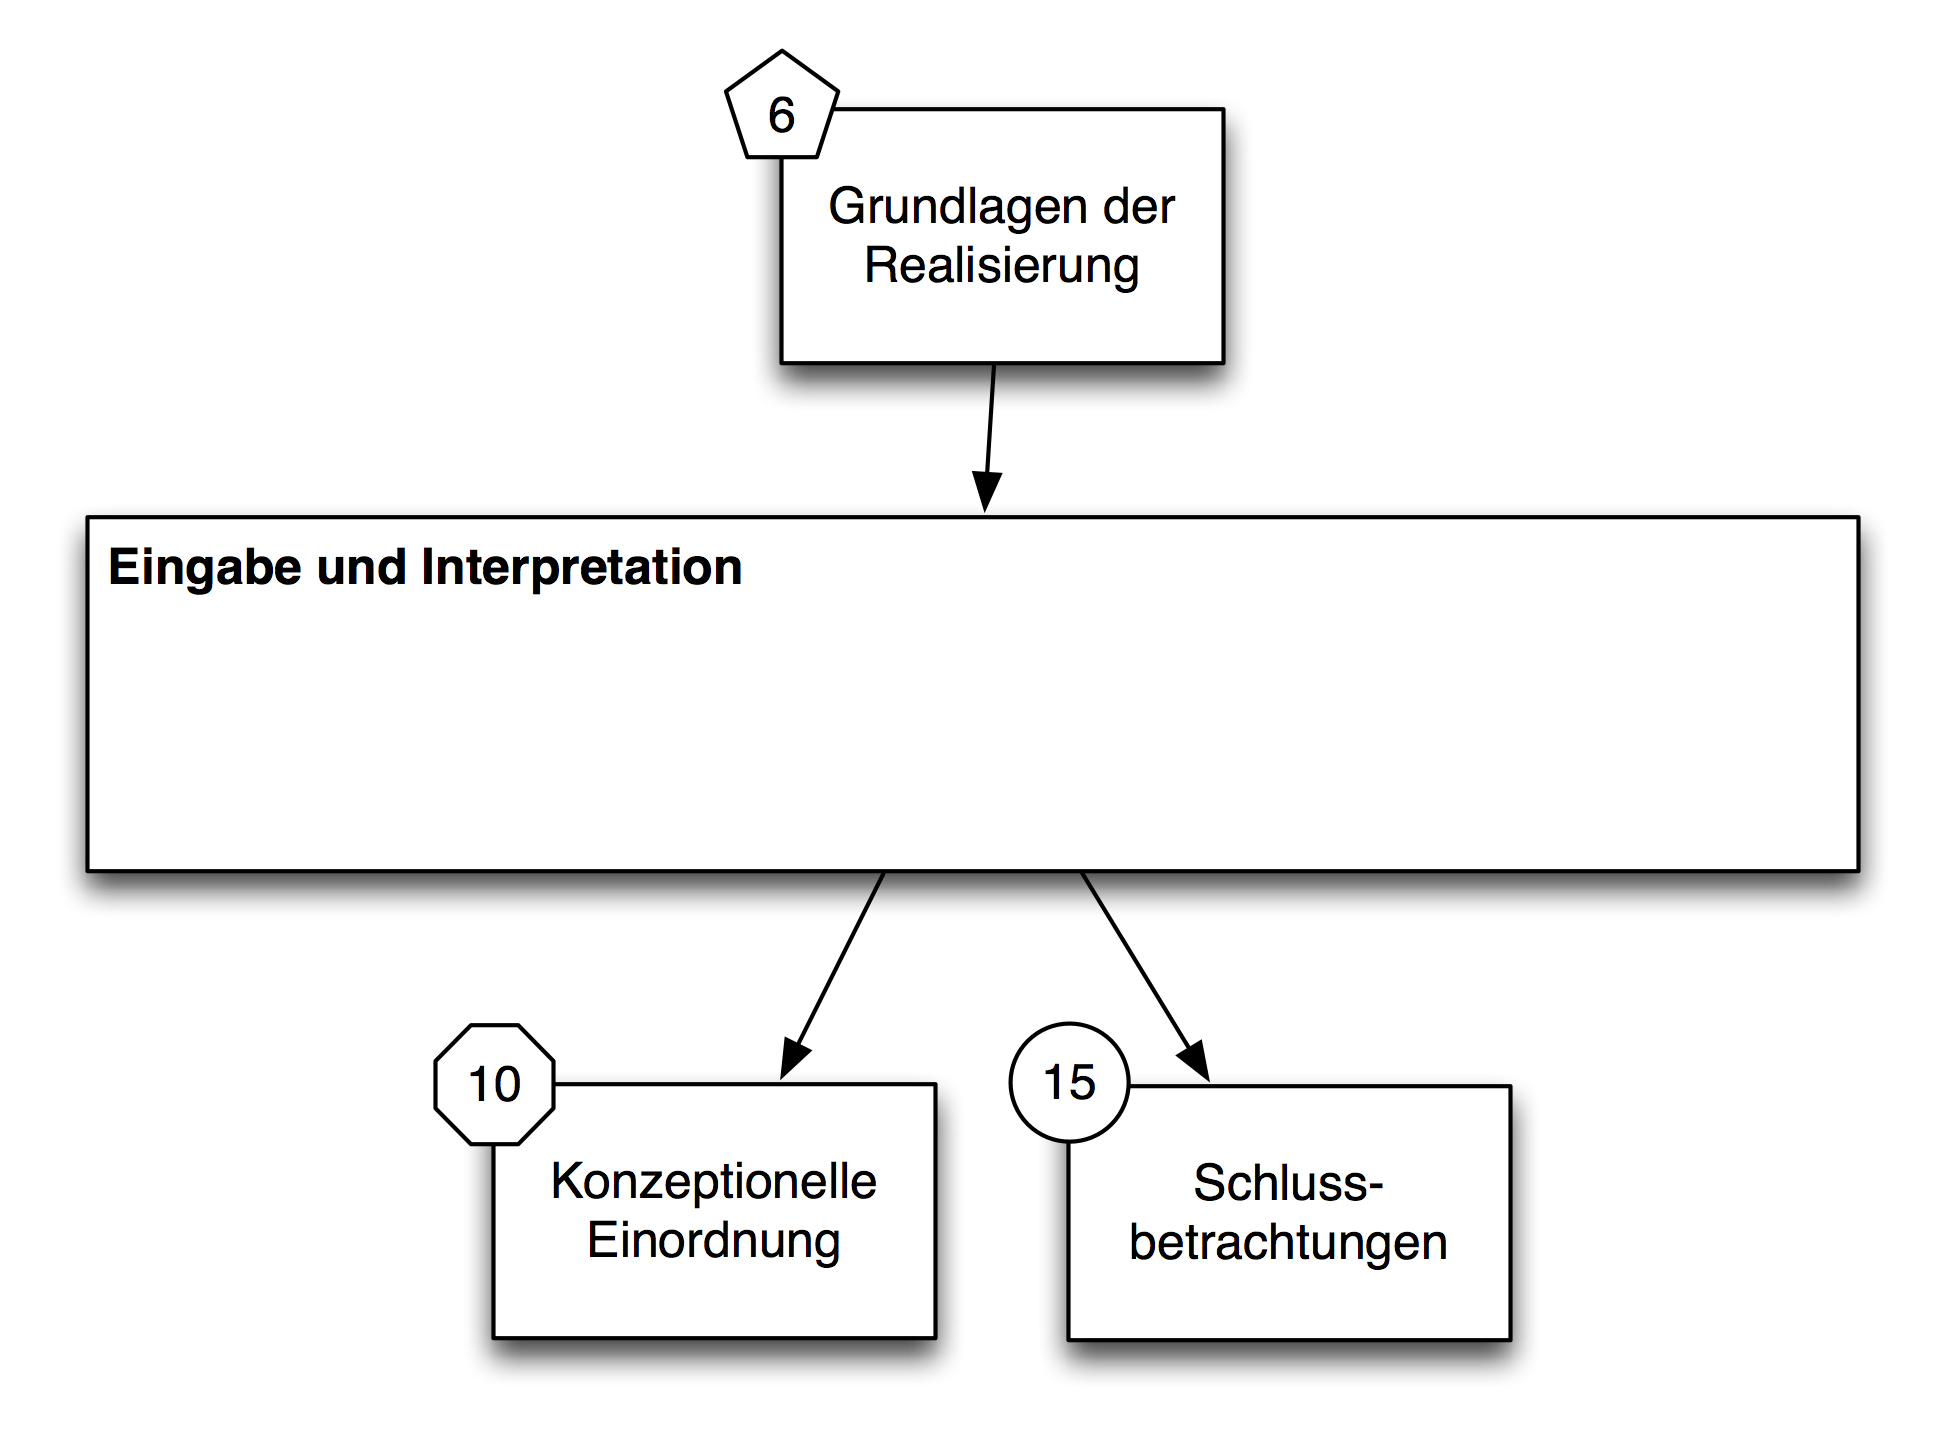
\includegraphics[scale=0.75]{img/Kontextgrafiken/k7.png}
	\caption{Kapitel „Eingabe und Interpretation“ im Gesamtzusammenhang}
	\label{fig:img_Kontextgrafiken_k7}
\end{figure}

Basierend auf dieser Entscheidung wird in den darauf folgenden beiden Abschnitten auf das Design der Hard- und Softwarekomponenten eingegangen, die unmittelbar der Eingabe von Information durch Benutzer dienen. Der Ausgabeaspekt wird hier bewusst ausgeklammert und im nächsten Kapitel beschrieben. Dieses Kapitel endet mit eine Beschreibung der Interpretationsroutinen, die aus den durch das Framework gelieferten Rohdaten höherwertige, anwendungsspezifische Information extrahieren und diese den nachgeordneten Software-Modulen zur Verfügung stellen.

\section{Möglichkeiten zur Erfassung von Benutzerinteraktion} % (fold)
\label{sec:möglichkeiten_zur_erfassung_von_benutzerinteraktion}

Im Gegensatz zu Systemen mit dezidierten Eingabegeräten (wie Tastatur oder Maus) ist die Informationseingabe bei Tangible Interfaces unmittelbar an physische Tokens gebunden, die unabhängig voneinander und gegebenenfalls auch simultan manipuliert werden können. Diese Manipulation muss von einer vorhandenen Infrastruktur erfasst und interpretiert werden. Der wesentliche Unterschied zu dezidierten Eingabegeräten besteht darin, dass die Manipulation des physischen Artefakts selbst für den Benutzer bedeutungstragend ist und nicht nur dem Zweck einer Zustandsänderung im digitalen Informationsraum dient. Dies impliziert, dass der Zustand der verwendeten Tokens bzw. der aktuelle Wert der relevanten Parameter (z.B. Position, Rotation, Form, ...) erfasst werden können, ohne die Bedeutung der Tokens noch deren Manipulierbarkeit in der realen Welt zu beeinträchtigen. Je nach Anwendungsfall kommen dafür mehrere unterschiedliche technologische Ansätze in Frage. Die Beurteilungskriterien die dabei zu berücksichtigen sind, umfassen die zu erhebenden Parametern und die notwendige Erfassungsrate des Zustandes der Tokens sowie die Anzahl der simultan zu erfassenden Tokens bzw. Parameter.

Im konkreten System muss -- wie in Kapitel XY beschrieben -- die planare Position von mehreren Tokens in Echtzeit (d.h. mehrmals pro Sekunde mit für den Benutzer nicht wahrnehmbaren Verzögerungen) erfasst werden. Neben der Position ist noch die Rotation eines Tokens als Raumparameter von Interesse. Bezüglich des Zustands eines Tokens muss erfasst werden können, ob es geöffnet oder geschlossen ist und ob es eingebettete Objekte enthält oder nicht. Mit diesen Anforderungen wird in den folgenden Unterabschnitten ein technologischer Ansatz zur Umsetzung der Interaktionserkennung ausgewählt.

\subsection{In Frage kommende technologische Ansätze} % (fold)
\label{sub:potentielle_technologische_ansätze}
Bei der Auswahl möglicher technologischer Ansätze zur Erfassung der Benutzerinteraktion müssen die zu erfassenden Parameter unterschiedlich behandelt werden. Konkret werden hier Ansätze zur Erfassung der Raumparameter (Position, Rotation) und Ansätze die Zustandsänderungen des Tokens erfassbar machen unterschieden. 

\subsubsection{Raumparameter} % (fold)
\label{ssub:raumparameter}
\index{Positionsbestimmung} 
Zur Erfassung von Raumparametern von Tokens bieten sich mehrere technologische Ansätze an. In Frage kommen für das konkrete Tabletop Interface nur Technologien, die eine Erfassung dieser Parameter mit einer Genauigkeit im Zentimeter- bis Millimeter-Bereich ermöglichen, da eine niedrigere Raumauflösung zu zu großen Ungenauigkeiten in der Positionsbestimmung führen würden, die einen Einsatz für das hier vorgestellte Werkzeug nicht erlauben würden. Im Folgenden werden die in Frage kommenden Technologien in ihren Grundzügen beschrieben und hinsichtlich ihrer Eignung für das konkrete System bewertet.

\paragraph{Optisch} % (fold)
\label{par:optisch}
\index{Positionsbestimmung!optisch} 
\index{Barcode} 

Optische Positionsbestimmung erfolgt mit Hilfe von Kamera-Systemen und Methoden der digitalen Bildverarbeitung. Die Kamera erfasst dabei die zu identifizierenden Tokens. Das resultierende Bild wird mit in Software umgesetzten Algorithmen ausgewertet. Dadurch können zumindest Identität und Position, zumeist aber auch weitere Raumparameter (wie Rotation) aller im Erfassungsbereich der Kamera befindlichen Tokens ermittelt werden. Neben dem optischen Erfassungsbereich bestimmen zudem die Auflösung der Kamera sowie die Größe der Tokens die letztendlich erfassbare Fläche. Optische Systeme sind bei schlechten oder wechselnden Lichtverhältnissen generell eher fehleranfällig und nicht robust gegen Verdeckungen von Tokens (etwa durch Gliedmaßen oder andere Tokens).

Hinsichtlich des Identifikationsansatzes können zwei Arten von Systemen unterschieden werden. \emph{Codebasierte} Systeme verwenden zur Identifikation eines Tokens einen von der Kamera erfassbaren Code (etwa einen „Barcode“), der eindeutig einem Token zugeordnet werden kann. \emph{Featurebasierte} Systeme identifizieren ein Token aufgrund seiner äußeren Eigenschaften, zumeist über dessen Form (Schattenriss). Letztere bieten den Vorteil, dass ein Token nicht durch das Anbringen eines zusätzlichen Codes optisch verändert werden muss. Der größte Nachteil besteht in der Eigenschaft, dass nur Token mit unterschiedlichen Formen eindeutig identifiziert werden können. Die eindeutige Identifikation von mehreren Tokens einer Bauart ist bei featurebasierten Systemen nicht möglich. Codebasierte Systeme verwenden zumeist nicht herkömmliche \gls{EAN}-Barcodes sondern robustere Systeme, bei denen eine Erkennung auch unter widrigen Beleuchtungsbedingungen oder niedrigen Bildauflösungen möglich ist und die zum Teil auch die Extraktion zusätzliche Information über weitere Raumparameter (wie Rotation, teilweise auch Parameter der dritten Dimension wie Neigung oder Entfernung) ermöglichen. 

Codebasierte Systeme können hinsichtlich der Art der Codierung der Identitätsinformation wiederum in zwei Klassen unterschieden werden. Eine Gruppe von Ansätzen integriert die eigentliche Nutzinformation, also im Wesentlichen die tokenspezifische Identifikationsnummer, direkt in den Code und ermöglicht so ein direktes Auslesen der Information (z.B. bei QRCode \citep{QR2008}). Die zweite Gruppe verwendet eine indirekte Zuordnung zwischen Token-ID und Code. Bei derartigen Ansätzen muss die Identität eines Tokens in einem Zwischenschritt über eine Mapping-Tabelle abgebildet werden, im Gegenzug ist die Ausgestaltung des Codes flexibler, im Allgemeinen kann dabei eine höhere Robustheit bei der Erkennung erreicht werden (z.B. ARToolkit \citep{Kato00}).

% paragraph optisch (end)

\paragraph{Kapazitiv} % (fold)
\label{par:kapazitiv}
\index{Positionsbestimmung!kapazitiv}  

Kapazitive Ansätze basieren auf der Änderung der Kapazität von Leiterbahnen, die durch deren Berührung mit leitfähigem Material verursacht wird. Ursprünglich wurde die Technologie zur Umsetzung von berührungssensitiven Oberflächen entwickelt, kann jedoch auch zum Tracking von Tokens verwendet werden. Im Gegensatz zu druckempfindlichen Oberflächen (klassischen „Touchscreens“) ist keine Druckausübung zur Erkennung notwendig, es können außerdem auch mehrere Tokens (bzw. Finger) gleichzeitig erkannt werden.

Technologisch bedingt müssen bei kapazitiven Ansätzen alle zu identifizierenden Objekte die Oberfläche des Systems berühren. In dieser Oberfläche ist ein Metallgitter eingebettet, zwischen dessen Adern eine elektrische Kapazität gemessen werden kann. Diese Kapazität verändert sich, sobald die Adern berührt werden (wobei die Token in einen entsprechend geeigneten Material ausgeführt sein müssen). Durch die lokale Änderung der Kapazität kann die Position einer Berührung festgestellt werden. Die Genauigkeit ist dabei durch die Rasterweite des Metallgitters beschränkt. Der größte Nachteil eines kapazitiven Ansatzes ist in diesem Kontext aber, dass die Identität eine Tokens nicht direkt festgestellt werden kann (die Kapazitätsänderung ist für alle Token identisch). Zudem ist die Extraktion weiterer Raumparameter (wie Rotation) nicht bzw. nur mit zusätzlichen Aufwand möglich. Die Vorteile von kapazitiven Systemen liegen in der hohen Robustheit der Erkennung auch bei widrigen Umgebungseinflüssen (Lichtverhältnisse, Schmutz) sowie der prinzipiell beliebig großen und beliebig geformten Oberfläche, die zur Erkennung verwendet werden kann.

Kapazitive Systeme eignen sich also zur Positionsbestimmung, nicht aber zur Identifikation von Tokens. Dies macht sie für den konkreten Anwendungsfall nur in Kombination mit einer anderen Technologie geeignet. 

% paragraph kapazitiv (end)

\paragraph{Elektromagnetisch} % (fold)
\label{par:elektromagnetisch}
\index{Positionsbestimmung!elektromagnetisch} 
\index{RFID}
 
Die Ausstattung von Tokens mit elektromagnetisch erfassbaren Einheiten (z.B. \gls{RFID}-Chips) ermöglicht ebenfalls die Erfassung von Raumparametern. Vorrangig eignet sich diese Technologie jedoch zur Identifikation von Tokens, die Positionsbestimmung kann nur mit erheblichem technischen Aufwand durchgeführt werden.

RFID-Chips (als Beispiel für einen elektromagnetischen Ansatz) sind passive Bauteile, die bei Energieversorgung durch ein elektrisches Feld aktiv werden und ihrerseits eine eindeutige Identifikationsnummer senden (im einfachsten Fall, komplexere Varianten sind möglich, werden hier aber nicht betrachtet). Historisch stammt die Technologie aus der Logistik und Warenwirtschaft und dient der Identifikation von Gütern und nicht der exakten Positionsbestimmung. Diese ist somit auch nur mittels erweiterter Infrastruktur möglich. Zum Auslesen eines \gls{RFID}-Chips wird ein Lesegerät mit Antenne benötigt. Aus der Feldstärke, mit der diese Antenne die Antwort des Chips empfängt, kann auf die Entfernung des Chips von der Antenne geschlossen werden. Durch Kreuzpeilung mit mindestens zwei Antennen, deren Position bekannt ist, kann somit auf die ungefähre Position des Chips (und damit des Tokens, in das dieser eingebaut ist) geschlossen werden. Durch den Einsatz von „Antennenarrays“ (matrixförmig angeordneten Antennen) mit geringer Reichweite ist so eine verhältnismäßig exakte (Größenordnung einige cm) Positionsbestimmung möglich. Die Feststellung der Ausrichtung eines Tokens (Rotation) ist auf diesem Wege allerdings nicht möglich. Die Identifikation eines Tokens ist jedoch unabhängig von Sichtkontakt und unmittelbarer Berührung und somit äußerst robust gegen Umgebungseinflüsse.

Elektromagnetische Systeme eignen sich wegen des hohen technischen Aufwandes bei gleichzeitig beschränkter Genauigkeit nur bedingt zur Feststellung von Raumparametern. Durch die Ausrichtung auf Extraktion der Identitätsinformation ist der Ansatz jedoch gut zur Kombination mit anderen Technologien wie kapazitiven Ansätzen geeignet, die ihre Stärken in der Bestimmung der Raumparameter haben.
 
% paragraph elektromagnetisch (end)

\paragraph{Akustisch} % (fold)
\label{par:akustisch}
\index{Positionsbestimmung!akustisch} 
\index{Ultraschall} 

Akustische Ansätze zur Positionsbestimmung basieren im Allgemeinen auf der Laufzeitmessung von Ultraschallwellen im Raum. Mit entsprechender Infrastruktur ist damit in einem begrenzten Bereich ein hochexakte Feststellung der Raumparameter in drei Dimensionen (Genauigkeit im mm-Berich) sowie die Identifikation von Tokens möglich.

Ultraschallbasierte Techniken zur Positionsbestimmung basieren auf dem Einsatz von Bakensendern an bekannten Positionen. Diese Sender werden zumeist an der Zimmerdecke montiert und senden periodisch einen Ultraschallimpuls aus. Dieser Impuls wird von den Tokens (die in diesem Fall aktive Bauteile mit Stromversorgung sind) empfangen, die daraufhin einen sie identifizierenden Impuls zurücksenden. Aus der Laufzeit zwischen Absetzen des Sendeimpuls und Empfangen des Antwortimpulses bei verschiedenen Baken lässt sich so die Position des Tokens im Raum feststellen. Problematisch ist hierbei jedoch die durch den auf sequentieller Zeitmessung basierenden Ansatz beschränkte Anzahl von verfolgbaren Tokens, wenn Echtzeit-Ansprüche gestellt werden. Zudem ist der Ansatz nicht robust gegen (akustisch) verdeckte Tokens. Eine Anfälligkeit gegenüber anderen Störeinflüssen besteht nicht. 

Für die Feststellung von Raumparametern sind ultraschall-basierte Systeme generell ausgezeichnet geeignet. Auch die Identifikation von Tokens ist prinzipiell möglich. Bei der Bewertung hinsichtlich des Einsatzes für Tabletop Interfaces ist jedoch zu bedenken, dass eine drei-dimensionale Positionierung nicht zu den allgemeinen Anforderungen zählt und nur in speziellen Anwendungsfällen sinnvoll sein kann. Zudem kann die Notwendigkeit von stromversorgten Tokens einen Nachteil bzw. ein Hindernis beim Einsatz darstellen.

% paragraph akustisch (end)

\paragraph{Bewertung} % (fold)
\label{par:bewertung}

Im konkreten Anwendungsfall ist die Feststellung der Identität sowie der planaren Position und Rotation von mehreren Tokens in hoher Genauigkeit sowie in Echtzeit gefordert. Aus oben genannten Gründen sind kapazitive und elektromagnetische Systeme im Einzeleinsatz nur bedingt geeignet. Akustische Systeme erscheinen für den Anwendungsfall als zu aufwändig und unflexibel und stoßen außerdem bei der Anzahl der simultan zu verfolgenden Tokens an ihre Grenzen.

Die Kombination von kapazitiven und elektromagnetischen Systemen ist grundsätzlich eine Möglichkeit, die in Betracht gezogen werden könnte. Auch optische Systeme genügen den Anforderungen und kommen damit in Frage. Der kombinierte Ansatz ist im Vergleich mit optischen Systemen als robuster gegen Störeinflüsse aus der Umgebung zu betrachten. Für optische Systeme sprechen hingegen die weitaus geringeren Aufwände für Infrastruktur und Tokens sowohl bei Anschaffung als auch bei Wartung und Betrieb. Durch die geringere Komplexität des Systems sind auch weniger potentielle Fehlerquellen vorhanden, was bei der Erstellung des Werkzeug-Prototypen hilfreich ist. Aufgrund dieser Aspekte und einer vergleichbaren zur erwartenden Erkennungsleistung wurde für die hier vorgestellten Anwendungfalls die Entscheidung getroffen, ein optisches System zur Bestimmung der Positionsparameter sowie der Identität der Tokens einzusetzen.

% paragraph bewertung (end)

% subsubsection raumparameter (end)

\subsubsection{Tokenzustand} % (fold)
\label{ssub:tokenzustand}

Hinsichtlich des Tokenzustands sind im Kontext des hier vorgestellten Anwendungsfalls Informationen zu erheben, die den Inhalt des Tokens betreffen. Wie in Kapitel XY beschrieben sind die Modellierungs-Tokens als Container ausgeführt, die geöffnet und geschlossen werden können und in die kleinere Tokens als Trägen von Zusatzinformation hineingelegt werden können. Die Auswahl eines Ansatzes, der die Identifikation des Öffnungs-Zustandes eines Tokens sowie dessen Inhalt erlaubt, ist Gegenstand dieses Abschnitts. Dazu wird grundlegend zwischen dem Einsatz von passiven Tokens und aktiven Tokens unterschieden. Passive Tokens besitzen keine zusätzliche Elektronik, die geforderten Informationen können lediglich durch die bereits vorhandene (optische) Infrastruktur festgestellt werden. Aktive Tokens werden hingegen mit zusätzlicher Elektronik zur Zustandsbestimmung ausgestattet, was allerdings eine Energieversorgung jedes Tokens bedingt.

\paragraph{Passive Token} % (fold)
\label{par:passive_token}
\index{Token!passive}
 
Bei passiven Tokens muss sichergestellt werden, dass die bereits vorhandene Infrastruktur die Zustandsänderungen eines Tokens erfassen kann. Das die vorhandene Infrastruktur auf optischen Technologien basiert, müssen sich alle Zustandsänderungen im äußeren -- durch die Kamera erfassbaren -- Erscheinungsbild eines Tokens wieder spiegeln.

Der Öffnungszustand eines Tokens kann durch Kameras einfach erfasst werden, wenn sich -- je nach eigesetzter Technologie -- durch das Öffnen der Umriss des Tokens verändert oder ein weiterer Code sichtbar wird bzw. der bestehende Code modifiziert wird. Diese Anforderung kann also durch passive Tokens erfüllt werden.

Zur Erfassung des Inhalts eines Container-Tokens sind zwei Ansätze denkbar. Einerseits kann der Inhalt eines Tokens zu einem bestimmten Zeitpunkt erfasst werden, andererseits ist auch eine Erfassung der Änderung des Tokeninhalts möglich (Erfassung des Vorgangs von Hineinlegen und Herausnehmen). Diese beiden Möglichkeiten sind hinsichtlich der Umsetzbarkeit mit passiven Token unterschiedlich zu beurteilen. Eine Erfassung das aktuellen Tokeninhalts ist mit optischen Systemen nur schwer möglich. Die einzige sich bietende Möglichkeit ist die Verwendung von transparenten Teilbereichen der Außenfläche eines Tokens. Damit ist es grundsätzlich möglich, den Inhalt eines Tokens mit einer externen Kamera zu erfassen. Sowohl bei feature- als auch code-basierten Ansätzen sind jedoch Verdeckungen, Verzerrungen oder zu geringe Kameraauflösung potentiell problematisch und lassen diesen Ansatz für den praktischen Einsatz als ungeeignet erscheinen.

Die Erfassung der Änderung des Tokeninhalts lässt sich mit optischen Systemen einfach implementieren. So kann der Vorgang des Hineinlegens als auch des Herausnehmens von einer Kamera erfasst werden. Die größte Herausforderung hierbei ist die Identifikation des Tokens, das eingebettet wird. Hier kann es wiederum durch Verdeckungen zu Erkennungsschwierigkeiten führen, was in diesem Fall einen permanent fehlerhaften Modellzustand zur Folge hat, der sich im Falle wiederholter Fehlerkennungen sogar inkrementell zu größeren Abweichungen führen kann kann. Diesem Umstand kann lediglich durch eine explizite Aktion des Benutzers Rechnung getragen werden, der das betreffende einzubettende Token ins Sichtfeld der Kamera halten muss, bis das System Feedback über eine erfolgreiche Erkennung gibt. Diese Lösung erscheint allerdings hinsichtlich der Anforderung, die Technologie für den Benutzer vollkommen in den Hintergrund treten zu lassen, als eher suboptimal.

% paragraph passive_token (end)

\paragraph{Aktive Token} % (fold)
\label{par:aktive_token}
\index{Token!aktive}

Aktive Tokens beinhalten zusätzliche Sensorik, die die Erfassung des Tokenzustands ermöglicht. Derartige Tokens benötigen allerdings eine Energieversorgung und müssen über eine Möglichkeit zur Datenübertragung verfügen, um den Tokenzustand an das System zu übermitteln. Weiters ist im Allgemeinen eine Steuereinheit notwendig, um die Sensoren zu kontrollieren, die Daten zu aggregieren und letztendlich zu übertragen.

Im konkreten Fall einer optisch arbeitenden Infrastruktur bietet sich eine (ggf. aufladbare) Batterie als Energiequelle an, um im Kamerabild Verdeckungen durch ansonsten eventuell zu verwendende Kabel zu vermeiden. Eine Stromversorung über die Oberfläche (wie z.B. im Pin \& Play System \citep{Van-Laerhoven03} vorgestellt) scheidet hier aus, da die Blöcke dann mit Krafteinsatz auf die Oberfläche gesetzt werden müssten und nicht verschoben werden können. 

\index{SmartIT} 
Als Steuerungseinheit bietet sich neben selbst auf der Basis von Mikrocontrollern wie dem PIC oder 8051 \citep{James97} konzipierten Systemen auch Plattformen an, die explizit für den Anwendungszweck der Ansteuerung von Sensoren oder Aktuatoren und der Kommunikation mit einem Basissystem gefertigt werden. Exemplarisch kann hier die Smart-ITs-Plattform \citep{Gellersen04} angeführt werden, die neben der flexiblen Ansteuerbarkeiten von unterschiedlichen Sensoren bereits Module zur Vernetzung untereinander und mit zentralen Diensten in der Infrastruktur anbietet.

\index{ZigBee} 
\index{Bluetooth} 
Aus den eben angeführten Gründen erscheint zur Datenübertragung eine drahtlos arbeitende Technologie am geeignetsten. Aufgrund der geringen benötigten Reichweite und der Anforderung, möglichst energieeffizient zu arbeiten, bieten sich die Technologien „Bluetooth“ \citep{Bluetooth-SIG07} und „ZigBee“ \citep{ZigBee07} an. Bluetooth erreicht höhere Übertragungsraten, ist aber in der Anzahl der gleichzeitig verwendbaren Geräte (max. 7) für den hier vorgestellten Anwendungsfall zu beschränkt. Ein ZigBee-Netz kann mit bis zu 255 Geräten gleichzeitig arbeiten und ist außerdem im Einsatz energiesparender. Für den gegebenen Anwendungsfall erschiene also ZigBee als geeignete Technologie (und wurde auch bereits in \citep{Ferscha08} in einem ähnlichen Anwendungsfall erfolgreich eingesetzt).

Zur Feststellung des Öffnungsstatus eines Container-Tokens bieten sich bei aktiven Sensortechnologien mehrere Möglichkeiten an. Der Einsatz eines Schaltelements, das beim Öffnen den Kontakt herstellt oder unterbricht, erscheint als eine nahe liegende Lösung. Auch der Einsatz eines Drehelements am Angelpunkt des Öffnungsschaniers, dessen elektrische Eigenschaften (z.B. Widerstand oder Kapazität) mit dem Öffnungswinkel ändern, kann angedacht werden. Damit ist nicht nur eine Unterscheidung zwischen den Zuständen „offen“ oder „geschlossen“ sondern auch die Identifikation von Zwischenzuständen möglich.

Der Inhalt eines Container-Tokens kann ebenfalls mit unterschiedlichen Technologien erfasst werden. Die Zielsetzung ist hier nicht der Positionsbestimmung der eingebetteten Tokens sondern lediglich die Feststellung der Identität. Naheliegend ist hierzu der Einsatz von elektromagnetischen Ansätzen wie oben beschrieben. Durch das Anbringen von z.B. \gls{RFID}-Chips an den einzubettenden Tokens sowie eines Lesegeräts im Container-Token kann die Identifikation robust durchgeführt werden. Alternativ bieten sich Systeme an, die auf Gewichtsmessung basieren. Über einen in das Containertoken eingebauten Sensor wird dabei das Gesamtgewicht der eingebetteten Tokens bestimmt. Bei entsprechender Konzeption der einzubettenden Tokens (unterschiedliche Gewichte) kann aus dem Gesamtgewicht auf die tatsächlich enthaltenen Tokens geschlossen werden. Ein Nachteil dieses Ansatzes ist die beschränkte Anzahl von erfassbaren Tokens und die notwendige exakte Fertigung jedes einzelnen Tokens, da es bei Gewichtsabweichungen zu Fehlerkennungen kommt.

% paragraph aktive_token (end)

\paragraph{Bewertung} % (fold)
\label{par:zustand_bewertung}

Hinsichtlich der erreichbaren Flexibilität und zu erwartenden Servicequalität wäre in diesem Abschnitt eine Entscheidung zugunsten aktiver Tokens zu treffen. Im Gesamtkontext betrachtet und unter Berücksichtigung der Entscheidung für optische Systeme zur Bestimmung der Positionsparameter ist diese Wahl jedoch zu relativieren. Wie oben beschrieben, erlaubt eine auf optischen Systemen beruhende Infrastruktur grundlegend die Umsetzung der geforderten Funktionalität. Gleichzeitig wird die Komplexität des Systems massiv reduziert und die Erstellung zusätzlicher Tokens vereinfacht (da keine zusätzliche Elektronik notwendig ist). Der Wegfall von Energieversorgung und Sensorlogik in den Token reduziert deren Gewicht und ermöglicht gleichzeitig mehr Platz für einzubettende Tokens.

Für den hier beschriebenen Anwendungsfalls bzw. die prototypische Umsetzung des Werkzeugs wird deshalb auf aktive Tokens verzichtet und der Einsatz von passiven Tokens bevorzugt. Der Mehraufwand in Erstellung und Wartung des Systems beim Einsatz aktiver Tokens wiegt in der Gesamtheit betrachtet die zu erwartende höhere Erkennungsqualität nicht auf.
% paragraph zustand_bewertung (end)
% subsubsection tokenzustand (end)

% subsection potentielle_technologische_ansätze (end)
\subsection{In Frage kommende Frameworks} % (fold)
\label{sub:verfügbare_frameworks}

Unter Anbetracht der im vorherigen Abschnitt getroffenen grundlegender Technologieentscheidung zugunsten optischer Erkennungstechnologie mit passiven Tokens werden nun unterschiedliche Frameworks betrachtet, die die Umsetzung dieses Ansatzes erlauben. Dabei sind zwei Klassen von Frameworks zu unterscheiden: 

\emph{Generische Frameworks für Tangible Interfaces} ermöglichen generell die Koordination von Services, die die Kopplung von Sensoren und Aktuatoren mit Interpretations-Logik und letztendlich konkreten Applikationen erlauben. Sie gehen dabei nicht auf konkrete Sensortechnologien (wie die hier verwendeten optischen Ansätze) ein sondern versuchen eine Abstraktionsebene einzuführen, die die Applikationen von der konkreten Technologie entkoppelt und damit flexibler macht. 

\emph{Frameworks für video-basierten Input für Tangible Interfaces} sind spezialisierte Produkte, die konkret für die Umsetzung von optischen Ansätzen zur Eingabe von Daten bei Tangible Interfaces ausgelegt sind. Durch die Spezialisierung auf optische Identifikation liegt ihr Vorteil im geringeren technischen Aufwand bei der Einrichtung und auch während des Betriebs. Echtzeit-Anforderungen sind oft nur mit spezialisierten Frameworks zu erfüllen. Eine Kombinationsmöglichkeit zwischen Produkten der beiden Kategorien ergibt sich beim Einsatz eines spezialisierten Frameworks als Eingabe-Modul für eine generisches Framework. Durch diesen Ansatz kann die einfache Inbetriebnahme spezialisierter Frameworks mit der Flexibilität generischer Frameworks zusammengeführt werden. 

\subsubsection{Generische Frameworks} % (fold)
\label{ssub:generische_frameworks}

Generische Frameworks zur Behandlung von Input und Output bei Tangible Interfaces sind historisch nicht exakt von anderen Frameworks abzugrenzen, die im Umfeld des Ubiquitous bzw. Pervasive Computing \citep{Weiser91} entwickelt wurden. Von konkreter Technologie abstrahierende Frameworks wurden erstmals im Zusammenhang mit „Context-aware Computing“ \citep{Schilit94} erwähnt, um Applikationen die Möglichkeit zu bieten, Information aus der Umgebung über beliebige Sensoren zu erfassen, diese zu aggregieren und zu interpretieren. Aufbauend auf dieser Interpretation sollen Aussagen über den aktuellen Zustand der Umgebung (den „Kontext“) getroffen werden können, die die Applikationen wiederum zur Adaption benutzen können. Der Rückkanal, also die Ansteuerung von Aktuatoren, wurde erst in späteren Entwicklungen berücksichtigt. Ein Großteil der Systeme dient explizit nicht der Erstellung von marktreifen Applikationen sonderen widmet sich eher der Umsetzung von „Rapid Prototyping“-Ansätzen im Bereich der Tangible Interfaces. Begründet wird dies mit der oft suboptimalen Ressourcen-Ausnutzung, die mit der Generalisierung und Flexiblisierung des Frameworks einhergeht. 

Die Aufzählung der hier beschriebenen Frameworks erhebt keinen Anspruch auf Vollständigkeit. Bei der Auswahl wurde darauf geachtet, historische bzw. für den konkreten Anwendungsfall geeignete Ansätze aufzunehmen und in ihren wesentlichen Eigenschaften zu beschreiben.

\paragraph{Context Toolkit} % (fold)
\label{par:context_toolkit}
\index{Context Toolkit}
 
Das Context Toolkit \citep{Dey01} ist das historisch erste Framework, das versucht, die starre Verbindung zwischen Sensoren und Applikationslogik aufzubrechen. Es führt eine konfigurierbare Schicht ein, die eine schnellere, generischere Applikationsentwicklung ermöglicht und die Wiederverwendung einmal entwickelter Komponenten ermöglicht.

Konzeptuell existieren im Framework drei Arten von Komponenten: „Context Widgets“, „Context Interpreters“ und „Context Aggregators“. „Context Widgets“ implementieren die Ansteuerung beliebiger Software- und Hardwaresensoren und sind für das Sammeln von Information über die Umgebung zuständig. Sie vermitteln zwischen der physischen Umgebung und den konzeptionell höher liegenden Komponenten indem sie die unverarbeiteten Kontextdaten mittels einer geeigneten Schnittstelle kapseln und bestimmte Funktionen zur ersten Auswertung der Rohdaten ausführen. Eine Anwendung kann diese Daten verwenden, ohne dass sie Detailkenntnisse über die zugrunde liegenden Sensortechnologien haben muss. „Context Interpreter“ aggregieren die Sensordaten zu komplexeren Kontextinformationen d.h. sie konvertieren und interpretieren die Daten mehrerer „Context Widgets“ und versuchen diese zu einheitlichen Clustern zusammenzufassen. „Context Aggregators“ dient der Zusammenführung verschiedener Kontextinformationen die für bestimmte Anwendungen relevant sind. „Context Aggregators“ bilden damit die Schnittstelle zu den eigentlichen Applikationen.

Das Context Toolkit bietet nicht nur eine Softwareschnittstelle zu physischen Sensoren, es trennt auch die Akquisition und Repräsentation von der Auslieferung der Daten an kontextsensitive Applikationen.
% paragraph context_toolkit (end)

\paragraph{SiLiCon Context Framework} % (fold)
\label{par:silicon_context_framework}

Das SiLiCon Context Framework \citep{Beer03} ist ein Vertreter jener Klasse von Frameworks, deren Verhalten zur Laufzeit dynamisch konfigurierbar ist. Dies bedeutet im konkreten Fall, dass Applikationen, die auf Basis des SiLiCon Context Framework erstellt wurden, ihr Verhalten und ihren Aufbau aufgrund eintretender Ereignisse verändern können. Dies betrifft sowohl das Aktivieren und Deaktivieren von Input- und Output-Kanälen also auch die Veränderung der Interpretation der eingehenden Information und die Reaktion darauf. Das Framework wurde entworfen, um Szenarien beschreiben zu können, in denen interaktive Systeme kontextsensitiv -- d.h. abhängig vom aktuellen Zustand ihrer Umwelt -- reagieren müssen.

Die grundlegenden Bausteine des SiLiCon Context Framework sind „Entitäten“, die Objekte der realen Welt konzeptionell abbilden. Diese „Entitäten“ besitzen „Attribute“, also Eigenschaften, mit Hilfe derer die Entität näher beschrieben wird. Über „Attribute“ kann die Wahrnehmung einer „Entität“ von deren Umwelt sowie deren Interaktionsmöglichkeiten mit derselben beschrieben werden. Mit Hilfe von \gls{ECA}-Regeln  wird beschrieben, auf welche Wahrnehmung der Umwelt („Event“) eine Entität unter welchen Bedingungen („Condition“, formuliert auf Basis des internen Zustands der Entität) mit welchen Aktivitäten („Acti“on) reagiert. Diese Regeln können zur Laufzeit dynamisch verändert und nachgeladen werden. Außerdem ist es möglich, in „Actions“ das Nachladen von Entitäten oder das Hinzufügen oder Entfernen einzelner Attribute durchzuführen \citep[][S. 90]{Oppl04}.

Das SiLiCon Context Framework abstrahiert durch seine konzeptionelle Struktur mit dem Einsatz von „Entitäten“ und „Attributen“ nicht so stark von der realen Welt wie das zuvor beschriebene Context Toolkit -- die Abbildung ist im ersten Schritt „direkter“ und muss erst im zweiten Schritt technisch konkretisiert werden, ein klassischer Softwareengineeringprozess (im Sinne von „Analyse -- Design -- Implementierung“) wird damit vollständiger (auch in den ersten Phasen) durch das Framework abgebildet und unterstützt. 

% paragraph silicon_context_framework (end)

\paragraph{Papiermaché} % (fold)
\label{par:papiermaché}
Papiermaché \citep{Klemmer04} ist eines der ersten Rapid Prototyping Frameworks, die dezidiert zur Entwicklung von Tangible Interfaces entworfen wurden. Es fokussiert auf die Anbindung von Inputtechnologien für passive Objekte (RFID oder optische Ansätze) und stellt Applikationen eine abstrahierte Sicht auf die reale Welt zur Verfügung (in Form einer Repräsentation der erfassten Objekte als „Phobs“ -- Physical Objects --, die die für die jeweilige Applikation relevanten Daten kapseln). Andere Eingabekanäle sind in der zur Verfügung stehenden Implementierung nicht vorgesehen -- die Einordnung als generisches Framework ist aufgrund der übrigen Architektur trotzdem gerechtfertigt. Der Benachrichtigungsmechanismus erfolgt wie im Context Toolkit ereignisgesteuert -- d.h. jede Änderung der erfassten Umgebung generiert ein Ereignis im Framework, das an die weiterverarbeitende Applikation weitergeleitet wird.

Im Sinne des Rapid Prototyping stellt Papiermaché als einziges hier betrachtetes Framework eine Art Entwicklungs- und Laufzeitumgebung für Tangible Interfaces zur Verfügung. Mittels dieser können Applikationsentwickler etwa Eingabekanäle auswählen und die Interpretation der Rohdaten zur Laufzeit konfigurieren. Die Entwicklungsumgebung macht die zugrundeliegende Hardware für den Entwickler dabei transparent, er muss sich also nicht um die Details der technischen Anbindung kümmern, ist dafür aber auf die bereits implementierten Hardware-Schnittstellen beschränkt. Die Interpretation der Daten beschreibt der Entwickler in Source Code, der über definierte Schnittstellen in das Framework eingebunden wird. Über ein Monitoring-Interface kann die Arbeit des Frameworks zur Laufzeit beobachtet werden, um so z.B. Fehlverhalten oder ineffiziente Konfigurationen aufzudecken.

Papiermaché versucht, mittels der Integration von vorgegebenen Eingabekanälen, die konfiguriert werden können, einen Teil der Komplexität bei der Entwicklung von Tangible Interface abzumildern. Der übrige konzeptionelle Aufbau ähnelt dem Context Toolkit -- Interpretation der Daten und Verwendung in einer Applikation sind konzeptionell getrennt. Papiermaché ist in seiner Ausrichtung auf den Einsatz für Tangible Interfaces ausgelegt, die auf der Manipulation von einzelnen physischen Objekten und der Beziehungen zwischen diesen beruht. Es ist damit nicht so flexibel einsetzbar wie die anderen betrachteten Frameworks, erscheint aber für den hier vorgestellten Anwendungsfall grundsätzlich geeignet.
% paragraph papiermaché (end)

\paragraph{TUIpist} % (fold)
\label{par:tuipist}

Das TUIpist-Framework \citep{Furtmuller07} wurde im Zusammenhang mit der hier vorgestellten Arbeit entwickelt \citep{Furtmuller07a}. TUIpist verfolgt einen ähnlich modularen Ansatz wie die anderen hier vorgestellten Frameworks, setzt jedoch zur Koordination der Module untereinander einen daten-zentrierten Ansatz -- auf dem LINDA-Konzept \citep{Carriero89} beruhende Tuplespaces -- ein. Die konzeptionelle Modulstruktur ist ähnlich der Aufteilung, die bereits von \citet{Dey01} im Context Toolkit vorgeschlagen wurde.

Die grundlegenden Module, die im Framework verwendet werden, sind „Sensoren“, „Aggragtoren“ und „Anwendungen / Aktuatoren“ (siehe Abbildung \ref{fig:img_ImplementierungInput_TUIpist}). „Sensor“-Module binden externe Datenquellen an das Framework an. Sie enthalten dazu eine sensor-spezifische Komponente, die die Schnittstelle zur jeweiligen Hard- bzw. Software bildet. Über diese Schnittstelle gelieferte Daten werden in einer zweiten Komponente vorverarbeitet und soweit abstrahiert, dass die Datenrepräsentation unabhängig von der die Daten liefernden Sensortechnologie ist (z.B. Abbildung von \gls{GPS}-Koordinaten auf logische Positionsinformation, die auch aus anderen Quellen stammen könnte). „Aggregatoren“ fassen die Information mehrerer „Sensor“-Module zusammen und interpretieren ggf. einander ergänzende oder auch widersprechende Information. Sie werden immer aktiv, wenn neue Sensordaten zur Verfügung stehen und aktualisieren dabei die Information über den Gesamtzustand der den Framework bekannten Umwelt. „Anwendungen / Aktuatoren“ bilden letztendlich die Schnittstelle zu konkreten Applikationen, die ihr Verhalten an den aktuellen Umweltzustand anpassen bzw. diesen darstellen oder Aktuatoren, die basierend auf dem aktuellen Umweltzustand Aktionen in dieser setzen. „Anwendungen / Aktuatoren“ filtern dabei wieder den von „Aggregatoren“ gelieferten Gesamtzustand der bekannten Umwelt und liefern nur die für die Applikation relevanten Daten aus. Dabei kann erneut eine Nachverarbeitung der Daten, z.B. im Sinne einer Anpassung an eine externe Schnittstelle, erfolgen.

\begin{figure}[htbp]
	\centering
		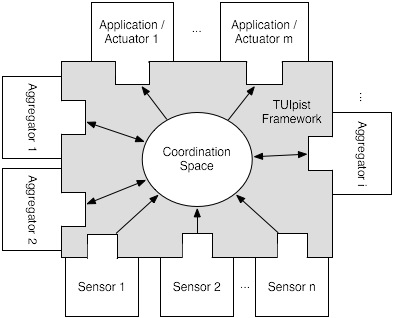
\includegraphics[height=2in]{img/ImplementierungInput/TUIpistArchitecture.jpg}
	\caption[Architektur des TUIpist-Framework]{Architektur des TUIpist-Framework \citep{Furtmuller07a}}
	\label{fig:img_ImplementierungInput_TUIpist}
\end{figure}

Die Verbindung der Komponenten erfolgt wie erwähnt datenzentriert. Eine wesentliche Eigenschaft dieses Ansatzes ist, dass keine explizite Verknüpfungen zwischen den Modulen definiert werden. Die Zuordnung erfolgt vielmehr indirekt durch die Daten selbst. Jedes Modul kann Datensätze („Tuple“) in einem definierten Format generieren und in einen gemeinsam genutzten Datenraum -- den „Tuplespace“ -- stellen. Andere Module können nun Anfragen an den „Tuplesp“ace stellen, ob Daten, deren Struktur oder Inhalt gewissen Kriterien entspricht, vorhanden sind. Ist dies der Fall, können diese Daten aus dem „Tuplespace“ entnommen werden und nach erfolgter Verarbeitung in modifizierter Form wieder eingestellt werden (siehe Abbildung \ref{fig:img_ImplementierungInput_TUIpistOperation}). Das „Tupel“space-Konzept erlaubt auch eine dynamische Erweiterung bzw. Veränderung sowohl der Ein- und Ausgabekanäle als auch der internen Datenverarbeitung zur Laufzeit, indem zusätzlich Module am „Tupelspace“ registriert werden. Durch die lose Koppelung der Module muss keine zusätzliche Konfiguration an anderen Modulen oder am „Tuplespace“ selbst vorgenommen werden.

\begin{figure}[htbp]
	\centering
		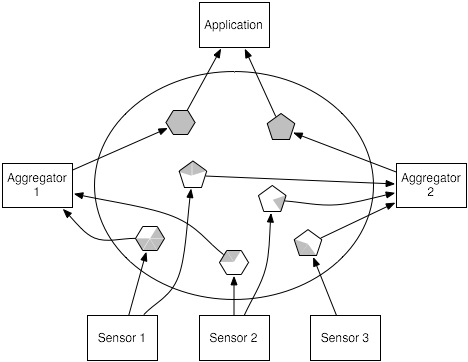
\includegraphics[height=2in]{img/ImplementierungInput/TUIpistOperation.jpg}
	\caption[Zusammenspiel der Komponenten in TUIpist]{Zusammenspiel der Komponenten in TUIpist \citep{Furtmuller07a}}
	\label{fig:img_ImplementierungInput_TUIpistOperation}
\end{figure}

Die Implementierung von TUIpist auf Basis des Java Jini-Frameworks \citep{Arnold99} ermöglicht eine Verteilung der einzelnen Module einer Applikation auf unterschiedliche Rechner (im Sinne eines „verteilten Systems“ \citep{Stary94}) ohne zusätzlich vom Implementierer zu berücksichtigenden Koordinationsaufwand. Es können damit auch (räumlich) entfernte Sensoren oder Webapplikationen angebunden werden und der ggf. auftretende Rechenaufwand zur Aggregation oder Interpretation von Daten auf mehrere Rechner verteilt werden.
% paragraph tuipist (end)

% subsubsection generische_frameworks (end)

\subsubsection{Frameworks für video-basierten Input} % (fold)
\label{ssub:frameworks_für_video_basierten_input}

Im Gegensatz zu den eben beschriebenen generischen Frameworks wurden die hier vorgestellten Frameworks explizit für die Behandlung von video-basiertem Input entwickelt. Wie oben bereits erwähnt, stehen die hier beschriebenen Frameworks mit den eben angeführten generischen Frameworks insofern in Zusammenhang, also dass sie zumeist als Sensor-Komponente in generischen Ansätzen eingesetzt werden können. In ihrer grundlegenden Ausrichtung sind sie jedoch zumeist für den unmittelbaren Einsatz in einer Endanwendung konzipiert.

Die hier vorgestellten Systeme implementieren den Ansatz des code-basierten optischen Trackings. Feature-basierte Ansätze kommen im konkreten Anwendungsfall nicht in Frage, da zur Modellierung eine Vielzahl von gleichartigen Objekten eingesetzt werden, die sich in ihrem äußeren Erscheinungsbild nicht unterscheiden und damit in feature-basierten Ansätzen nicht eindeutig identifiziert werden können.

Wie bereits im letzten Abschnitt erhebt auch die hier angeführte Aufzählung keinen Anspruch auf Vollständigkeit. Neben der Darstellung der historischen Entwicklung des Feldes und der Beschreibung von in Forschung und Praxis relevanten Ansätzen wurde bei der Auswahl vor allem auf freie Verwendbarkeit und Zugriff auf den Source-Code der Erkennungsroutinen geachtet, da die Notwendigkeit applikationsspezifischer Anpassungen nicht auszuschließen war (etwa um benötigte aber nicht direkt unterstützte Parameter zu extrahieren).

\paragraph{AR Toolkit}\label{par:artoolkit}
\index{AR Toolkit}
Das AR Toolkit („Augmented Reality Toolkit“) \citep{Kato00} ist historisch das erste in breitem Umfang eingesetzte Framework zur optischen Identifikation von Elementen in der realen Welt. Das AR Toolkit verwendet zur Identifikation Marker, in die selbst keine Information codiert ist, und eine Mapping-Tabelle zur Verknüpfung mit digitaler Information. Die Marker des AR Toolkit (siehe Abbildung \ref{fig:img_ImplementierungInput_artoolkit}) werden durch Mustererkennung identifiziert und weisen bis auf den schwarzen Rahmen, der einen Marker begrenzt, keine verpflichtenden Elemente auf. Die Form der Marker ist also vorgegeben, ihr Inhalt kann frei gestaltet werden, zur Identifikation ist es aber notwendig, das die zu erkennenden Marker im Vorhinein beim Framework registriert werden. 

\begin{figure}[htbp]
	\centering
		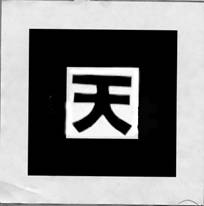
\includegraphics[height=1in]{img/ImplementierungInput/artoolkit.jpg}
	\caption[AR Toolkit Marker]{AR Toolkit Marker (Quelle: www.hitl.washington.edu/artoolkit/)}
	\label{fig:img_ImplementierungInput_artoolkit}
\end{figure}

Das AR Toolkit ist auf die Verwendung in Anwendungen im Bereich der Augmented Reality ausgelegt und liefert die aus dem Bild extrahierte Information in einer Form, die eine Weiterverarbeitung mittels Frameworks aus dieser Domäne möglich macht. Konkret werden Raumparameter als Transformationsmatrizen ausgegeben, die eine direkte Umsetzung der Information in eine Darstellung mittels OpenGL ermöglichen. Die Anbindung von Kameras an das Framework wird über plattformspezifische Treiber realisiert, das AR Toolkit selbst empfängt einen Bildstrom, den es auswertet. Die Erkennungssoftware ist in C implementiert, bietet aber Wrapper für andere Programmiersprachen (unter anderem Java). Sie wird als Bibliothek in die eigentliche Applikation eingebunden.

% paragraph artoolkit (end)

\paragraph{Visual Codes}\label{par:visualcodes}
\index{Visual Codes}

Das Visual Codes System \citep{Rohs05} ist ein Vertreter der direkt codierenden Ansätze, d.h. dass die Nutzinformation ohne Zwischenschritt direkt aus dem Code extrahiert werden kann. Im Gegensatz zu den standardisierten und kommerziell genutzten Code-Formate QR-Code \citep{QR2008} oder Datamatrix \citep{GS108}, die eine Kapazität von bis zu einigen hundert Byte haben, bietet das Visual Code System lediglich 83 Bits an Nutzinformation an (siehe Abbildung \ref{fig:img_ImplementierungInput_visualcodes}), was dazu führt, das in vielen Anwendungsfällen ein Mapping durch die Anwendung durchgeführt wird, um die zu verwaltende Information abbilden zu können.

\begin{figure}[htbp]
	\centering
		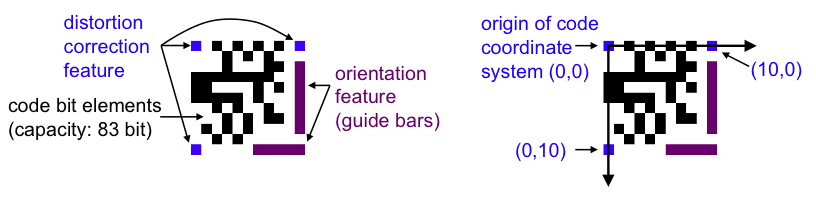
\includegraphics[height=3cm]{img/ImplementierungInput/visualcodes.png}
	\caption[Visual Codes -- Aufbau und Features]{Visual Codes -- Aufbau und Features (übernommen von \citet{Rohs04})}
	\label{fig:img_ImplementierungInput_visualcodes}
\end{figure}


Der Vorteil des Visual Code Systems liegt in der Auswertbarkeit einer Vielzahl von Raumparametern bei gleichzeitig geringem Bedarf an Rechenkapazität. In der Standardimplementierung werden neben der Position und der Rotation in der Ebene auch die Neigungsparameter im Raum extrahiert. Der Erkennungsalgorithmus läuft dabei in Echtzeit und kann unverändert sogar auf Java-fähigen Mobiltelefonen ausgeführt werden. Durch die relativ geringe Datendicht der Codes reichen dementsprechend auch verhältnismäßig niedrig auflösende Bilder (z.B. 320 x 240 Bildpunkte) für eine Erkennung aus. Wie alle anderen optischen Ansätzen leidet das Visual Code System unter Erkennungsproblemen bei wechselnden Lichtverhältnissen und insbesondere bei schlechtem Kontrast. Diese Verhalten kann in der vorliegenden Implementierung auch nicht durch Anpassung der Kameraparameter (Bildverstärkung o.ä.) korrigiert werden.

Das Visual Code System muss von auf ihm aufbauenden Applikationen direkt auf Source-Code-Ebene eingebunden werden, eine vorgegebene externe Schnittstelle existiert nicht. Anbindungsroutinen für Kameras existieren nur für Mobiltelefone und müssen für andere Plattformen ggf. neu erstellt werden.

% paragraph visualcodes (end)

\paragraph{ReacTIVision}\label{par:reactivision}
\index{ReacTIVision}
ReacTIVision \citep{Kaltenbrunner07} ist ein frei verfügbares Framework zu optischen Erkennung von Codes in Echtzeit. ReacTIVision arbeitet mit proprietären Codes (siehe Abbildung \ref{fig:img_ImplementierungInput_ReactivisionCode}), in denen die Information nicht an bestimmte Positionen sondern im Wesentlichen in die Anzahl und Schachtelung der Schwarz-Weiß-Übergänge codiert ist. Der Umfang der direkt in einen Marker codierbaren Information ist damit beschränkt und nicht direkt auf ein binäres Codierungsschema abbildbar. Deswegen wird ein Mapping-Ansatz verwendet, um die eigentliche Nutzinformation auf Codes abzubilden. Grundsätzlich wäre jedoch die direkte Codierung eine beschränkten Anzahl von Bits möglich, ist aber nicht unmittelbar vorgesehen.

Durch die Art der Informationscodierung ist die Erkennungsleistung von ReacTIVision auch unter schlechten Lichtbedingungen oder bei verzerrtem Eingangsbildern akzeptabel bis sehr gut. Die Form der Codes ist außerdem nicht vorgegeben, sie kann frei gewählt werden. Sogar händisch gezeichnete Codes können erkannt werden, da ausschließlich eine geschlossene Außenlinie und entsprechende Schwarz-Weiß-Übergänge innerhalb dieser Linie erfassbar sein müssen.

\begin{figure}[htbp]
	\centering
		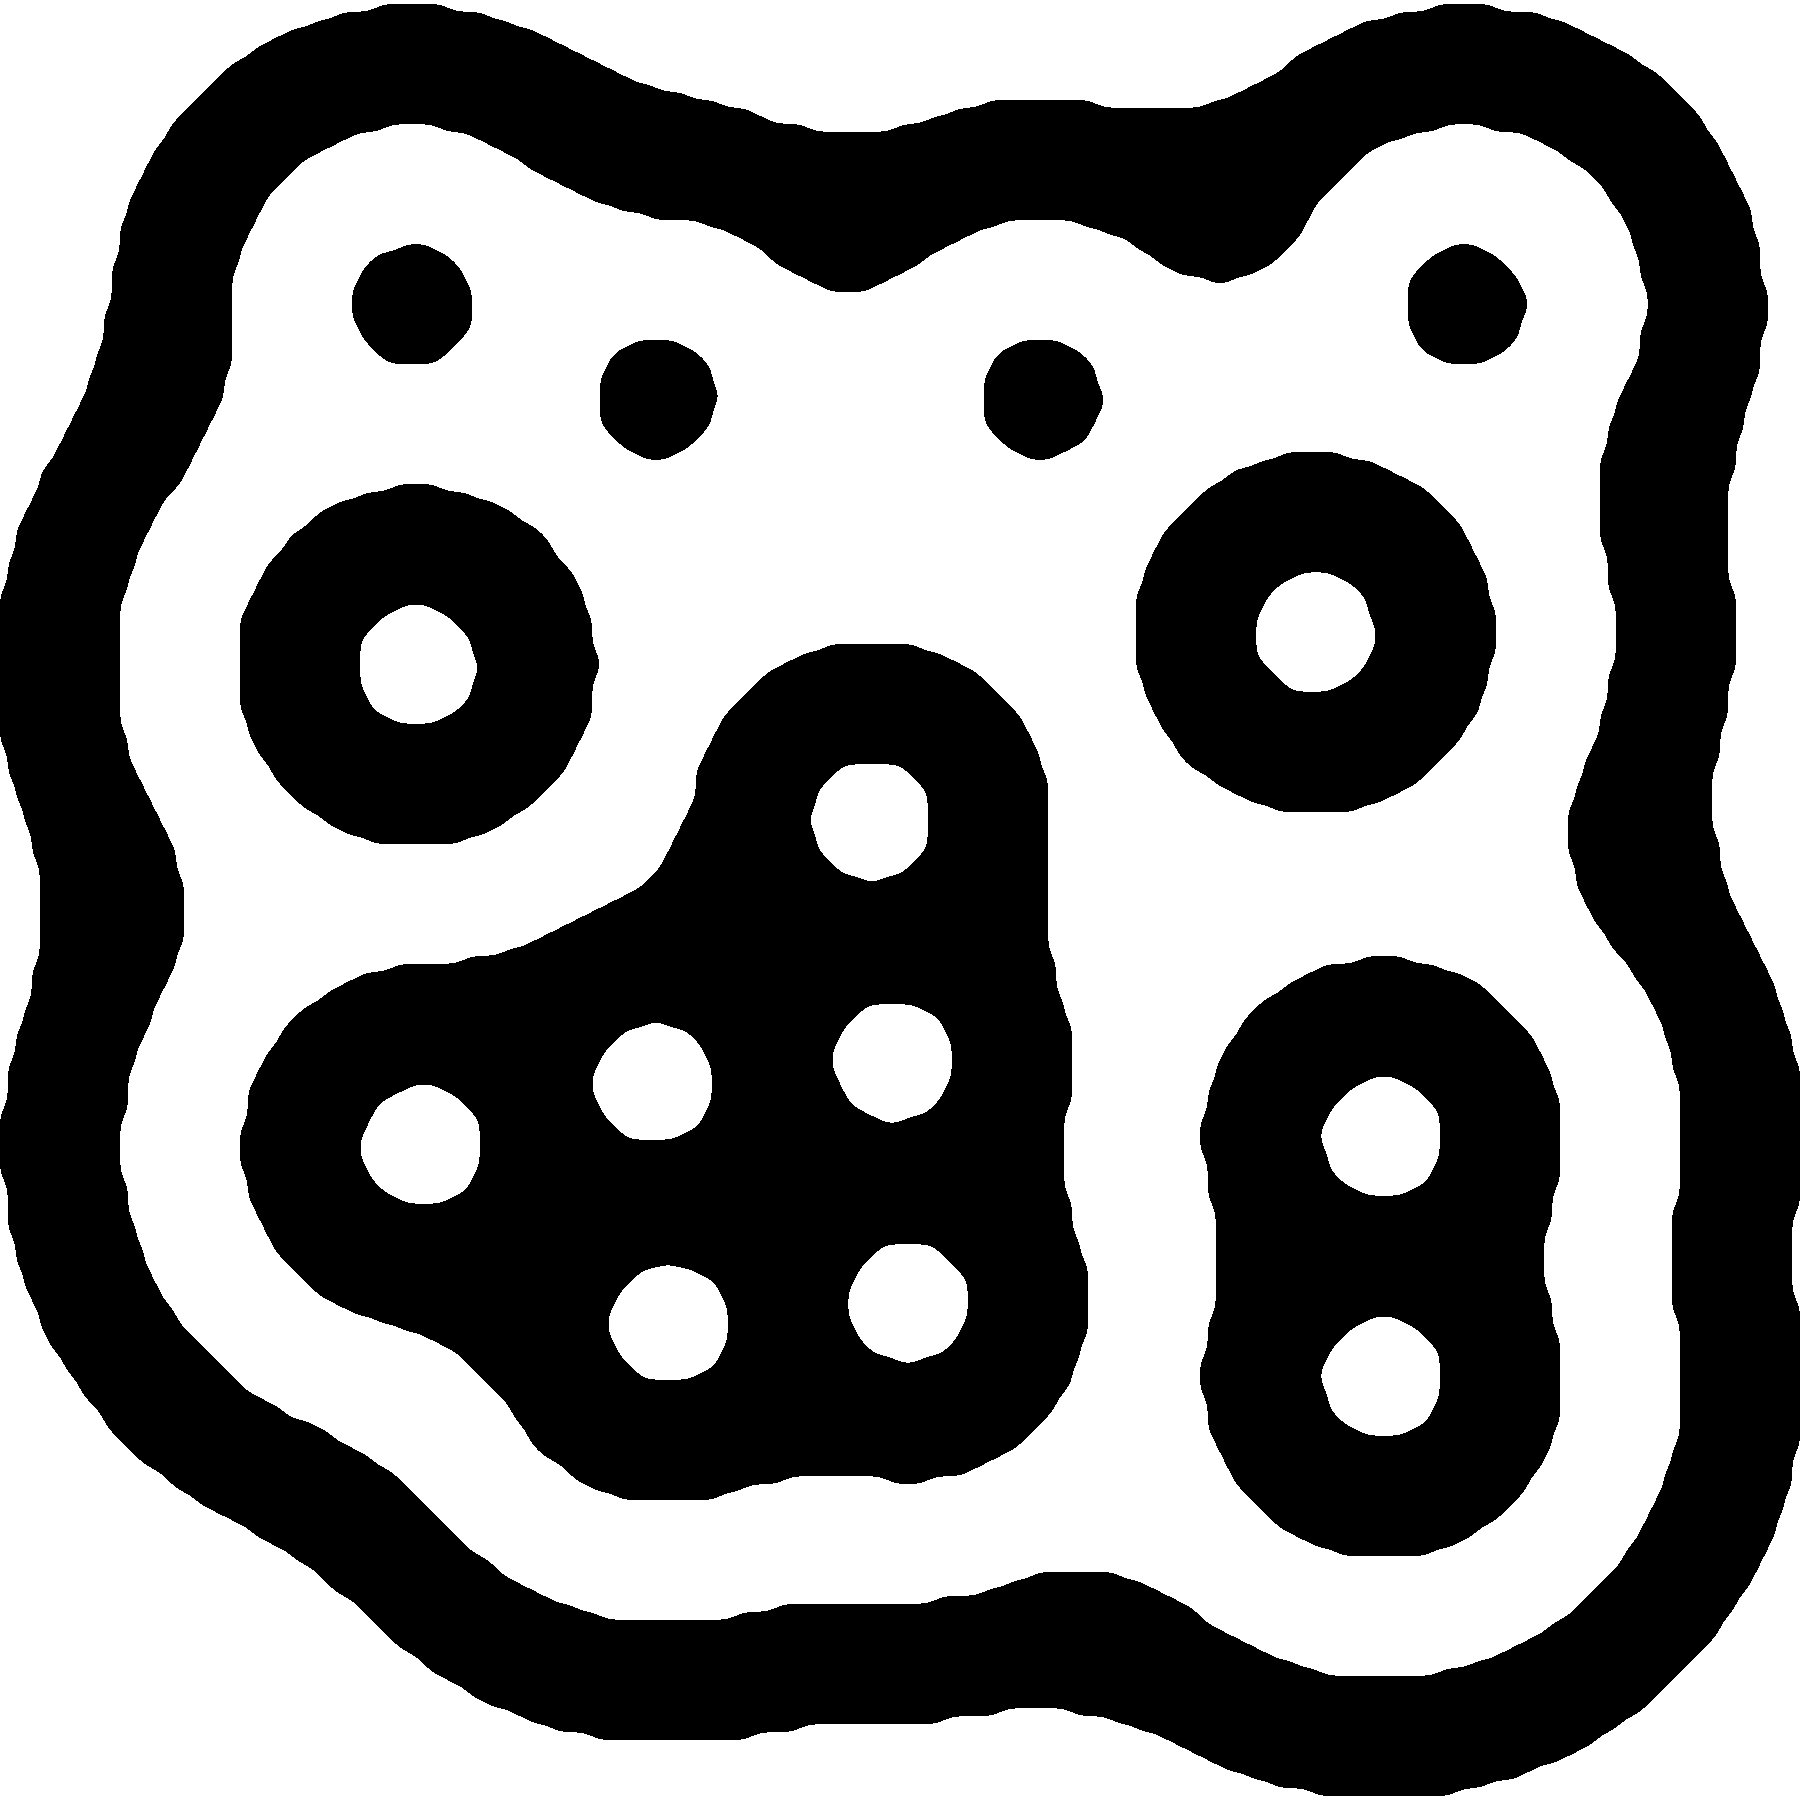
\includegraphics[height=1in]{img/ImplementierungInput/ReactivisionCode.png}
	\caption{ReacTIVision Code}
	\label{fig:img_ImplementierungInput_ReactivisionCode}
\end{figure}

Die ReacTIVision-Software ist plattformübergreifend für Windows, Linux und Mac OS X verfügbar. Sie greift über plattformspezifische Schnittstellen auf eine angeschlossene Kamera zu und wertet das empfangene Bild in Echtzeit aus. Dabei sind bei einer Kameraauflösung von 1024 x 768 Bildpunkten Bildraten von 15-20 Bildern pro Sekunde erreichbar. Diese Leistung wird auch durch eine höhere Anzahl von gleichzeitig im Bild vorhandenen Codes nicht merklich geringer.

Neben der Position der Codes wird auch deren aktuelle Rotation sowie die erste Ableitung dieser drei Parameter (also ein Maß für die Bewegung) extrahiert. Zudem können Finger, die die Oberfläche berühren, erkannt und deren Position extrahiert werden. Dies ist auch für mehrere Finger möglich, wobei eine eindeutige Zuordnung über die Zeit erhalten bleibt und so rudimentäre Multitouch-Funktionen umgesetzt werden können.

Als problematisch stellt sich wie auch bei allen anderen betrachteten optischen Ansätzen die Abhängigkeit der Erkennungsqualität von der Umgebungsbeleuchtung bzw. deren Änderung über die Zeit dar. ReacTIVision arbeitet mit adaptiven Filteralgorithmen zur Aufbereitung des Bildes, was jedoch nur leichte Beleuchtungsschwankungen ausgleichen kann. Die Software kann manuell an die Beleuchtungsverhältnisse angepasst werden (Einstellung der Blendenöffnung und der Bildverstärkung), bei sich ändernden Lichtverhältnissen muss jedoch regelmäßig eine Nachführung der Parameter vorgenommen werden.

Die aus dem Bilderstrom gewonnenen Daten werden im Falle einer Änderung zumindest eines Wertes über eine Netzwerkschnittstelle (UDP-basiert) in einem proprietären Protokoll zur Verfügung gestellt. Zu diesem Protokoll werden Schnittstellen und Referenzimplementierungen in unterschiedlichen Programmiersprachen -- unter anderem C(++) und Java -- zur Verfügung gestellt. Applikationen können diese Schnittstelle implementieren und werden mittels sechs zu implementierenden Methoden an die Erkennungsroutinen angebunden (je 3 für Code- und für Fingertracking).

% paragraph reactivision (end)
% subsubsection frameworks_für_video_basierten_input (end)
% subsection verfügbare_frameworks (end)

\subsection{Technologieentscheidung} % (fold)
\label{sub:technologieentscheidung}

Auf Basis der Anforderungen, die im Anwendungsfall an das Werkzeug gestellt werden, ist nun nach der grundsätzlichen Entscheidung für ein auf optischen Ansätzen basierenden System die Entscheidung für ein konkretes Framework zu treffen. 

\subsubsection{Vergleich der Frameworks für videobasierten Input}\label{subs:vergleich_video_frameworks}

Für die Anbindung von videobasiertem Input wurde drei Frameworks vorgestellt. Diese Frameworks sind nun hinsichtlich mehrere Aspekte zu vergleichen, die sich aus den Anforderungen der zu erstellenden Applikation sowie der Forderung nach möglichst einfacher (im Sinne von weniger aufwändig) Einbindung des Frameworks ergeben. Im Einzelnen sind dies 
\begin{itemize}
	\item die Unterstützung bei der Einbindung von Kameras und eine Schnittstelle zur Programmiersprache Java,
	\item eine stabile und in Echtzeit ablaufende Bilderkennung,
	\item eine ausreichende Anzahl von Codes (Größenordnung 100),
	\item die Extraktion von Position und Rotationsinformation für Codes im Erfassungsbereich der Kamera,
	\item die Art der Kopplung von Framework und darauf aufbauender Applikation, sowie
	\item die technische und lizenzrechtliche Möglichkeit, die Frameworks an die eigenen Anforderungen anzupassen.
\end{itemize}
    
ReacTIVision bietet die umfassendste Unterstützung zur Einbindung unterschiedlicher Videoquellen und ist zur Anwendungsseite hin durch die Netzwerkschnittstelle am flexibelsten einsetzbar. Alle drei Ansätze bieten Schnittstellen bzw. Konnektoren für die Programmiersprache Java an. Die Frameworks selbst sind in C(++) oder Java erstellt und können auf den gängigen Plattformen (Windows, Linux, Mac OS x) ausgeführt werden. Eine Verteilung der Applikation auf mehrere Rechner wird nur von ReacTIVision explizit unterstützt.

Hinsichtlich der eigentlichen Bilderkennungs-Routinen sind die Ansätze in ihrer Leistung und Geschwindigkeit vergleichbar, leiden aber alle unter der Abhängigkeit von der Umgebungsbeleuchtung. ReacTIVision bietet hier als einziger Ansatz die Möglichkeit, Kameraparameter zur Laufzeit nachzuführen und so Schwankungen der Umgebungshelligkeit auszugleichen.

Durch den eingesetzten Mapping-Ansatz sind AR Toolkit und ReacTIVision hinsichtlich Form und Inhalt der Codes flexibler als direkt codierende Ansätze wie Visual Codes. Dies ist im konkreten Anwendungsfall relevant, da aufgrund der Token-Form und deren beschränkter Größe eine ideale Platzausnutzung erfolgen muss, um ausreichende Erkennungsleistung zu gewährleisten.

Die Extraktion der Raumparameter (Neigungsinformation, ...), die von AR Toolkit und Visual Codes ermöglicht wird, ist bei tisch-basierten Werkzeugen wie dem hier vorgestellten nicht notwendig -- die Erhebung planarer Parameter (Position und Rotation) ist ausreichend. AR Toolkit liefert aufgrund seiner Ausrichtung auf Augmented Reality-Anwendung die Parameter in Form einer Transformationsmatrix, die für die Verarbeitung in 3D-Umgebungen wie OpenGL direkt geeignet ist, im hier verfolgten Ansatz jedoch einer zusätzlich Umrechnung auf das benötigte Parameterformat unterzogen werden müsste.

Die Anzahl der verfügbaren und zuverlässig unterscheidbaren Codes muss für die hier vorgeschlagene Anwendung in der Größenordnung 100 liegen. Visual Codes und ReacTIVision erfüllen diese Anforderung, AR Toolkit bietet im Lieferumfang weniger Codes an, diese können jedoch erweitert werden und bieten auch in der geforderten Anzahl noch ausreichend Unterscheidungsmerkmale für eine zuverlässige Unterscheidung \citep{Wagner03}.

Das AR Toolkit und Visual Codes müssen direkt über eine Einbindung von Bibliotheken in die eigene Applikation integriert werden. ReacTIVision ist hier flexibler und wird über einen Netzwerkport mit der Zielapplikation verbunden. Dies kommt dem hier verfolgten Ansatz entgegen, da ein verteilter Betrieb aufgrund der hohen Rechenanforderungen oder im Betrieb mit mehreren Ausgabegeräten notwendig werden kann.

Von AR Toolkit und ReacTIVision steht der Source-Code zur Verfügung. Lizenzrechtlich erlauben das AR Toolkit und ReacTIVision explizit eine Veränderung des Sourcecodes unter der GNU Public Licence\footnote{http://www.gnu.org/licenses/gpl-3.0.html} bzw. der Lesser GNU Public Licence\footnote{http://www.gnu.org/licenses/lgpl-3.0.html}. AR Toolkit verfolgt dabei einen Dual Licensing Ansatz, der einen kommerziellen Einsatz kostenpflichtig macht. Zu Visual Codes sind keine Lizenzinformationen erhältlich, auch der Sourcecode steht nicht zum Download bereit.

\begin{table}[htbp]
	\centering
	\caption{Gegenüberstellung der Frameworks für video-basierten Input}
	\begin{tabular}{| p{3cm} || p{3cm} | p{3cm} | p{3cm} |} \hline
		 & AR Toolkit & Visual Codes & ReacTIVision \\ \hline \hline
		Kamera\-unterstützung 		  		& nativ auf allen unterstützten Plattformen (Interfaces \& Features treiber-abhängig) & nativ nur für Mobiltelefone & nativ auf allen unterstützten Plattformen \\ \hline
		Plattformen 			  	  		&  Windows, Linux, Mac OS X  & Java-basiert auf allen Plattformen & Windows, Linux, Mac OS X \\ \hline
		Schnittstelle zu Java 		  		& via Drittanbieter-Software & nativ & ja \\ \hline
		Stabilität der Bilderkennung 	  	& abhängig von den verwendeten Markern & eher hoch & hoch \\ \hline
		Kompensations\-möglichkeit bei schlechten Lichtbedingungen & nein & nein & ja \\ \hline
		Geschwindigkeit der Bilderkennung 	& > 10 fps & > 10 fps & > 10 fps \\ \hline
		Anzahl von gleichzeitig erkennbaren Codes 		  			& keine Einschränkung & keine Einschränkung & keine Einschränkung \\ \hline
		Erkennung von Position 		  		& implizit & ja & ja \\ \hline
		Erkennung von Rotation 				& implizit & ja & ja \\ \hline
		Kopplung von Framework und Applikation & eng & eng & lose \\ \hline
		Source-Code verfügbar 			  	& ja & nein & ja \\ \hline
		Lizenz 				 				& GPL, alternativ kommerziell & unbekannt & GPL, LGPL \\ \hline
	\end{tabular}
	\label{tab:videobasierterInput}
\end{table}

Auf Basis der in Tabelle \ref{tab:videobasierterInput} angegeben Gegenüberstellung ist erkennbar, dass das ReacTIVision-Framework für den hier verfolgten Ansatz am besten geeignet erscheint. Betrachtet man die funktionalen Anforderungen, erscheinen zwar alle Frameworks grundsätzlich geeignet, die nicht-funktionalen Anforderungen -- vor allem die plattform-übergreifende Einsetzbarkeit, die Möglichkeit zum verteilten Betrieb und die gute Unterstützung beliebiger Kameras sowie deren Konfigurierbarkeit -- sprechen für die ReacTIVision-Plattform. Diese wird deshalb zur Umsetzung des Werkzeugs verwendet. Der zusätzliche Einsatz eines generischen Frameworks zur Flexibilisierung der Applikationsstruktur ist damit nach wie vor möglich und wird im nächsten Abschnitt diskutiert.

% subsubsection vergleich_video_frameworks (end)

\subsubsection{Vergleich der generischen Frameworks}\label{subs:vergleich_generische_frameworks}

Der Einsatz eines generischen Frameworks ist im konkreten Anwendungsfall für die Modularisierung der Interpretations- und Output-Module denkbar. Eine weitere Anwendung von generischen Frameworks ist die Sicherstellung der Skalierbarkeit der Anzahl der Ausgabemodule ggf. auch während des Betriebs der Applikation (um z.B. weitere Viewer-Module zur Beobachtung des Modellierungsvorganges während der Laufzeit zuschalten zu können). Die Aspekte die beim Vergleich der vorgestellten Ansätze berücksichtigt werden müssen, sind deshalb
\begin{itemize}
  	\item die Unterstützung von modularen funktionalen Einheiten sowie
	\item die Möglichkeit diese zur Laufzeit zu laden und entfernen und
	\item die Konfigurierbarkeit der Verknüpfungen dieser Module.
\end{itemize}  
Daneben sind nicht-funktionale Anforderungen wie 
\begin{itemize}
	\item Skalierbarkeit,
	\item Effizienz bei der Weiterleitung und Verteilung der Anwendungsdaten und  
	\item die Lizenzbestimmungen des Frameworks
\end{itemize}  
zu berücksichtigen.

Die Modularisierung der Applikation wird von allen vier vorgestellten Frameworks unterstützt. Das Context Toolkit, Papiermaché und TUIpist unterscheiden dabei konzeptionell zwischen unterschiedlichen Arten von von Modulen (im Wesentlichen „Input“, „Verarbeitung“ und „Output“), das SiLiCon Context Framework unterscheidet nicht zwischen unterschiedlichen Modultypen, dort wird die Rolle eines Moduls ausschließlich über seine Attribute (also die nach außen sichtbaren funktionalen Einheiten) definiert. 

Eine Erweiterbarkeit der Applikation zur Laufzeit ist nur beim SiLiCon Context Framework und bei TUIpist möglich. Das SiLiCon Context Framework arbeitet hier mit eigens erstellten Java-Classloadern, die das Nachladen von Klassen (Modulen) und deren Integration in die Infrasturktur erlauben. TUIpist verwendet die inhärent dynamische Erweiterbarkeit des Java Jini Frameworks \citep{Arnold99}, auf Basis dessen es implementiert wurde. Das Context Toolkit und Papiermaché erlauben kein Nachladen oder Entfernen funktionaler Einheiten während der Laufzeit.

Die Konfiguration der Verbindungen zwischen den Modulen ist bei allen Frameworks möglich, konzeptionell jedoch unterschiedlich ausgeführt. Im Context Toolkit und in Papiermaché muss die Verbindung direkt im Programmcode codiert werden und wird im wesentlichen auf Methodenaufrufe abgebildet. Das SiLiCon Context Framework verwendet ereignisbasierte Regeln, um Module zu verknüpfen. Ein von einem Modul ausgelöstes Ereignis kann hier (ggf. durch Bedingungen eingeschränkt) Aktionen in anderen Modulen auslösen. Eine Besonderheit dieses Ansatzes ist, das Teile der Interpretationslogik (also der Erkennung von Benutzerinteraktion aus den Rohdaten) in die Regeln ausgelagert werden und damit jederzeit dynamisch verändert werden können. So kann zum Beispiel die Interpretation der Nähe zwischen zwei Token in einer Regel codiert werden und so in die Reihe der zulässigen (bzw. erkennbaren) Interaktionen aufgenommen werden. TUIpist benötigt hingegen keinerlei explizite Verbindung der Module, da sämtliche Koordination über den geteilten Datenraum ausgeführt wird. Die Verknüpfungslogik wird hier in die Module verschoben, die selbst wissen müssen, für welche Daten für sie ggf. relevant sind und welche sie deshalb dem Tuplespace entnehmen.

Hinsichtlich der Skalierbarkeit der Frameworks können aufgrund mangelnder Vergleichsdaten keine fundierten Aussagen getroffen werden. Hinzuweisen ist jedoch auf die Unterstützung von verteiltem Betrieb einer Applikation durch das SiLiCon Context Framework (via SOAP-Aufrufe \citep{Curbera02} und das TUIpist Framework (via Jini und Java \gls{RMI} \citep{Downing98}). Durch diese Verteilbarkeit ist kann die Problematik mangelnder Rechenressourcen umgangen werden, die vor allem bei rechenintensiven Anwendungen wie der eingesetzten Bildanalyse im optischen Tracking auftritt.

Die Beurteilung der Effizienz der Frameworks ist hier in Hinblick auf die geforderte Echtzeit-Interaktion mit dem System als relevant zu erachten. Das Haupt-Kriterium für Effizienz ist dementsprechend die Verzögerung zwischen Eingabe-Ereignissen und dem Feedback auf Applikationsebene, die beim Einsatz der Frameworks auftritt. Eine Beurteilung in absoluten Zahlen kann hier mangels entsprechenden Datenquellen ebenfalls nicht erfolgen, konzeptionell sind aber bei den Frameworks, in denen Module direkt durch Programm-Code verknüpft werden (Context Toolkit und Papiermaché), eher geringe Verzögerungen zu erwarte. Die beiden Frameworks, die mit expliziter und konfigurierbarer Middleware zur Datenvermittlung arbeiten (SiLiCon Context Framework und TUIpist) lassen eher höhere Verzögerungen erwarten, wobei der ereignisbasierte Ansatz des SiLiCon Context Framework dem daten-basieren Ansatz von TUIpist insofern überlegen ist, als das bei der datenbasierten Interaktion die Module in regelmäßigen Intervallen nach neuen Daten suchen müssen (Polling, „Information Pull“-Ansatz), während bei ereignisbasierten Ansätzen die Benachrichtigung der betroffenen Module automatisch und zum Zeitpunkt des Auftretens des Ereignisses erfolgt („Information Push“-Ansatz). Der Information Pull-Ansatz sorgt dabei einerseits für erhöhten Kommunikationsaufwand und potentiell für Verzögerungen bei Ereignissen, die innerhalb eines Polling-Intervalls auftreten.

\begin{table}[htbp]
	\centering
	\caption{Gegenüberstellung der generischen Frameworks}
	\begin{tabular}{| p{3cm} || p{2cm} | p{2cm} | p{2cm} | p{2cm} |} \hline
		 & Context Toolkit & SiLiCon Context Framework & Papiermaché & TUIpist \\ \hline \hline
		Modularität & ja & ja & ja & ja \\ \hline
		Erweiterbarkeit zur Laufzeit & nein & ja & nein & ja \\ \hline
		dynamisch konfigurierbare Orchestirierung & nein & ja & nein & ja \\ \hline
		Skalierbarkeit & schlecht & gut & schlecht & sehr gut \\ \hline
		Effizienz bei der Weiterleitung von Daten & sehr gut & gut & sehr gut & ausreichend \\ \hline
		Lizenz & unbekannt & unbekannt & Open-Source (nicht näher bestimmt) & Eigen\-entwicklung \\ \hline
	\end{tabular}
	\label{tab:generischeFrameworks}
\end{table}

Auf Basis der in Tabelle \ref{tab:generischeFrameworks} angegebenen Gegenüberstellung erscheinen das SiLiCon Context Framework und TUIpist als die beiden geeignetsten Kandidaten für den Einsatz als generisches Framework im hier vorgestellten Anwendungsfall. Das Context Toolkit und Papiermaché scheiden aus verschiedenen Gründen, vor allem aufgrund der mangelnden Flexibilität aus.

Stellt man die beiden verbleibenden Frameworks gegenüber, so sind hinsichtlich der funktionalen Anforderungen keine Vorteile für einen der beiden Kandidaten zu identifizieren. Hinsichtlich der nichtfunktionalen Anforderungen scheint TUIpist hinsichtlich der Skalierbarkeit leichte Vorteile zu haben, da das Nachladen von neuen Instanzen weniger Aufwand versacht als im Fall des SiLiCon Context Framework (lediglich Laden eines Moduls im ersten Fall gegenüber Laden und Einbinden über eine Änderung der Regelbasis im zweiten Fall). Außerdem ist die technologische Basis der Verteilungsarchitektur in TUIpist konzeptionell auf höherer Ebene angesiedelt und mächtiger in der Verwaltung der Applikationsstruktur (unter anderem werden neue Module bei TUIpist automatisch in die Infrastruktur eingebunden, sobald sie angemeldet werden, im SiLiCon Context Framework muss für jeden Kommunikationskanal die IP-Adresse des Empfängers bekannt sein und in die Regelbasis aufgenommen werden). 

Hinsichtlich der Effizienz der Kommunikation bietet das SiLiCon Context Framework gegenüber TUIpist aus den oben beschriebenen Gründen (Benachrichtung über Änderungen gegenüber Polling) Vorteile. Für die hier beschriebene Applikation fällt die Entscheidung trotzdem zugunsten TUIpist. Neben der generell weniger aufwändigen Konfiguration kommt die Struktur von TUIpist einem iterativen Software-Entwicklungsprozess insofern eher entgegen, als dass die Modularisierung von initialen, monolithischen Prototypen (z.B. basierend auf der Struktur des zuvor ausgewählten ReacTIVision-Frameworks) einfacher möglich ist. Dies liegt darin begründet, dass in der modularen und dynamischen Struktur von TUIpist die gesamte Applikationslogik in den Modulen enthalten ist und so Teile aus einer monolithischen Applikation herausgelöst und direkt übernommen werden können, wobei lediglich die Logik der Datenübergabe von direkten Methoden-Aufrufen auf die TUIpist-Routinen zum Zugriff auf den Tuplespace umgearbeitet bzw. erweitert werden muss. Beim korrekten Einsatz des SiLiCon Context Framework wandert wie oben beschrieben ein Teil der Applikationslogik in die Regelbasis, was erhöhten Aufwand bei der iterativen Entwicklung verursacht und außerdem das Zusammenspiel der Applikations-Module unübersichtlicher und schwerer fassbar macht.

% subsubsection vergleich_generische_frameworks (end)

% subsection technologieentscheidung (end)
% section möglichkeiten_zur_erfassung_von_benutzerinteraktion (end)

\section{Konzeption und Umsetzung der Hardwarekomponenten} % (fold)
\label{sec:konzeption_und_umsetzung_der_hardwarekomponenten}

Basierend auf der oben getroffenen Technologieentscheidung zugunsten eines optischen, video-basierten Input-Systems für das hier zu erstellende Tabletop Interface wird in diesem Abschnitt das konkrete Hardware-Design beschrieben. Dies umfasst die Beschreibung des Tabletop Interfaces im Überblick und detaillierte Betrachtungen des Token-Designs sowie der Tisch-Oberfläche, die als Input-Kanal dient. Weiters werden spezifische Herausforderungen und der jeweilige hier verfolgte Lösungsansatz beschrieben. Nicht Gegenstand dieses Abschnitts sind jene Hardware-Komponenten, die für die Ausgabe von Information eingesetzt werden. Obwohl hier im Überblick angeführt, werden sie detailliert erst in Kapitel XY über die Visualisierung der Modellierungsinformation beschrieben.

\subsection{Überblick} % (fold)
\label{sub:Überblick}

Das Tabletop Interface ist als Tisch mit einer Oberfläche von 100 cm x 80 cm ausgeführt. Die Höhe beträgt 110 cm. Die wesentlichen Hardwarekomponenten sind die Tischoberfläche, die in semi-transparentem Acrylglas ausgeführt ist und die Bodenplatte, in die die Kamera zum optischen Tracking der Tokens auf der Oberfläche sowie der Videoprojektor zur Ausgabe von Information auf der Oberfläche (Projektion von unten) eingebaut sind (siehe Abbildung \ref{fig:img_ImplementierungInput_TischSeitenansicht}). Der Tisch ist auf allen Seitenflächen mit Platten aus expandiertem Polystyrol (Styropor) verkleidet, um im Inneren kontrollierte Umgebungslichtbedingungen für die Bilderfassung mit der Kamera zu schaffen. Die kontrollierten Bedingungen werden durch den Einsatz von vier Beleuchtungsmodulen gewährleistet, die ebenfalls in der Bodenplatte integriert sind und über den Seitenflächen eingebaute Streuscheiben für eine einheitliche, diffuse Beleuchtung der Tischinnenraums sowie der Oberfläche sorgen.

\begin{figure}[htbp]
	\centering
		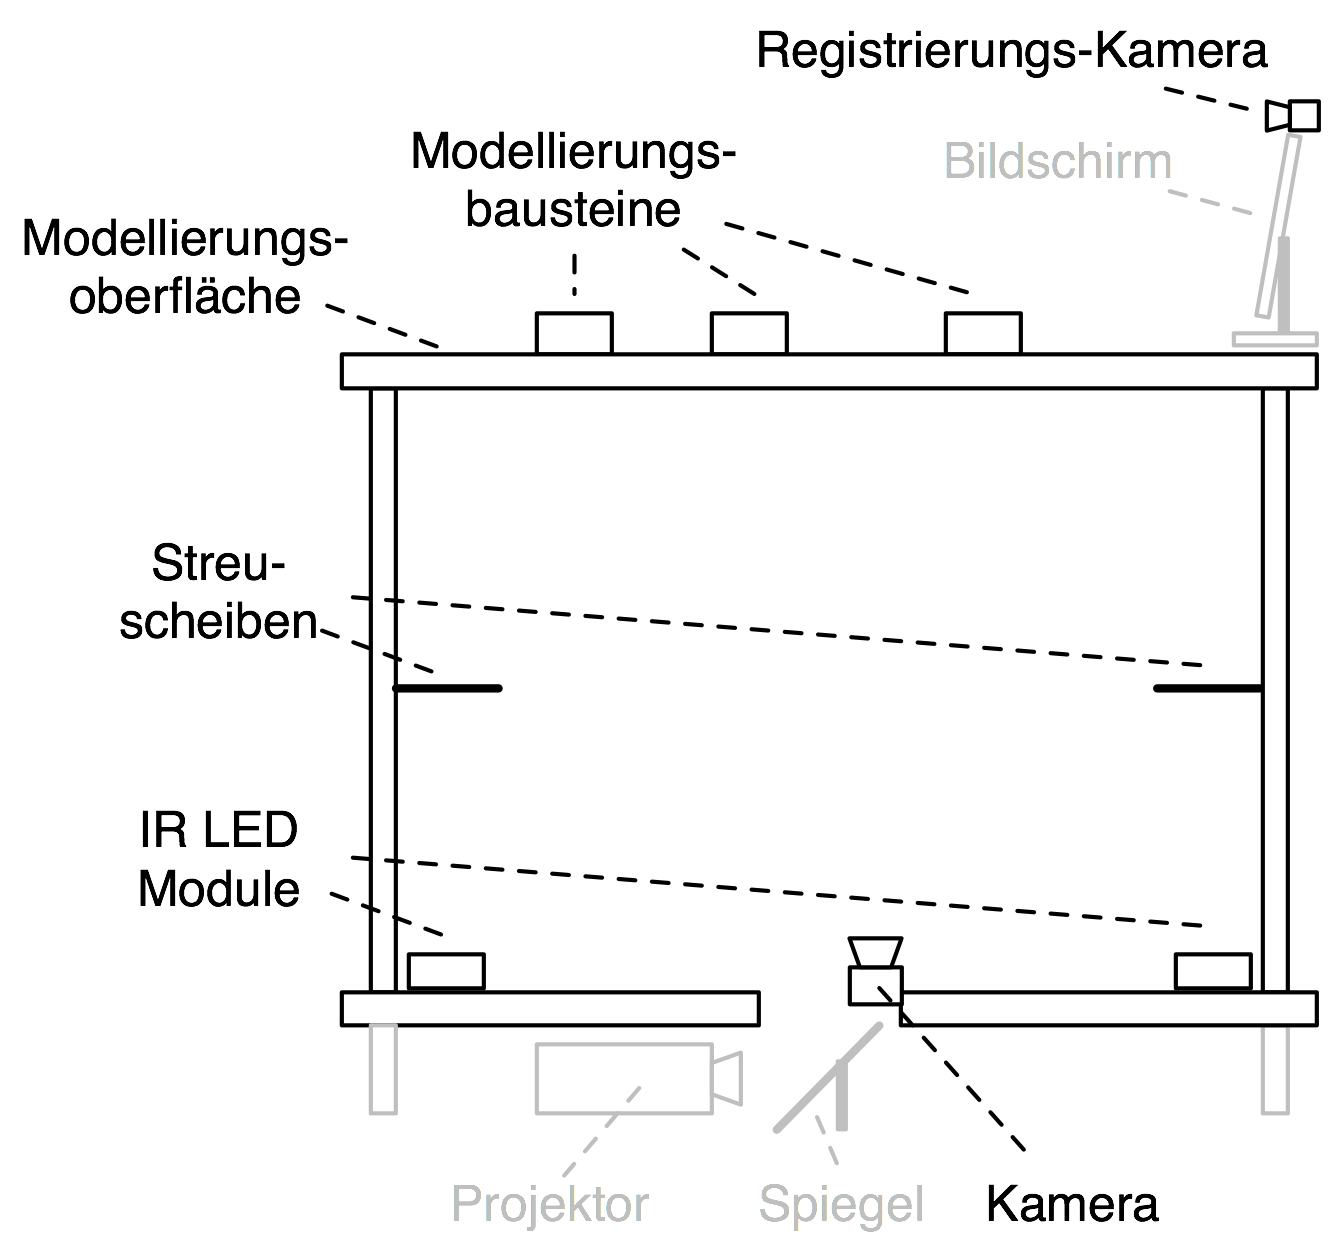
\includegraphics[height=3in]{img/ImplementierungInput/TischSeitenansichtInput.png}
	\caption{Überblick über den Aufbau des Werkzeugs -- Eingabekomponenten}
	\label{fig:img_ImplementierungInput_TischSeitenansicht}
\end{figure}

Am Tisch befindet sich zusätzlich ein Bildschirm, auf dem entsprechend der Anforderungen zur Unterstützung der Modellierung Zusatzinformation ausgegeben wird. Eine zweite Kamera, die am Bildschirm sitzt und der unterstützenden Erfassung von Information dient (zum Beispiel der bereits erwähnten Registrierung von geschachtelten Tokens).

Das gesamte System ist so zerlegbar, dass es im Kofferraum eines Mittelklassewagens transportiert werden kann. Es werden dazu die Verkleidungsplatten und Tischbeine entfernt, die Tischplatte kann dann direkt auf die Bodenplatte gesetzt und verbunden werden. Das Volumen reduziert sich dabei auf 100 cm x 80 cm x 20 cm, wobei die Tischbeine, die Verkleidungsplatten und der Videoprojektor separat transportiert werden müssen. Ein Zusammenbau des Systems inklusive {K}alibrierung der Eingabe- und Ausgabe-Kanäle ist in etwa 30 Minuten möglich.

% subsection Überblick (end)

\subsection{Tokens und Input-Werkzeuge} % (fold)
\label{sub:tokens_&_input_werkzeuge}

In diesem Abschnitt werden die einzelnen durch die Benutzer manipulierbaren Token-Arten beschrieben. Neben den eigentlichen Modellierungstokens sind dies die Tokens zur Einbettung in Container sowie die Werkzeugtokens, von denen es Ausführungen zur Manipulation des Modells und Tokens zur Auslösung bzw. Kontrolle spezifischer Funktionalitäten gibt.

\subsubsection{Modellierungs-Tokens} %fold 
\label{subs:modellierungs_tokens}

Die eingesetzten Modellierungs-Tokens sind aus nicht transparentem Acrylglas gefertigt. Ihre Außenmaße betragen in etwa (je nach Form) 10 cm x 6 cm in der Grundfläche und 4 cm in der Höhe. Damit ist einerseits eine ausreichende Größe zur Anbringung der ReacTIVision-Codes gewährleistet, andererseits sind noch klein genug, um in einer Hand gehalten und manipuliert werden zu können. Die Codes werden auf der Unterseite der Tokens angebracht und auch von unten erfasst (siehe nächster Abschnitt), um eine Verdeckung der Codes während der Manipulation zu verhindern (siehe Abbildung \ref{fig:img_ImplementierungInput_TokensCodes}).

\begin{figure}[htbp]
	\centering
		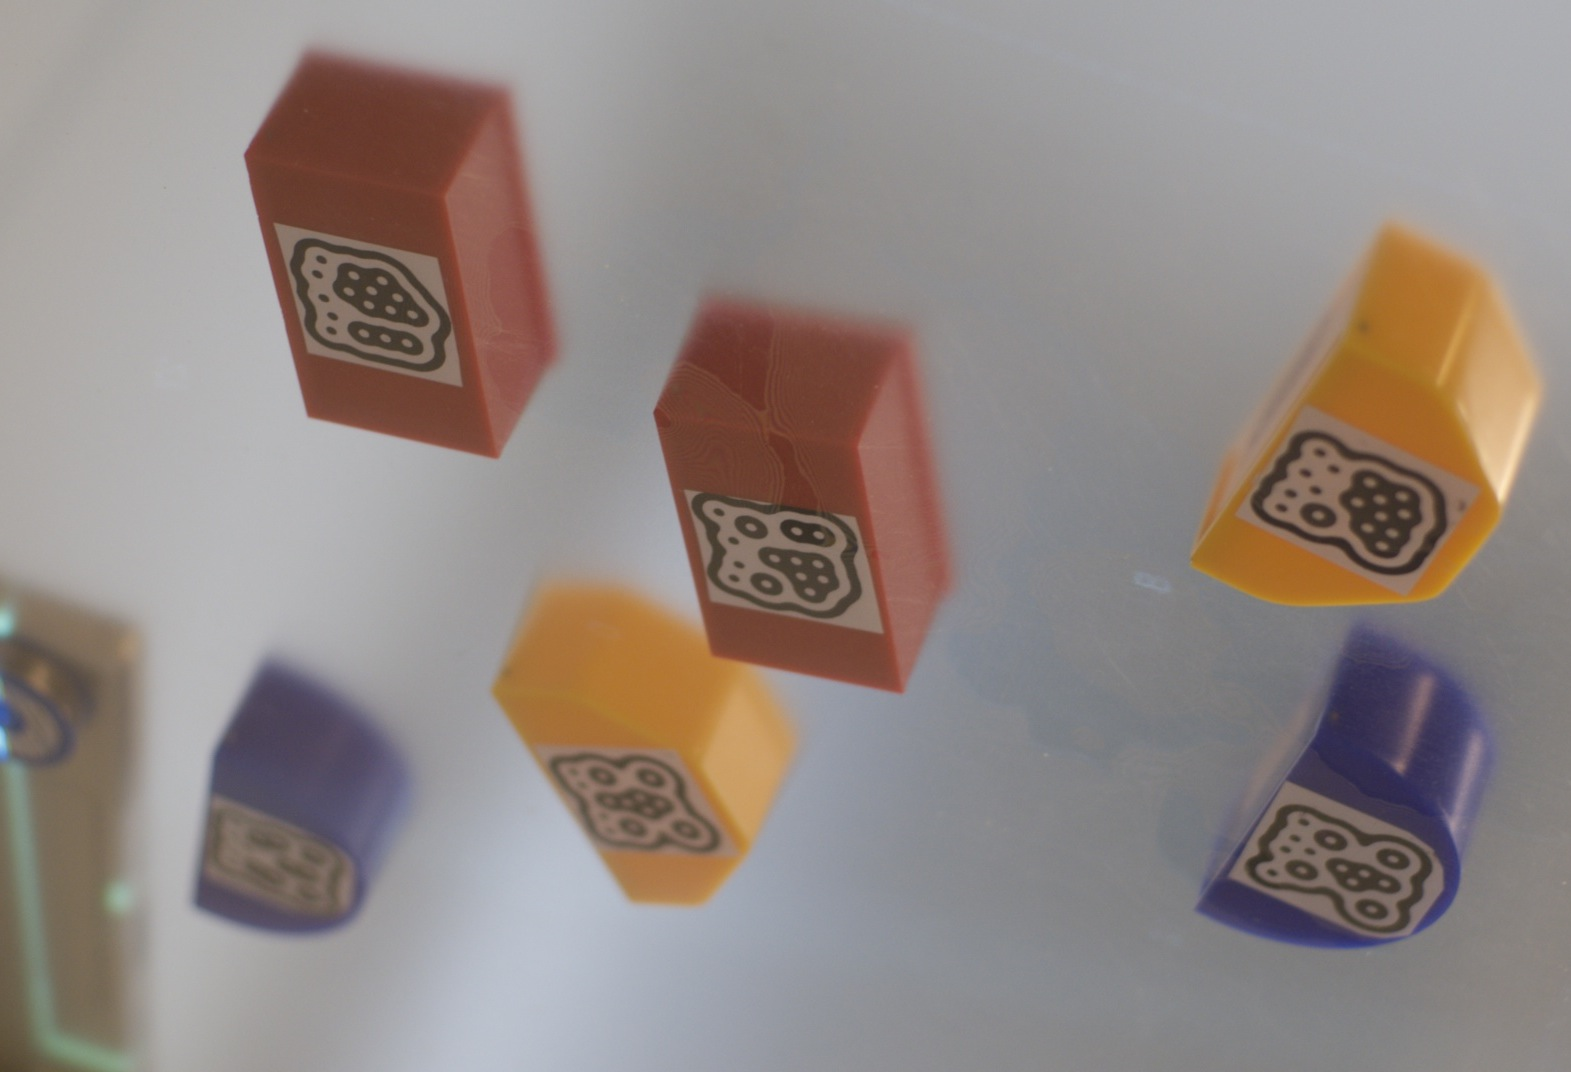
\includegraphics[height=2in]{img/ImplementierungInput/TokensCodes.jpg}
	\caption{An Tokens angebrachte ReacTIVision-Codes zur Identifikation}
	\label{fig:img_ImplementierungInput_TokensCodes}
\end{figure}

\begin{figure}[htbp]
	\centering
		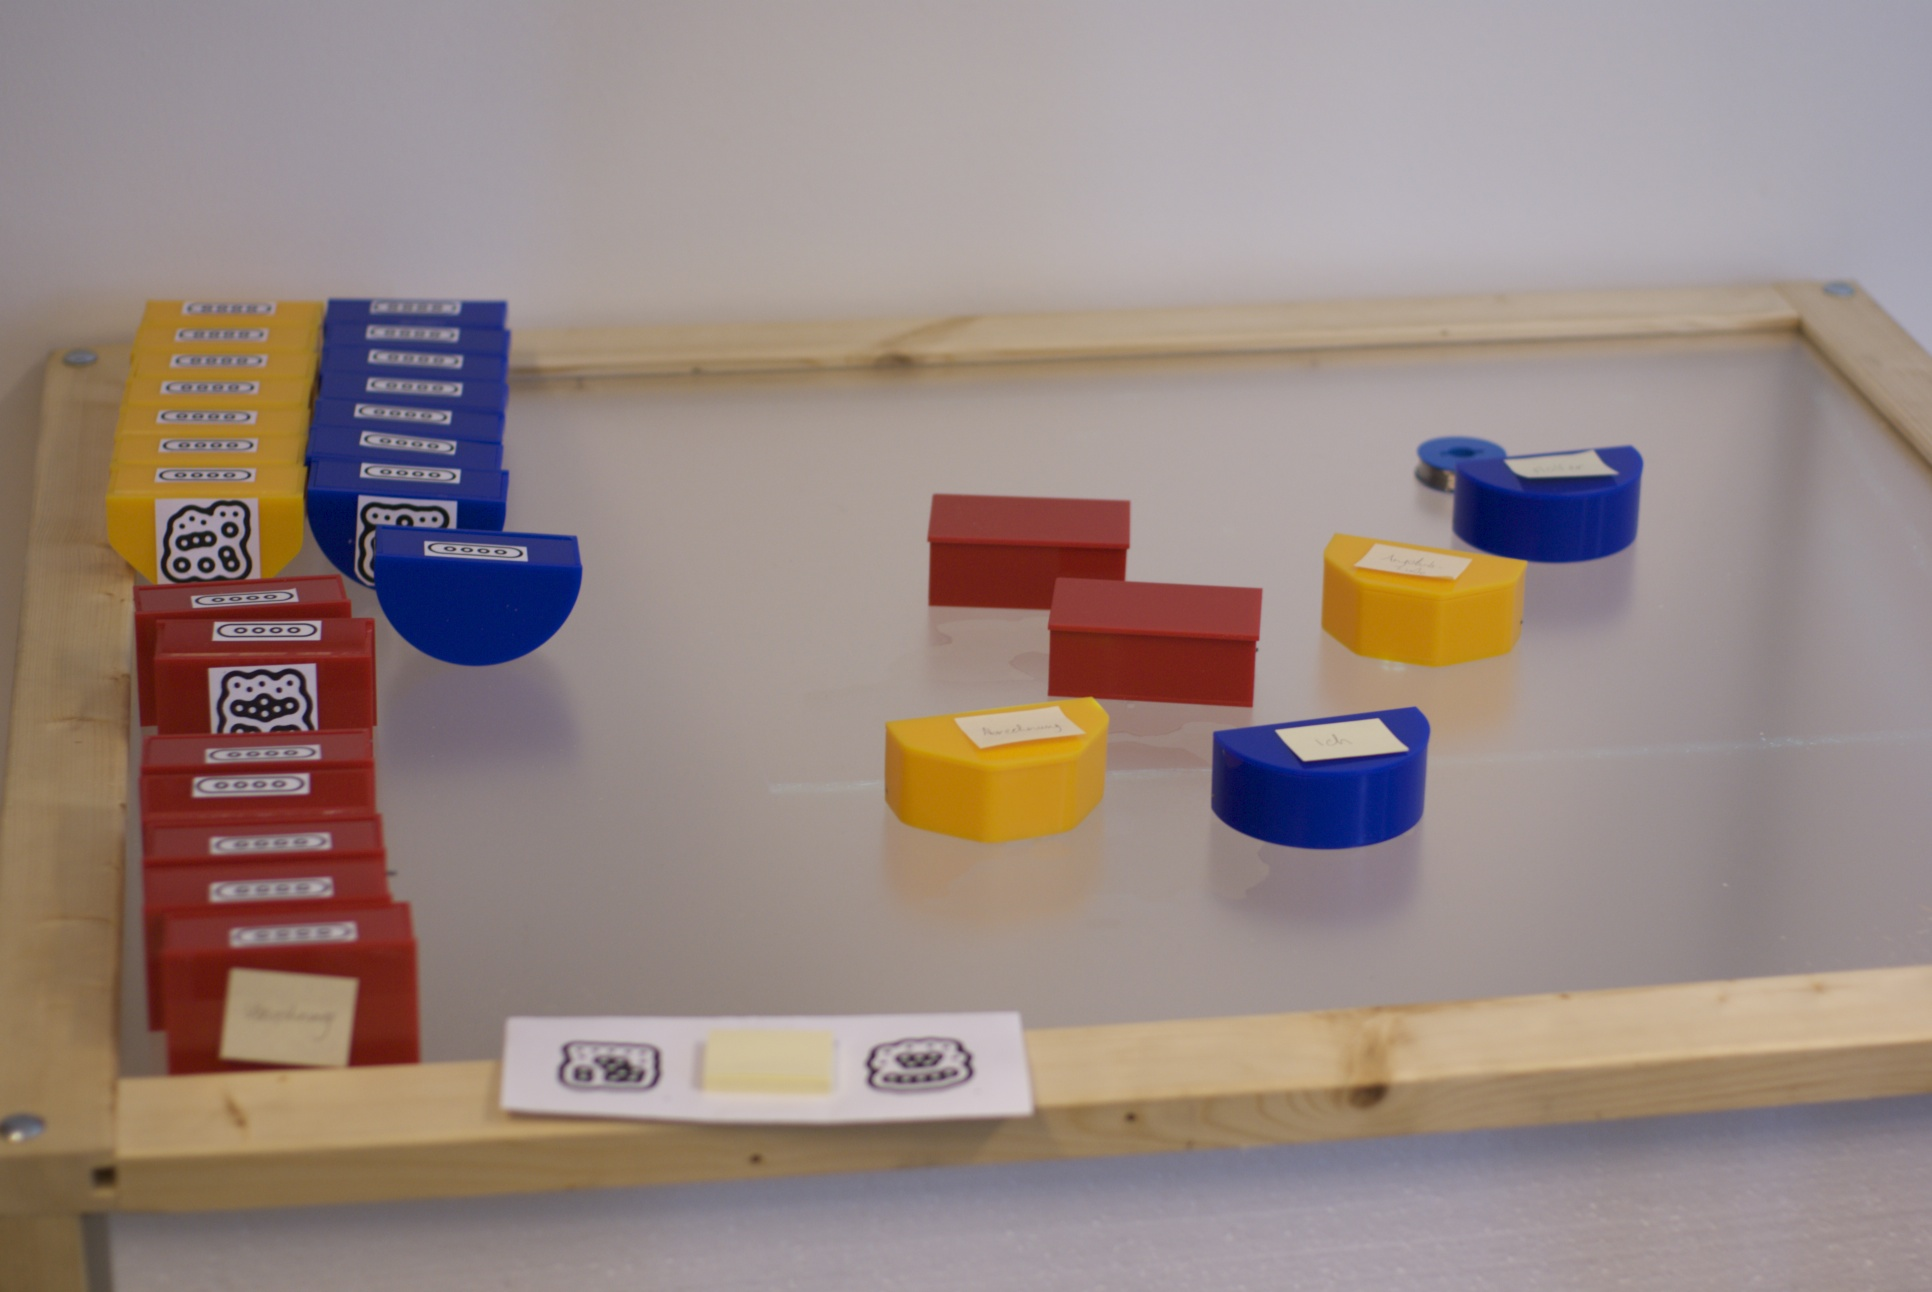
\includegraphics[height=2in]{img/ImplementierungInput/TokenTypes.jpg}
	\caption{Arten von Modellierungstokens}
	\label{fig:img_ImplementierungInput_TokenTypes}
\end{figure}


Die Modellierungs-Tokens wurden in drei Ausführungen gefertigt (siehe Abbildung \ref{fig:img_ImplementierungInput_TokenTypes}). Diese unterscheiden sich in Form und Farbe und können während der Modellierung von den Benutzern frei mit Bedeutung belegt werden. Die Auswahl der Formen und Farben erfolgte inspiriert von den Symbolen gängiger Modellierungsnotationen in Abstimmung mit fertigungstechnischen Einschränkungen. Eine Untersuchung geeigneter Token-Formen und eine auf diesen Ergebnissen basierende Umsetzung wurde nicht vorgenommen. Die liegt vor allem in der Tatsache begründet, dass sich der Fokus der hier vorgestellten Arbeit im Entwicklungsprozess von einem Werkzeug zur Geschäftsprozessmodellierung (mit vorgegebener Notation) hin zu einem allgemeiner einsetzbaren Werkzeug zur generischen Modellierung konzeptioneller Modelle (ohne vorgegebene Notation) entwickelte. Die Auswahl der Token-Formen fiel in die erste Phase, wodurch die Tokens im äußeren Erscheinungsbild an gängige Notationen zur Ablauf-Modellierung angelehnt sind. Die Token-Form scheint aber bei Benutzern ohne Modellierungs-Vorbildung geringen bis keinen Einfluss auf den Modellierungsprozess zu haben (siehe Kapitel XY -- Evaluierung).

\begin{figure}[htbp]
	\centering
		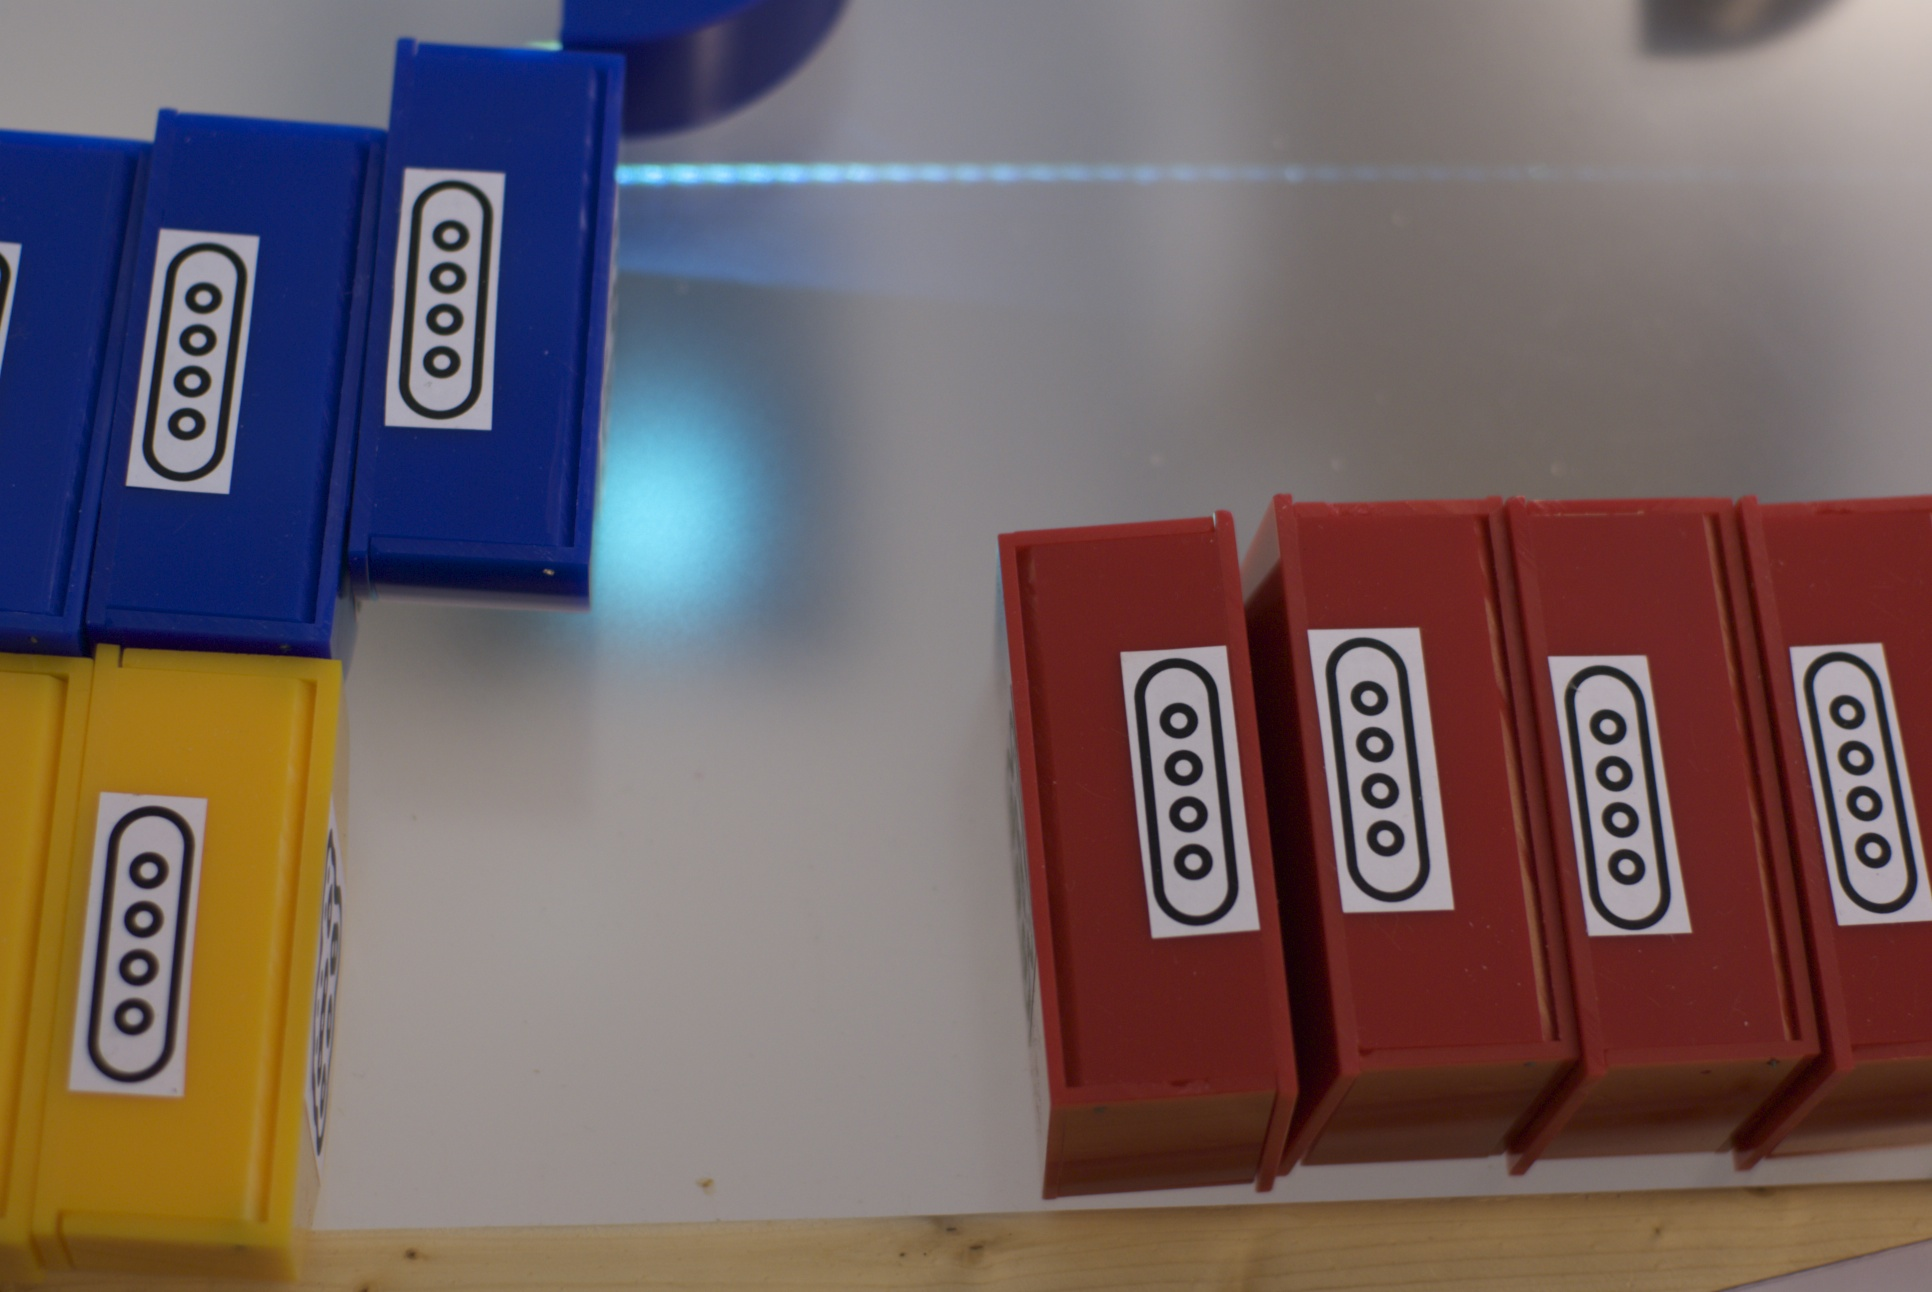
\includegraphics[height=2in]{img/ImplementierungInput/ContainerRueckseite.jpg}
	\caption{Rückwand von Container Tokens}
	\label{fig:img_ImplementierungInput_ContainerRueckseite}
\end{figure}

Wie in der Beschreibung der Anforderungen gefordert und oben bereits beschrieben, sind die Modellierungs-Tokens als Container ausgeführt. Im Abschnitt \ref{ssub:tokenzustand} über die Erkennung des Token-Zustands wurde beschrieben, das beim Einsatz von optischem Tracking eine Möglichkeit geschaffen werden muss, im Kamerabild zu erkennen, ob ein Token geöffnet ist oder nicht. Um den durchgängigen Einsatz des Erkennungsframeworks (ReacTIVision) zu gewährleisten, wird zu diesem Zweck ein zweiter Code eingesetzt (siehe Abbildung \ref{fig:img_ImplementierungInput_ContainerRueckseite}), der nur dann für die Kamera sichtbar wird, wenn das Token geöffnet ist. Hardwareseitig ist dies so umgesetzt, das die Modellierungstokens einen Öffnungsmechanismus besitzen, dessen Schanier nicht am Deckel sitzt (und damit nur diesen beweglich machen würde), sondern an der Bodenplatte, wodurch sich beim Öffnen eines Containers nicht nur der Deckel sondern auch die Hinterwand des Tokens bewegt (siehe Abbildung \ref{fig:img_ImplementierungInput_ContainerToken}). Die Hinterwand kommt im geöffneten Zustand auf der Oberfläche des Tisches zu liegen, wodurch der auf ihr angebrachte zweite Code für die Kamera sichtbar wird. So kann durch das an sich zur Positionsbestimmung eingesetzte optische Trackingsystem zuverlässig auch den Öffnungs-Zustand der Tokens auf der Oberfläche erkennen.

\begin{figure}[htbp]
	\centering
		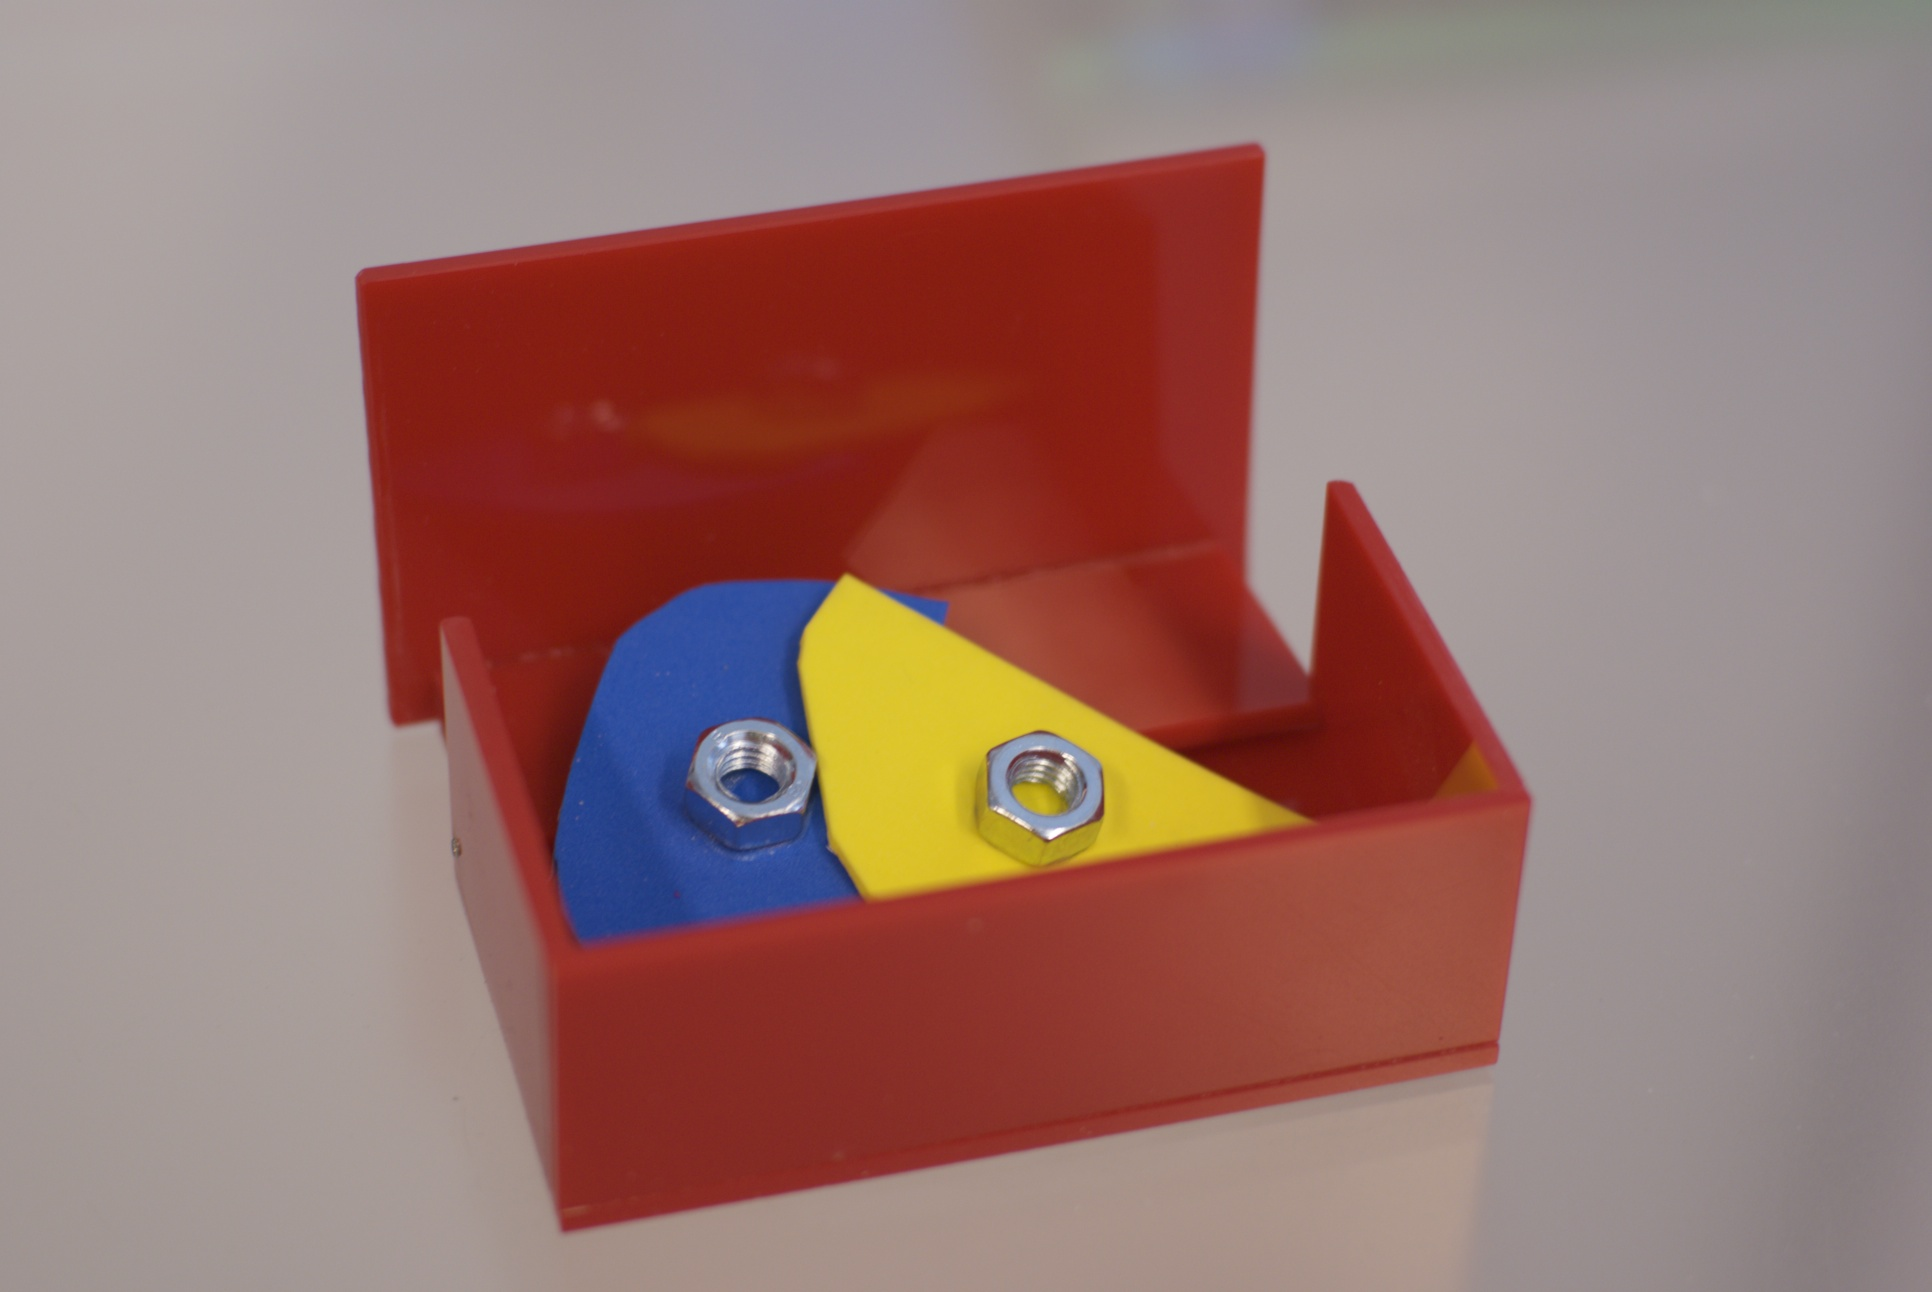
\includegraphics[height=2in]{img/ImplementierungInput/ContainerToken.jpg}
	\caption{Geöffnetes Container Token}
	\label{fig:img_ImplementierungInput_ContainerToken}
\end{figure}

Konzeptuell sind bei der Beschreibung der Verwendung dieser Tokens verschiedene Ebenen zu unterscheiden, die klar voneinander abgegrenzt werden müssen und in denen deshalb unterschiedliche Bezeichnungen verwendet werden. Diese Ebenen und die Beziehungen zwischen diesen sind in Abbildung \ref{fig:img_ImplementierungInput_ElementTaxonomie} in Form einer einfachen Taxonomie dargestellt. Als „\emph{Modellelement}“ wird jenes Konzept bezeichnet, das als Teil des eigentlichen Modells die darzustellenden Inhalte repräsentiert und semantisch Bedeutung trägt. Dieses Modellelement wird in Hardware durch das eben beschriebene „\emph{Modellierungs-Token}“ beschrieben, das in Bezugnahme auf seine Eigenschaft, zusätzliche Information beinhalten zu können auch als „\emph{Container-Token}“ bezeichnet werden kann. Das Modellierungs-Token trägt einen eindeutigen „\emph{(ReacTIVision-)Marker}“, welcher wiederum einen eindeutigen „\emph{Code}“ repräsentiert. Softwareseitig wird das Modellelement durch ein „\emph{Objekt}“ (im objektorientieren Sinn, also die Instanz einer Klasse) repräsentiert, das ein Attribut enthält, in dem eine  „\emph{ID}“ abgelegt wird. Diese ID entspricht dem Code, der hardwareseitig durch den ReacTIVision-Marker repräsentiert wird und ermöglicht so eine eindeutige Zuordnung zwischen Hardware- und Softwarerepräsentation eines Modellelements.

\begin{figure}[htbp]
	\centering
		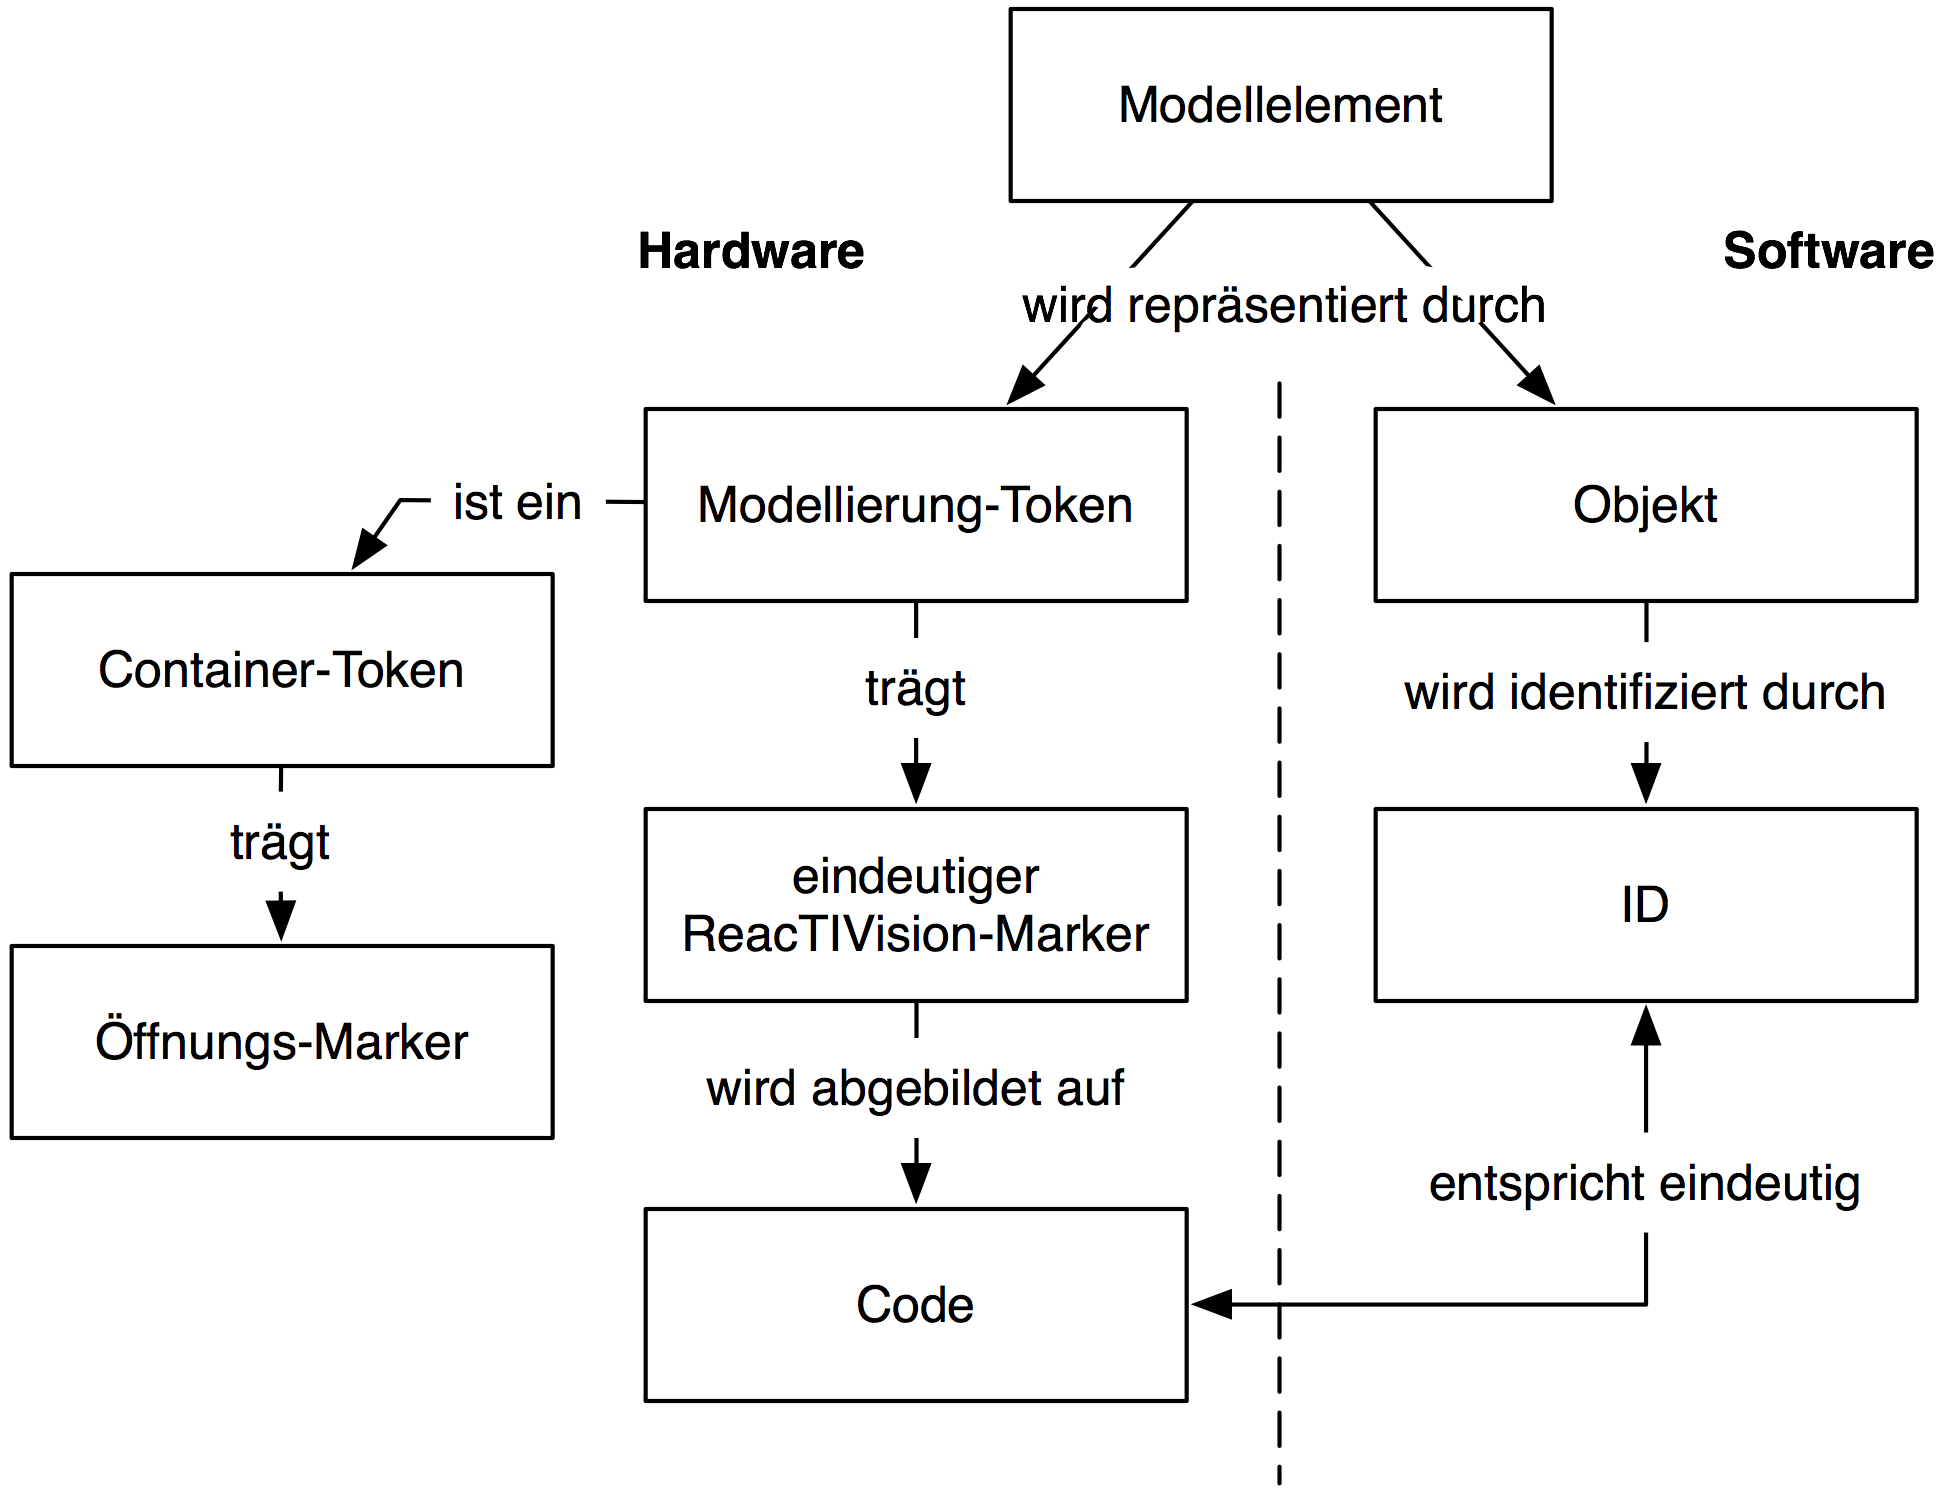
\includegraphics[height=3in]{img/ImplementierungInput/ElementTaxonomie.png}
	\caption{Modellelemente -- Taxonomie}
	\label{fig:img_ImplementierungInput_ElementTaxonomie}
\end{figure}

% subsubsection modellierungs_tokens (end)

\subsubsection{Einbettbare Tokens} % (fold)
\label{einbettbare_tokens}

Die einbettbaren Token erlauben wie in Kapitel XY beschrieben die Verschachtelung von Modellen und das Hinzufügen von Zusatzinformation. Sie werden in einem definierten Interaktionsvorgang an Information gebunden und dann in einen Container gelegt. Hinsichtlich des Hardware-Designs sind folgende Anforderungen zu beachten:
\begin{itemize}
	\item Die Token müssen klein genug sein, um auch mehrere Einheiten ein einem Container unterzubringen.
	\item Sie müssen gleichzeitig groß genug sein, um einen ReacTIVision-Code zur eindeutigen Identifikation anzubringen.
	\item Sie müssen so ausgeführt sein, dass haptisch oder akustisch erkennbar ist, ob in einem geschlossenen Container Tokens eingebettet sind oder nicht (z.B. durch Veränderung des Gewichts oder Geräusche beim Schütteln eines Containers).
\end{itemize}

Die einbettbaren Tokens wurden aus flexiblen Kunststoffmatten gefertigt und mit einem Metallstück versehen (siehe Abbildung \ref{fig:img_SystemNeu_EinbettbareTokens}), das einerseits als Griff dient und andererseits sowohl das Gewicht erhöht und akustisches Feedback beim Schütteln eines Container-Tokens verursacht. Die einbettbaren Tokens wurden exemplarisch in drei Ausführungen gefertigt, je nach Art und Anzahl der einzubettenden Information kann eine Definition weiterer Tokens sinnvoll sein. Folgende Tokens wurden für den aktuellen Entwicklungsstand des Werkzeugs angefertigt:
\begin{itemize}
	\item Einbettung von Teilmodellen (inhärente Kernfunktionalität des Werkzeugs)
	\item Einbettung von digitalen Ressourcen bzw. Dateien am lokalen Rechner (Erweiterung zur Verknüpfung des Modells mit den realen digitalen Ressourcen aus dem Arbeitskontext)
	\item Einbettung von Fotos (Erweiterung zur Verknüpfung des Modells mit dem realen Arbeitskontext, z.B. mittels Fotos von Arbeitsmitteln oder Personen)
\end{itemize}

\begin{figure}[htbp]
	\centering
		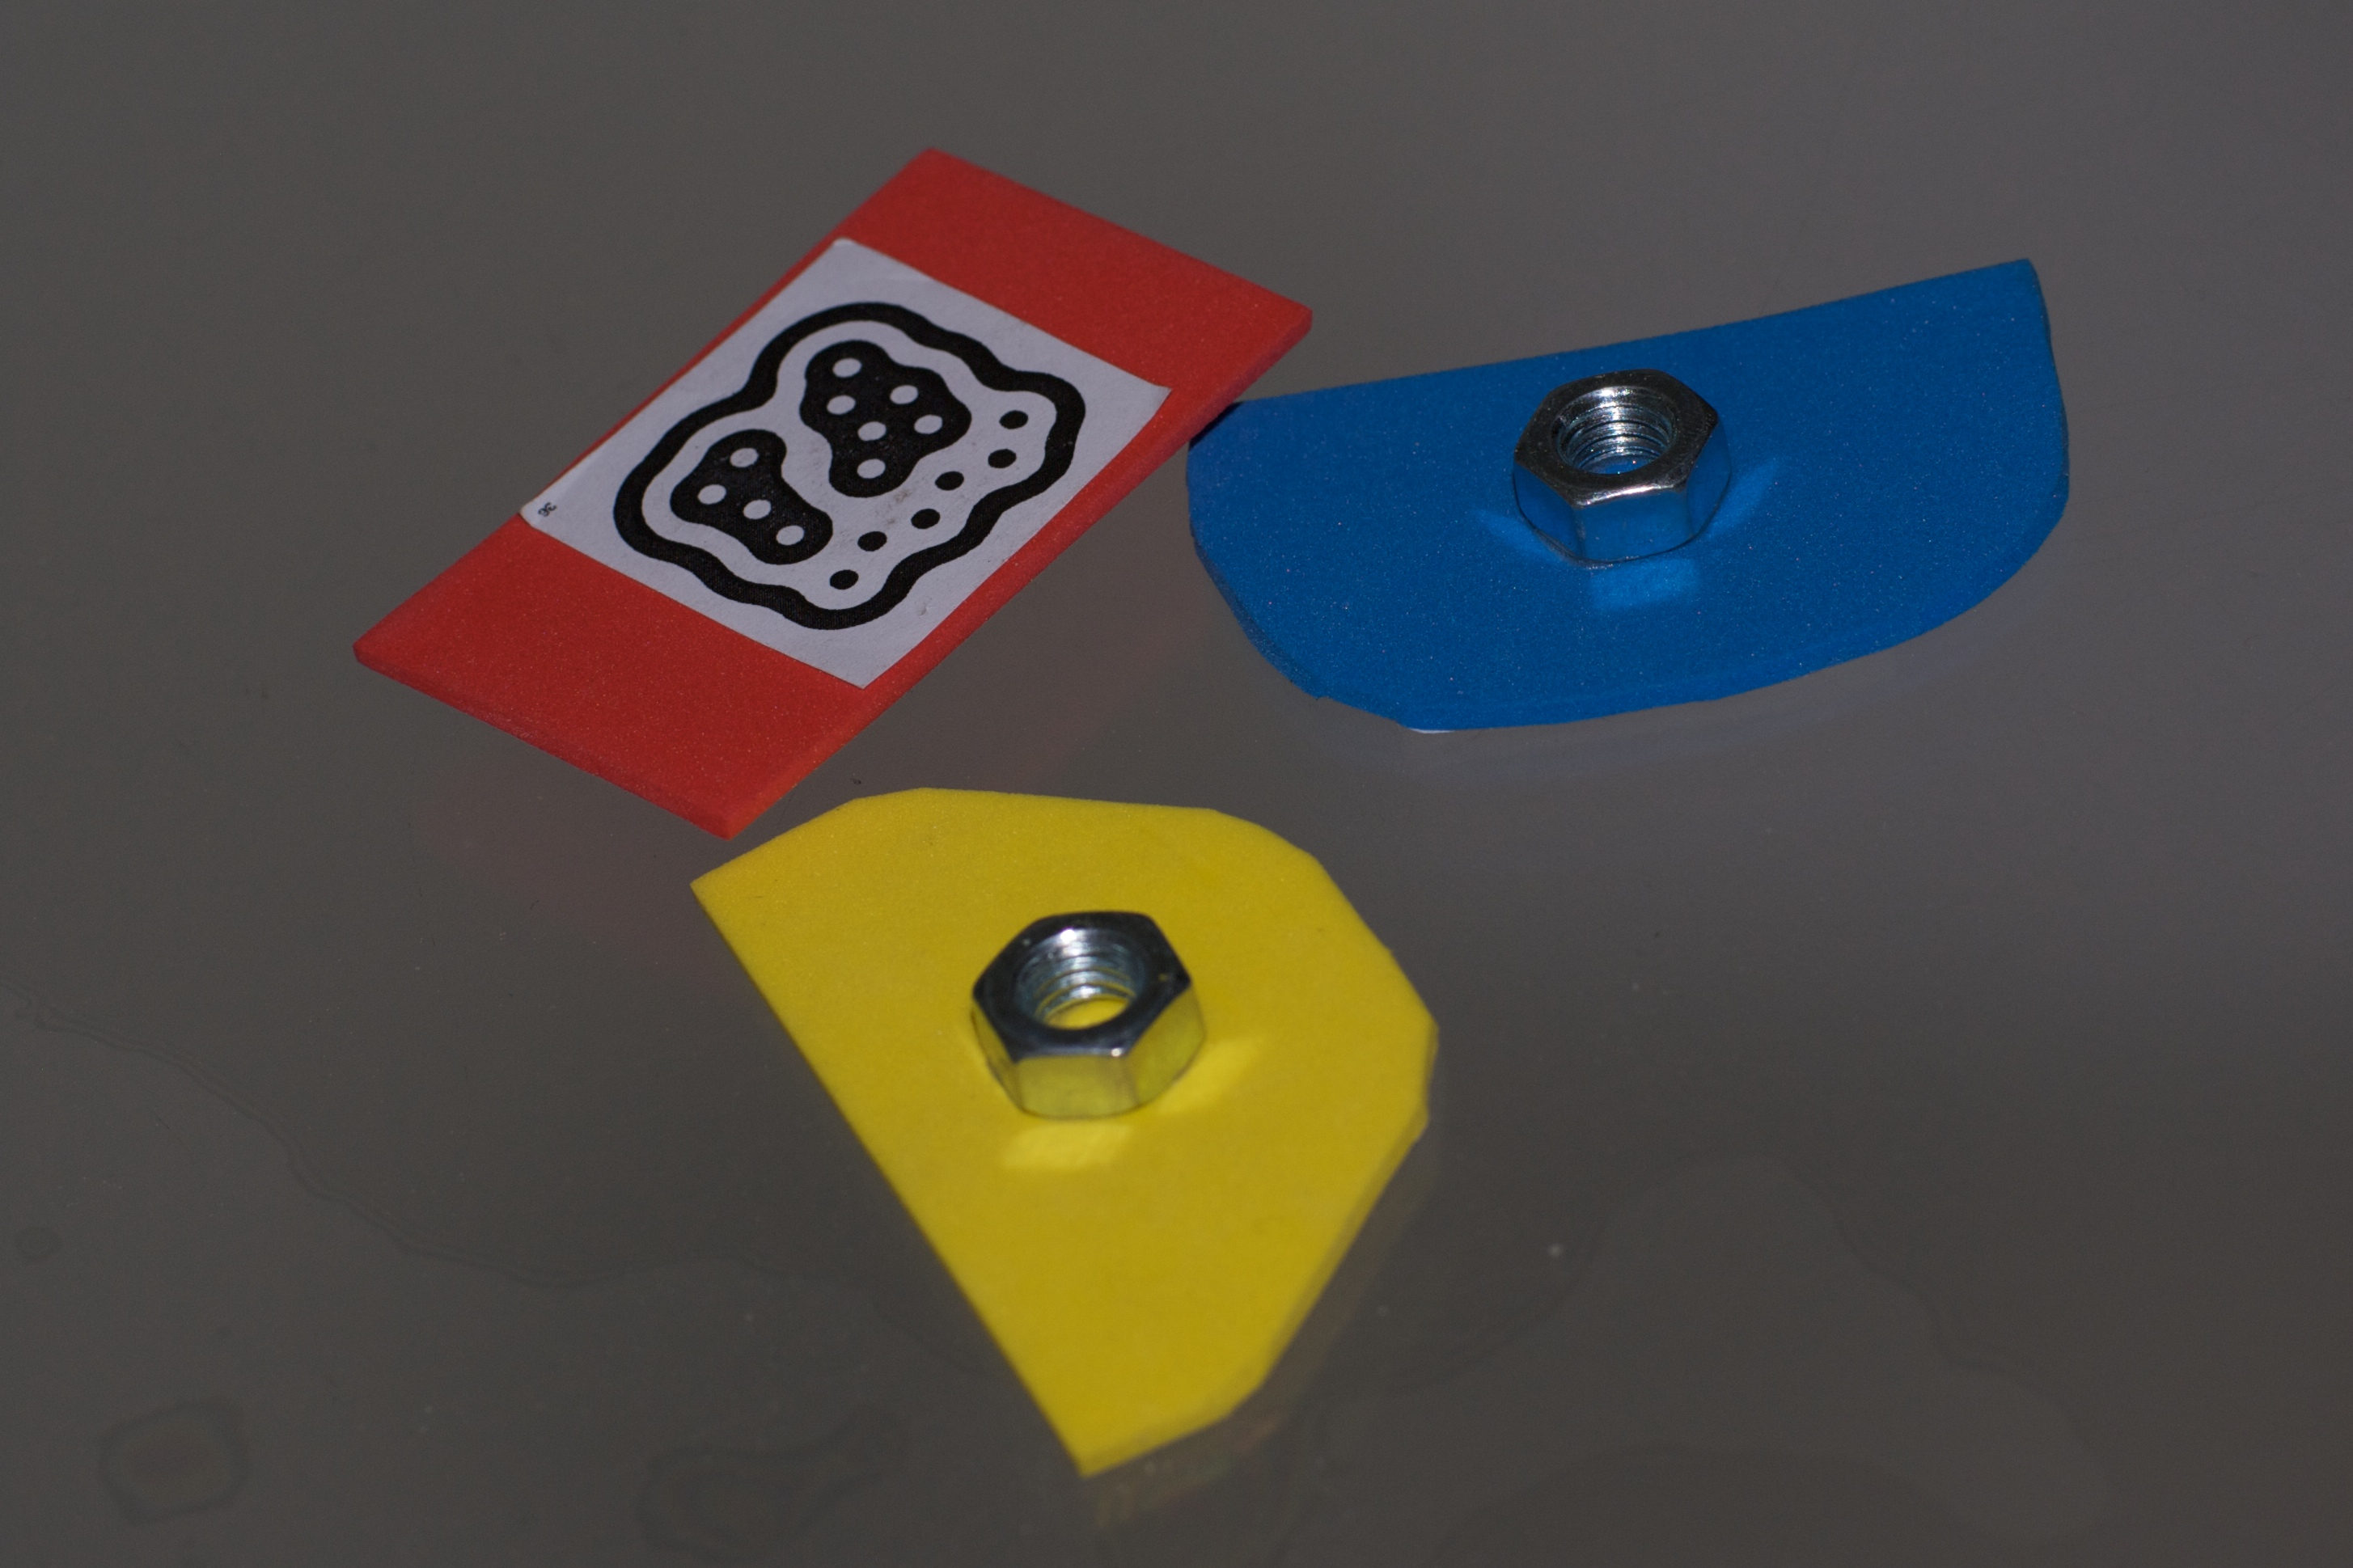
\includegraphics[height=2in]{img/SystemNeu/EinbettbareTokens.jpg}
	\caption{Einbettbare Tokens}
	\label{fig:img_SystemNeu_EinbettbareTokens}
\end{figure}

Alle Tokens sind auf der Unterseite mit einem ReacTIVision-Code versehen, der sie eindeutig identifiziert (siehe Abbildung \ref{fig:img_SystemNeu_EinbettbareTokens}). Aufgrund der beschränkten Größe der Tokens ist dieser Code von der Kamera, die die Tischoberfläche erfasst, nur in der Mitte der Oberfläche erfassbar (da dort die geringsten Linsen-Verzerrungen auftreten und der Code somit noch erkannt werden kann). Um etwaige Bedienungsprobleme zu vermeiden, wurde die deshalb die Interaktion mit einbettbaren Tokens (Registrierung, Binden von Information) auf die in Abbildung \ref{fig:img_ImplementierungInput_TischSeitenansicht} dargestellte zweite Kamera (“Registrierungs-Kamera“) verlegt, die durch die physische Nähe zu den Modellierenden die Codes der einbettbaren Tokens problemlos erfassen kann.

% subsubsection einbettbare_tokens (end)

\subsubsection{Werkzeug-Tokens} % (fold)
\label{ssub:werkzeug_tokens}

Neben den Tokens, die Modellierungsinhalte repräsentieren, wurden auch Tokens angefertigt, die der Interaktion mit dem System ansich und der Steuerung des Modellierungsablaufs dienen. Hier sind zwei Arten zu unterscheiden: einerseits gibt es Werkzeuge, die der Manipulation des Modells dienen (z.B. Herstellung von Verbindungen zwischen Tokens, Benennung von Tokens) und andererseits solche, die der Steuerung von modellierungsunterstützender Zusatzfunktionalität dienen (etwa Tokens, mit denen die Rückverfolgung der Modellierungshistorie gesteuert werden kann). Außerdem sind orthogonal zu dieser Klassifizierung noch Tokens zu unterscheiden, die beim Einsatz ein Ereignis auslösen und solche, die das System solange in einen anderen Zustand versetzen, bis sie wieder entfernt werden (gleich einem Taster). Im Folgenden werden die einzelnen Werkzeuge beschrieben und den eben definierten Kategorien zugeordnet.

\paragraph{Manipulation des Modells} % (fold)
\label{par:manipulation_des_modells}

Die bei der Verwendung des Systems wichtigsten Werkzeug-Tokens sind jene, die zur Benennung und Verbindung von Modellierungs-Tokens verwendet werden. Diese \emph{Markierungs-Tokens} sind als auf die Oberfläche aufsetzbare Stäbe konzipiert, die unten eine Standfläche aufweisen, welche auch den Code aufnimmt. Am oberen Ende ist eine Verbreiterung angebracht, die eine stabile Handhabung gewährleistet (siehe Abbildung \ref{fig:img_SystemNeu_Markierungstoken_alle}). Bedingt durch die kleine Standfläche kann nur der einfachste ReacTIVision-Code verwendet werden, der lediglich aus einem schwarzen Ring besteht. Das ReacTIVision-System erkennt diesen Ring nicht als regulären Code sondern als „Cursor“, also als Zeiger, der ausschließlich eine Position in der Ebene besitzt, aber keine Rotation aufweist. Für die Verwendung zur Markierung von Modellierungs-Tokens zum Zwecke der Benennung oder Verbindung ist dies auch nicht notwendig.

\begin{figure}[htbp]
	\centering
		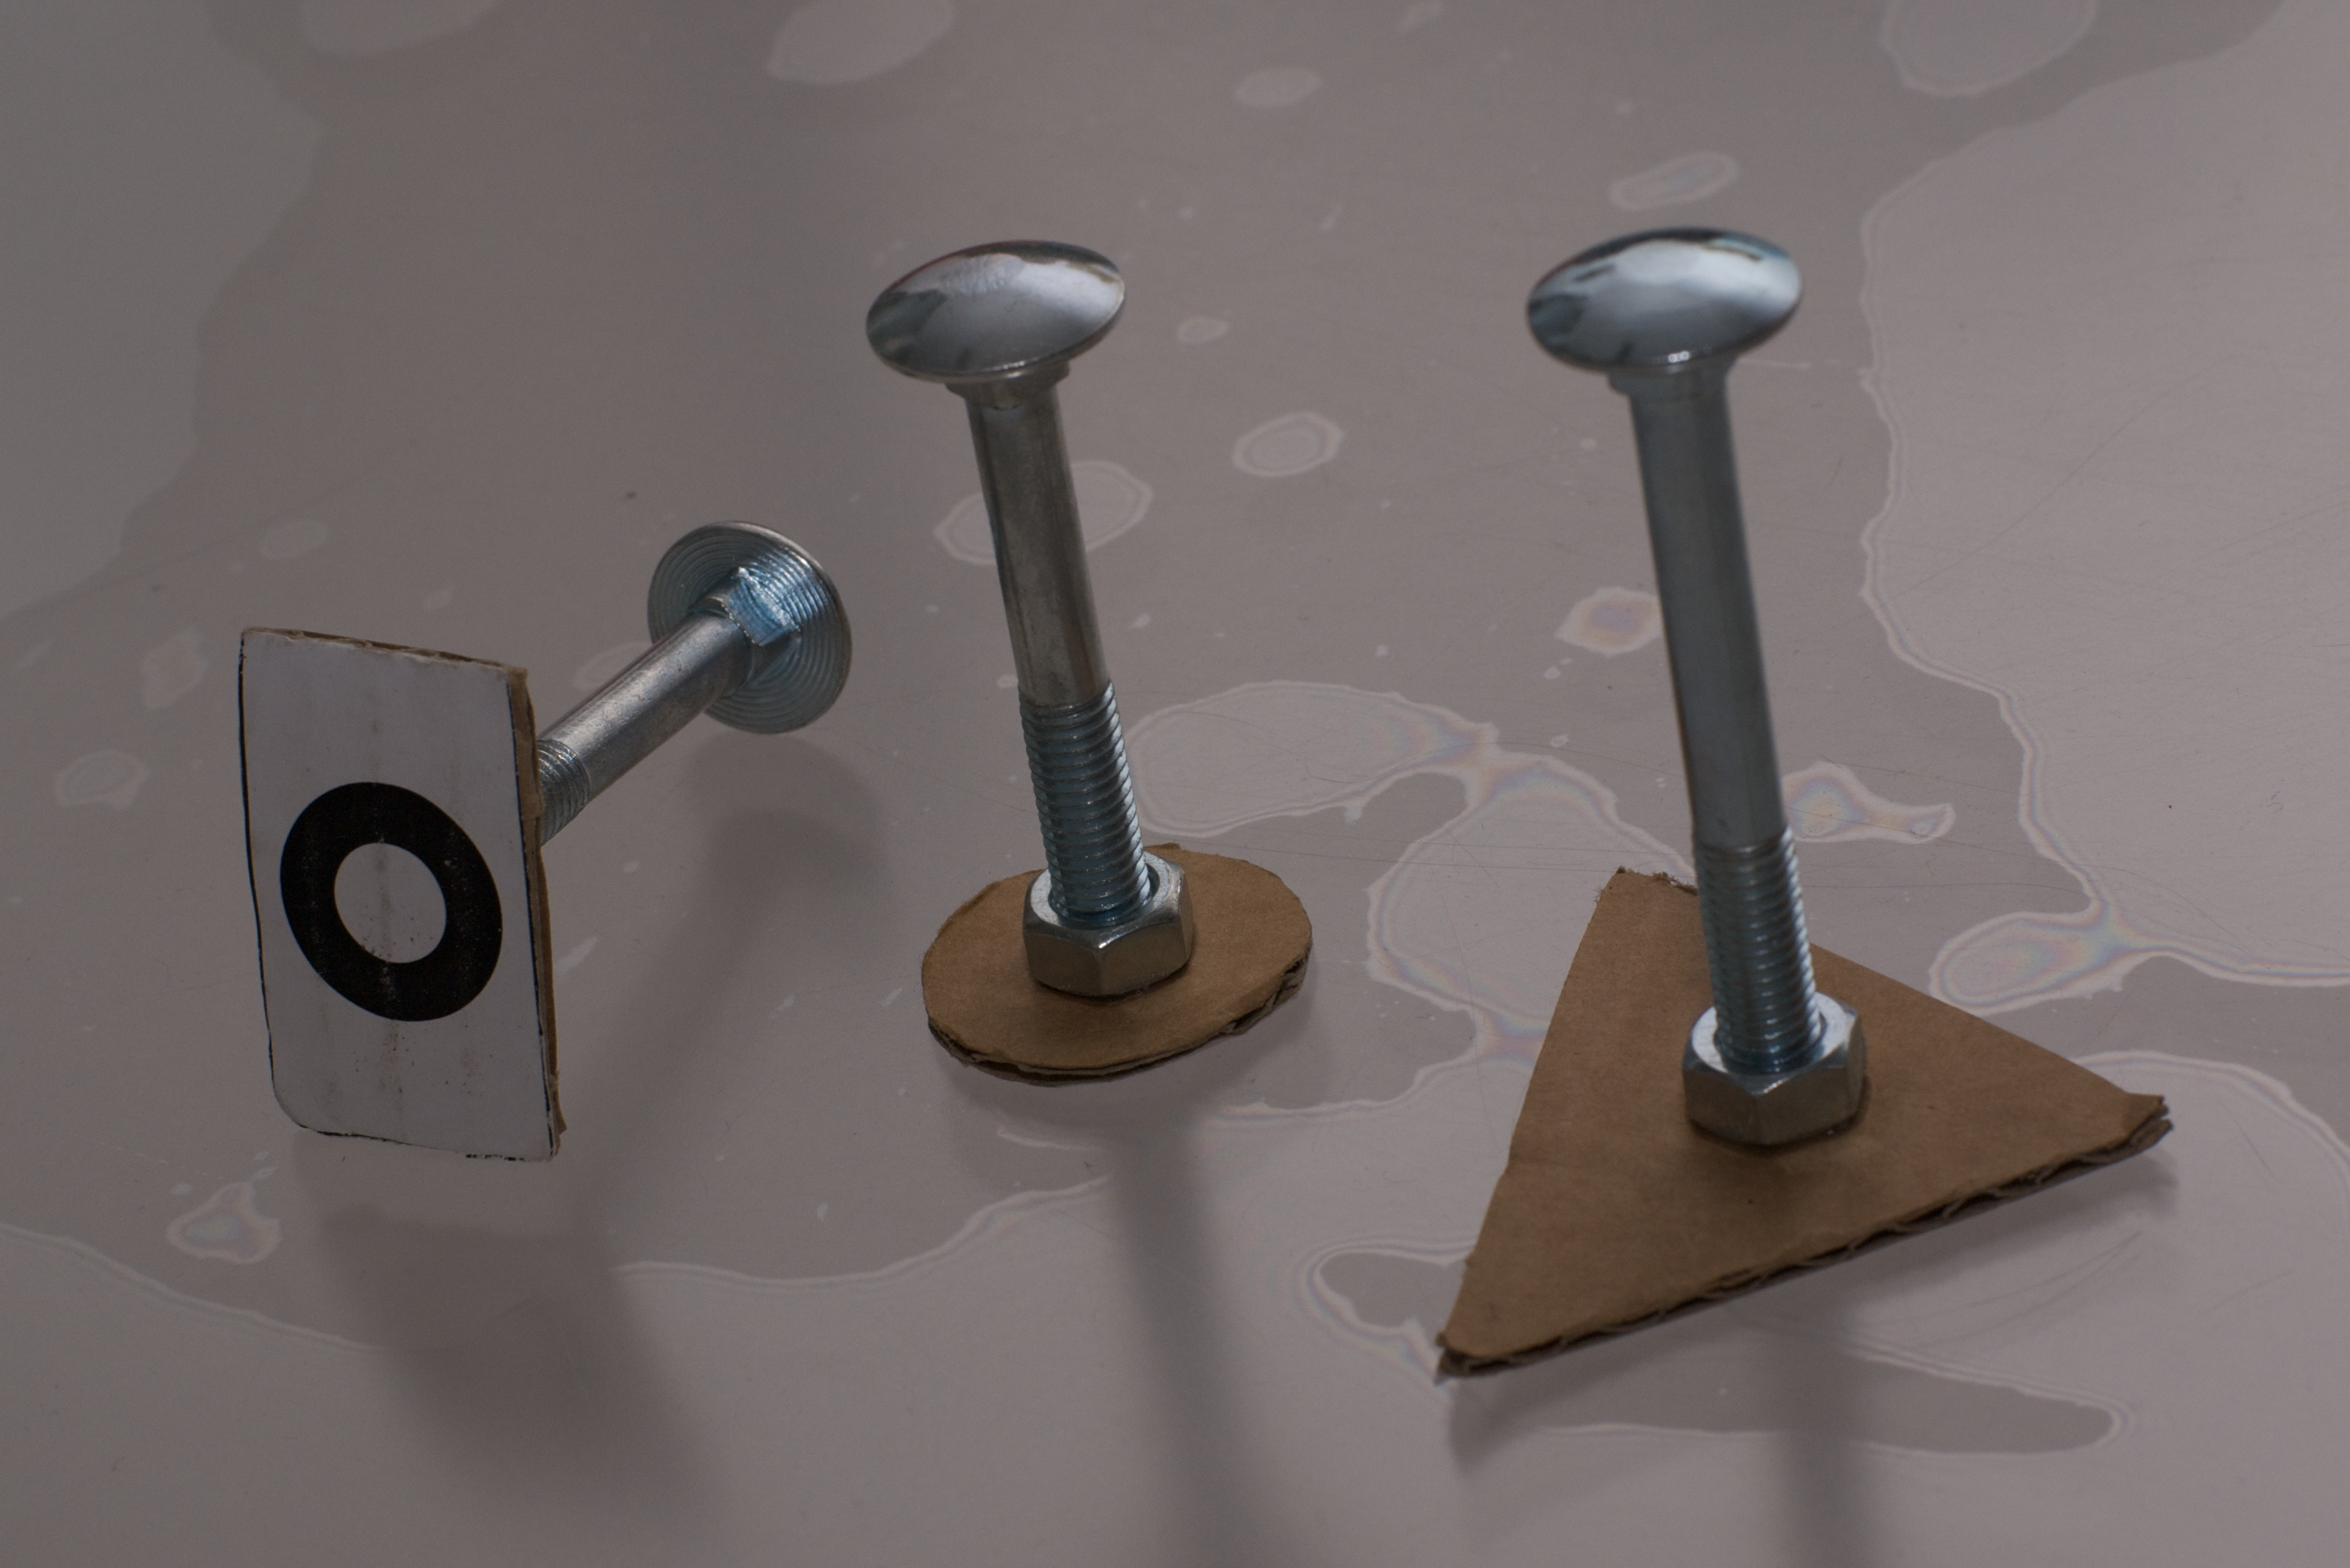
\includegraphics[height=2in]{img/SystemNeu/Markierungstoken_alle.jpg}
	\caption{Markierung-Token}
	\label{fig:img_SystemNeu_Markierungstoken_alle}
\end{figure}


Das Modellierungswerkzeug muss zwischen unterschiedlichen Arten von Verbindungen unterscheiden können, da diese bei der vorgestellten Art der Externalisierung zum Einsatz kommen können. Im Wesentlichen ist zwischen ungerichteten und gerichteten Verbindern zu unterscheiden. Im Gegensatz zu ungerichteten Verbindern weisen gerichtete Verbinder Pfeilspitzen an einem Ende oder an beiden Enden auf. Für die Werkzeug-Tokens bedeutet dies, dass neben den bereits beschriebenen, einfachen Markierungs-Tokens auch solche zum Einsatz kommen, die anstatt einer runden Grundfläche eine größere, dreieckige Grundfläche aufweisen, die eine Pfeilspitze symbolisiert (siehe Abbildung \ref{fig:img_SystemNeu_Markierungstoken_alle}). Technisch werden die beiden Arten von Markierungs-Tokens durch einen zweiten Cursor-Code unterschieden, der an Tokens mit dreieckiger Grundfläche zusätzlich angebracht ist.

Die Markierungs-Tokens sind der Kategorie der ein Ereignis auslösenden Tokens zuzuordnen. Dies bedeutet, dass das System zu jenem Zeitpunkt eine Aktion setzt, an dem das Token auf die Oberfläche aufgesetzt wird. Wird ein Markierungs-Token auf der Oberfläche belassen, verursacht es keine weiteren Aktionen bis es entfernt und erneut aufgesetzt wird.

Dem hingegen ist das nächste hier behandelte Token der Kategorie der den Systemzustand beeinflussenden Tokens zuzuordnen. Es hat also solange Auswirkungen auf den Modellierungsablauf, solange es auf der Oberfläche belassen wird. Die konkrete Funktion dieses Tokens ist der Wechsel in einen Werkzeugmodus, der ein explizites Entfernen bzw. Löschen von Bestandteilen des Modells, insbesondere Verbindungen, erlaubt. Das Token ist als Radiergummi ausgeführt und codiert so die Metapher des expliziten Löschens von Information aus dem Modell (siehe Abbildung \ref{fig:img_SystemNeu_Loeschtoken}). An der Unterseite des Tokens ist eine ReacTIVision-Code angebracht um es gegenüber dem System eindeutig zu identifizieren.

\begin{figure}[htbp]
	\centering
		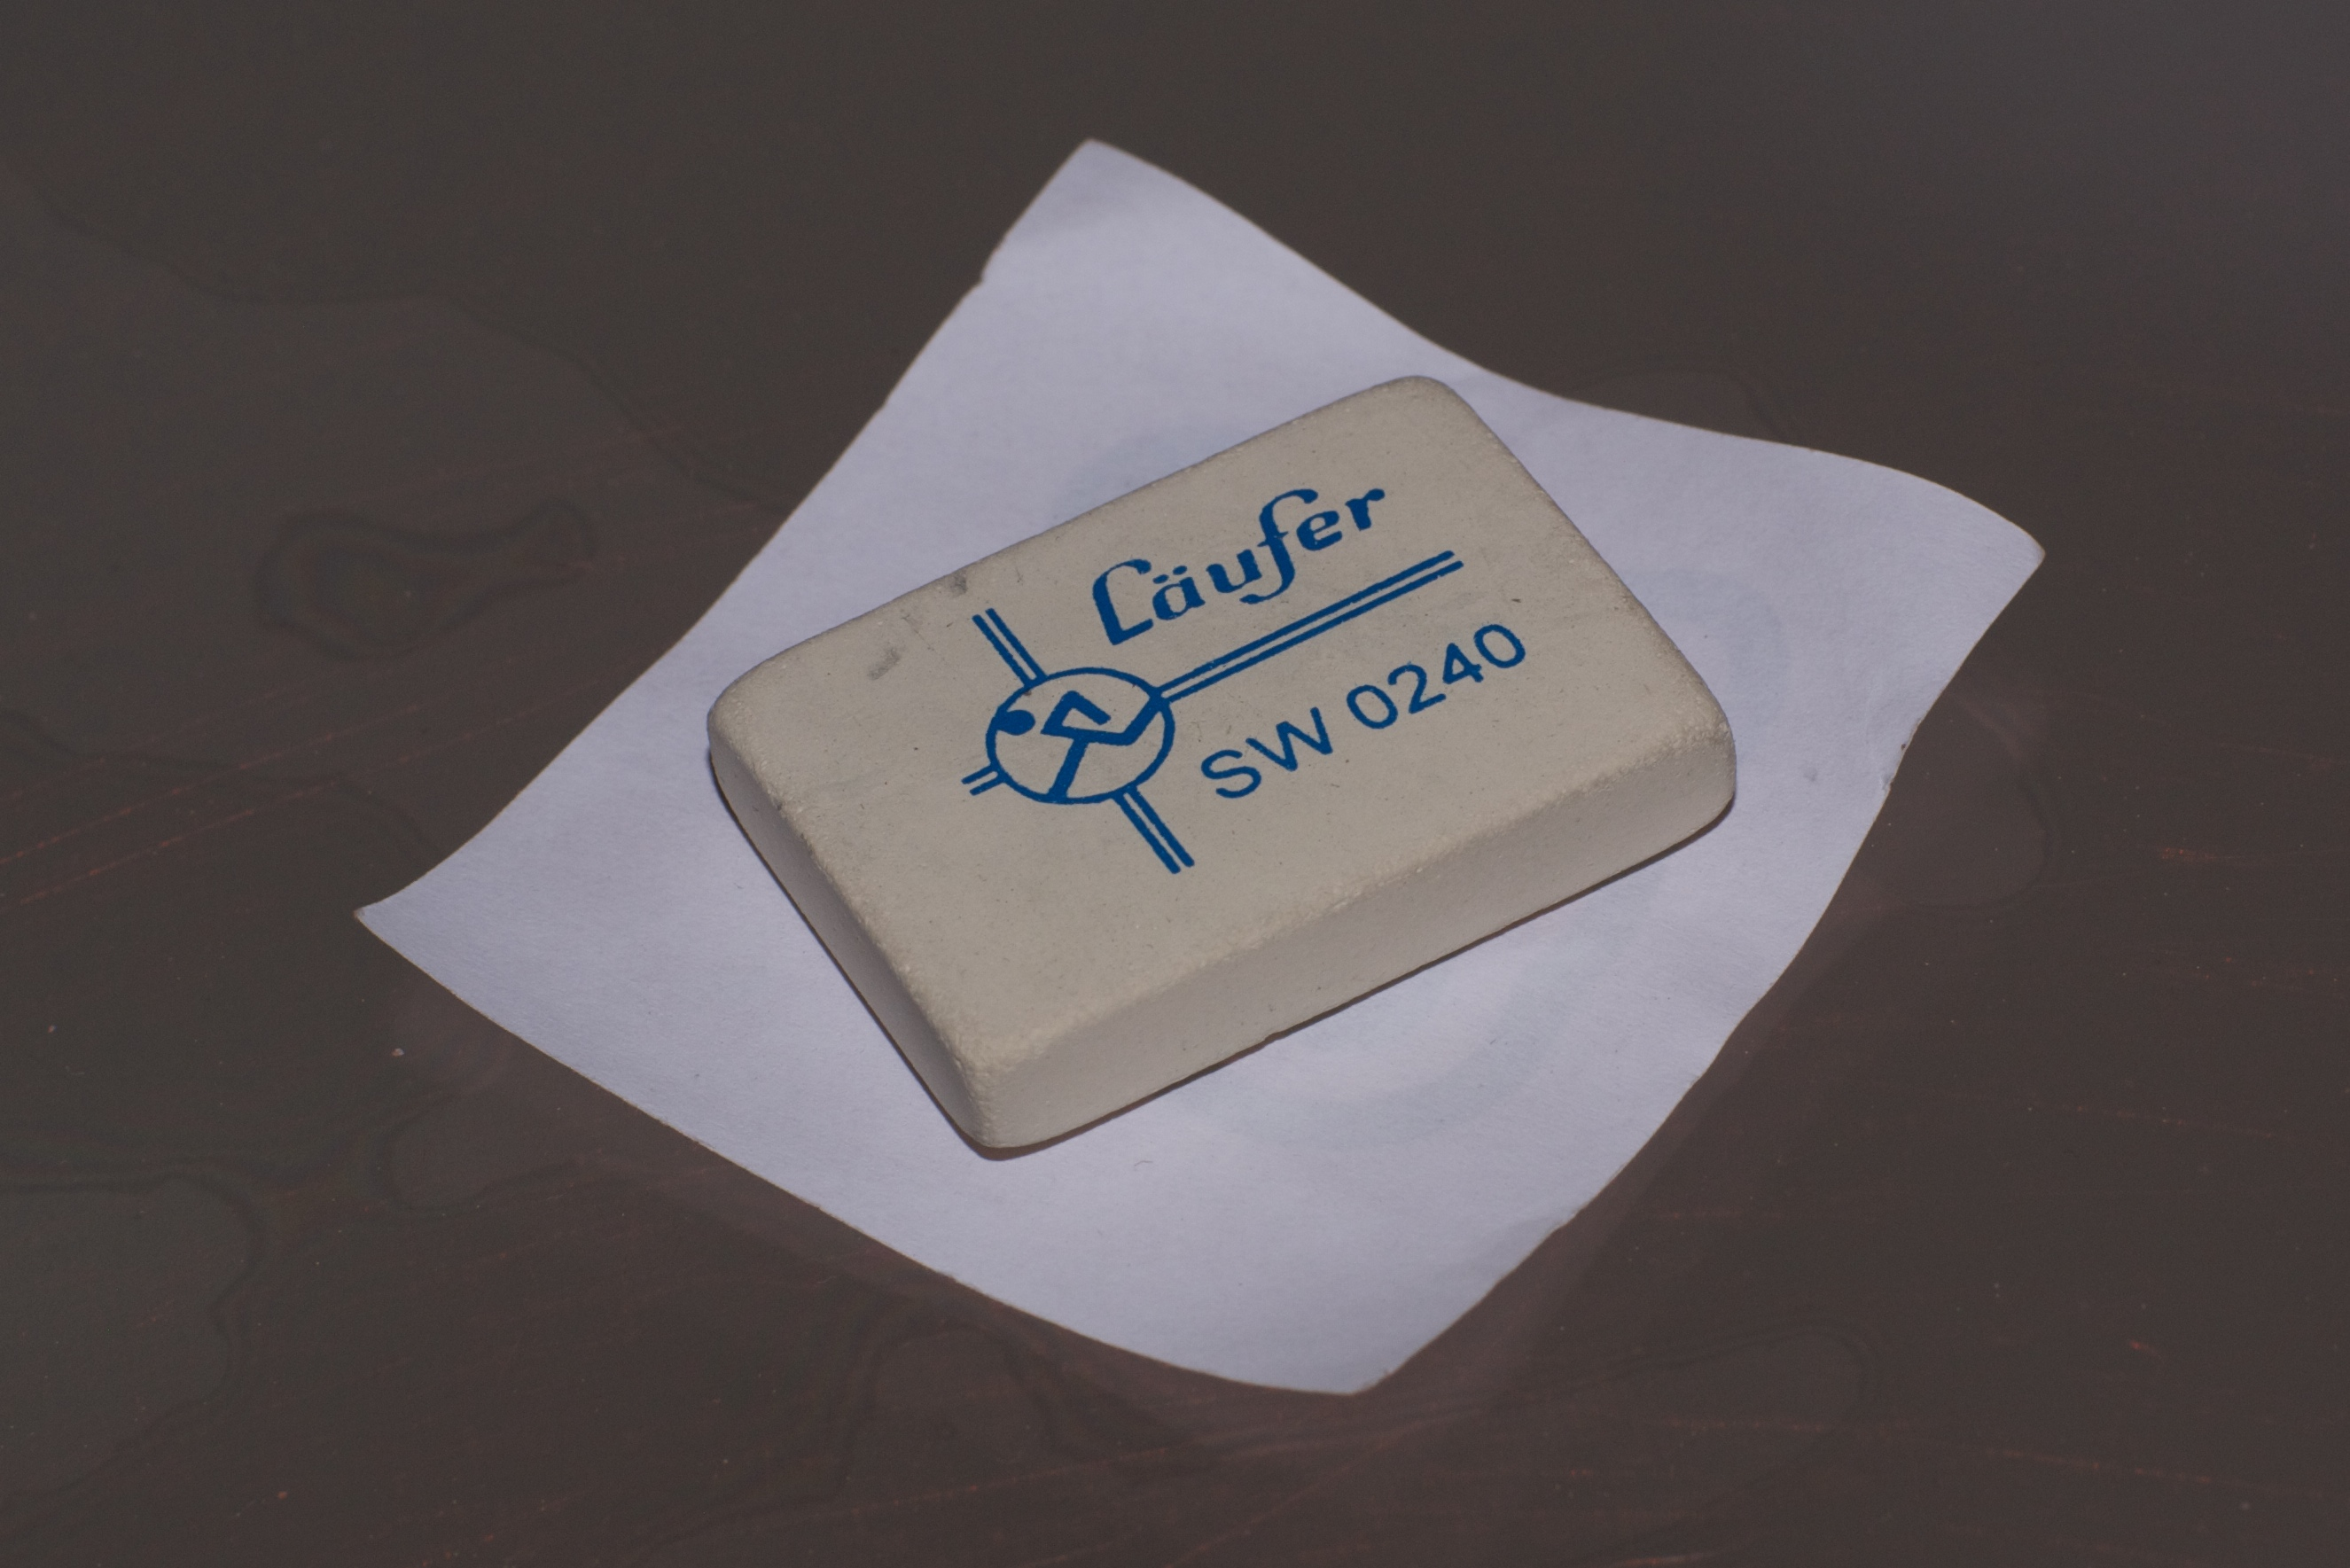
\includegraphics[height=2in]{img/SystemNeu/Loeschtoken.jpg}
	\caption{Lösch-Token}
	\label{fig:img_SystemNeu_Loeschtoken}
\end{figure}


Der Einsatz der \emph{Lösch-Tokens} verändert im System im Wesentlichen die Interpretation des Markierungs-Tokens, das nun anstatt der Herstellung einer Verbindung das Löschen derselben auslöst. Der  zugehörige Interaktionsablauf ist im Detail in Abschnitt \ref{sub:löschen_von_elementen} dargelegt.

Ein weiteres Werkzeug im Kontext der Manipulation des Modells ist das \emph{Registrierungs-Token} für die Benennung von Blöcken mittels handgeschriebenen Haftnotizen. Wie in Abschnitt \ref{sub:benennen_von_modellelementen} im Detail ausgeführt, gibt es zwei Möglichkeiten um ein Modellierungs-Token zu benennen. Einerseits kann der herkömmlich Eingabeweg über die Tastatur gewählt werden, andererseits ist es möglich, die Modellierungs-Tokens mittels aufgeklebten Haftnotizen zu benennen. Um die handgeschriebene Information in die digitale Information übernehmen zu können, wird diese mittels Bildanalyse-Verfahren aus einem Bild extrahiert, das von der oben bereits erwähnten Registrierungskamera (siehe Abbildung \ref{fig:img_ImplementierungInput_TischSeitenansicht}) aufgenommen wird. Die Aufnahme wird durch das erwähnte Registrierungstoken ausgelöst. Dieses fungiert gleichzeitig als Halter für noch unbeschriftete Haftnotizen und weist am linken und rechten Rand jeweils einen ReacTIVision-Code auf (siehe Abbildung \ref{fig:img_SystemNeu_Benennungstoken}). Diese beiden Codes erlauben es, im Bild die Position der Haftnotiz und damit die zu extrahierende Information zu identifizieren. 

\begin{figure}[htbp]
	\centering
		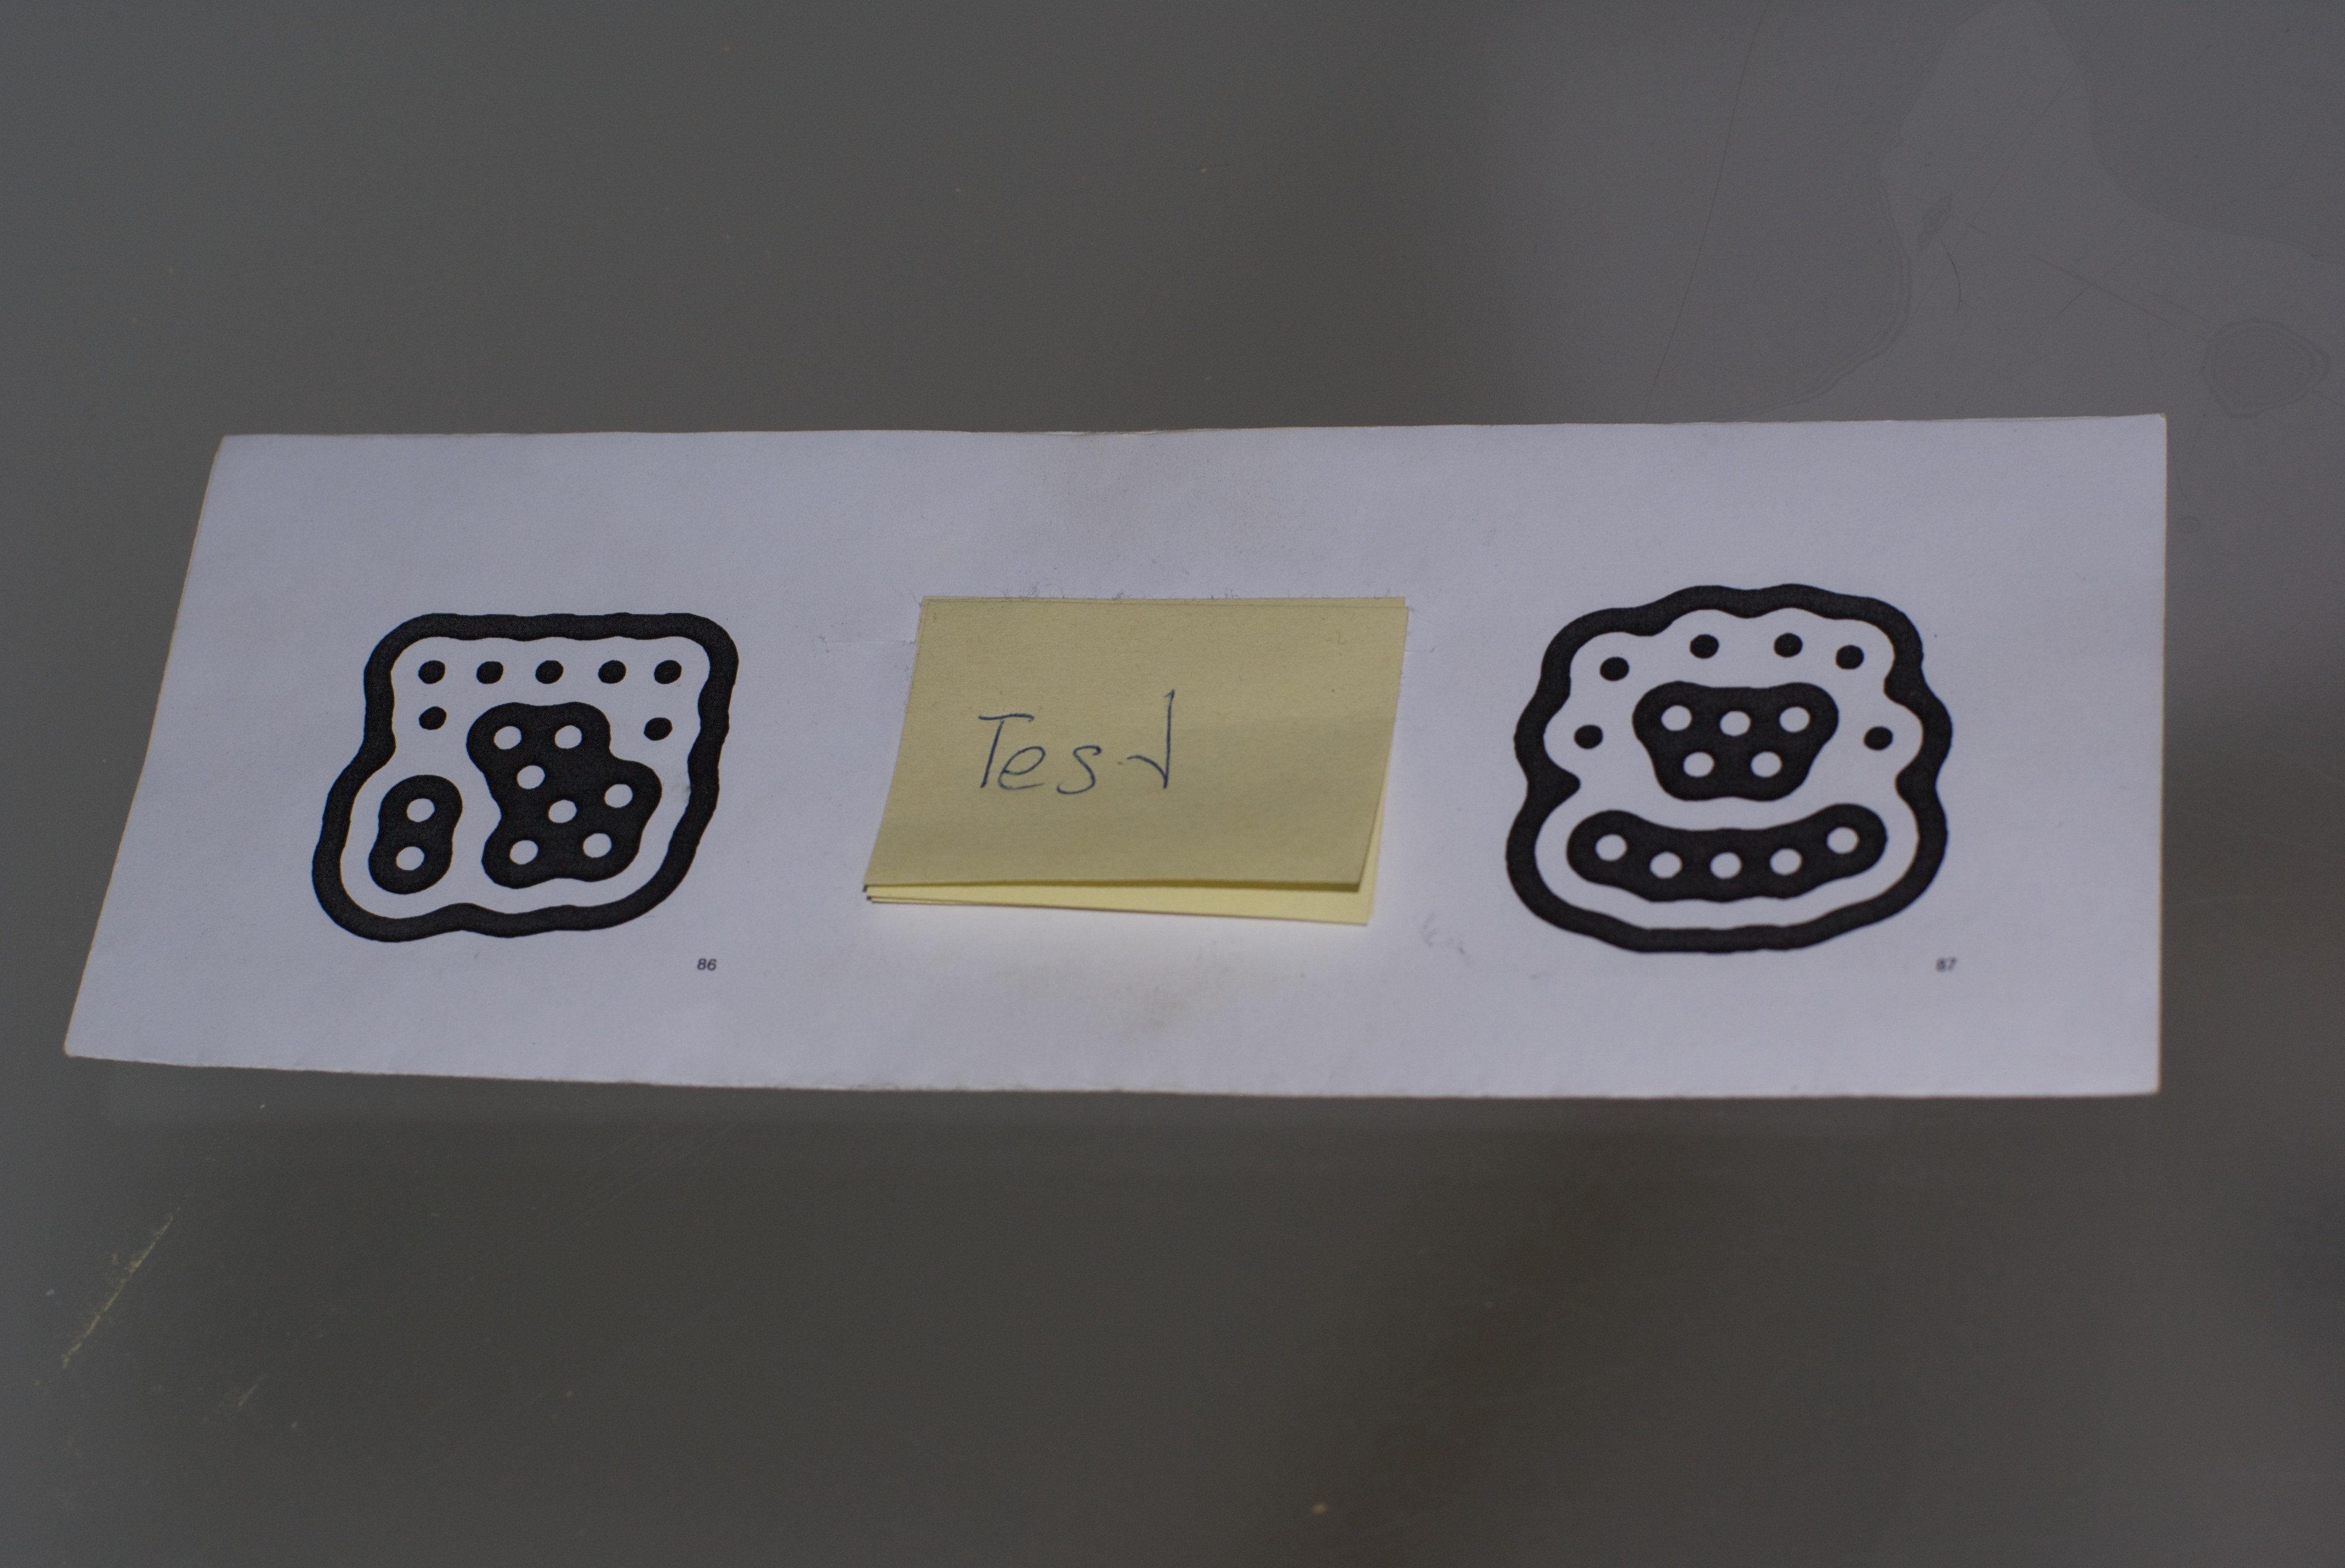
\includegraphics[height=2in]{img/SystemNeu/Benennungstoken.jpg}
	\caption{Registrierungstoken}
	\label{fig:img_SystemNeu_Benennungstoken}
\end{figure}

Das Registrierungstoken ist in die Kategorie der Ereignis auslösenden Tokens einzuordnen. Seine Verwendung erwies sich im praktischen Einsatz als wenig intuitiv und technisch instabil bzw. zu langsam, so dass -- wie erwähnt -- als alternativer Eingabeweg zusätzlich eine Tastatur ins System aufgenommen wurde. Die Interaktionsabläufe sind in beiden Fällen ähnlich und werden im Detail in Abschnitt \ref{sub:benennen_von_modellelementen} dargestellt.
% paragraph manipulation_des_modells (end)

\paragraph{Steuerung von Unterstützungsfunktionen} % (fold)
\label{par:steuerung_von_unterstützungsfunktionen}

Im Werkzeug wurden entsprechend den Anforderungen aus Kapitel XY den Modellierungsablauf unterstützende Funktionen implementiert. Diese werden über dezidierte Werkzeug-Tokens gesteuert. Der Anwendungsbereich dieser Art von Tokens ist die Steuerung aller Funktionen, die im Kontext der Verfolgbarkeit der Modellierungs-Historie umgesetzt wurden. 

Das \emph{Snapshot-Token} dient der durch die Benutzer ausgelösten Speicherung des aktuellen Systemzustandes. Wie in Kapitel XY beschrieben, verfolgt das System den Modellierungsablauf und speichert selbsttätig stabile Systemzustände (zur Identifikation dieser Zustände siehe Abschnitt \ref{sec:benutzerinteraktion_mit_dem_werkzeug}). Zusätzlich können Benutzer mit eben dem hier beschriebenen Token die explizite Aufnahme des aktuellen Modellzustandes veranlassen, wenn ihnen dieser wesentlich erscheint. Das Token ist als ereignis-auslösendes Element konzipiert und wird durch kurzes Aufsetzen des Tokens auf die Modellierungsoberfläche aktiviert. Physisch ist es prototypisch als großes rotes Quadrat ausgeführt, an dessen Oberseite ein Griffstück angebracht ist (siehe Abbildung \ref{fig:img_SystemNeu_Snapshottoken}). Auf der Unterseite sitzt wiederum ein ReacTIVision-Code zur Identifikation des Tokens.

\begin{figure}[htbp]
	\centering
		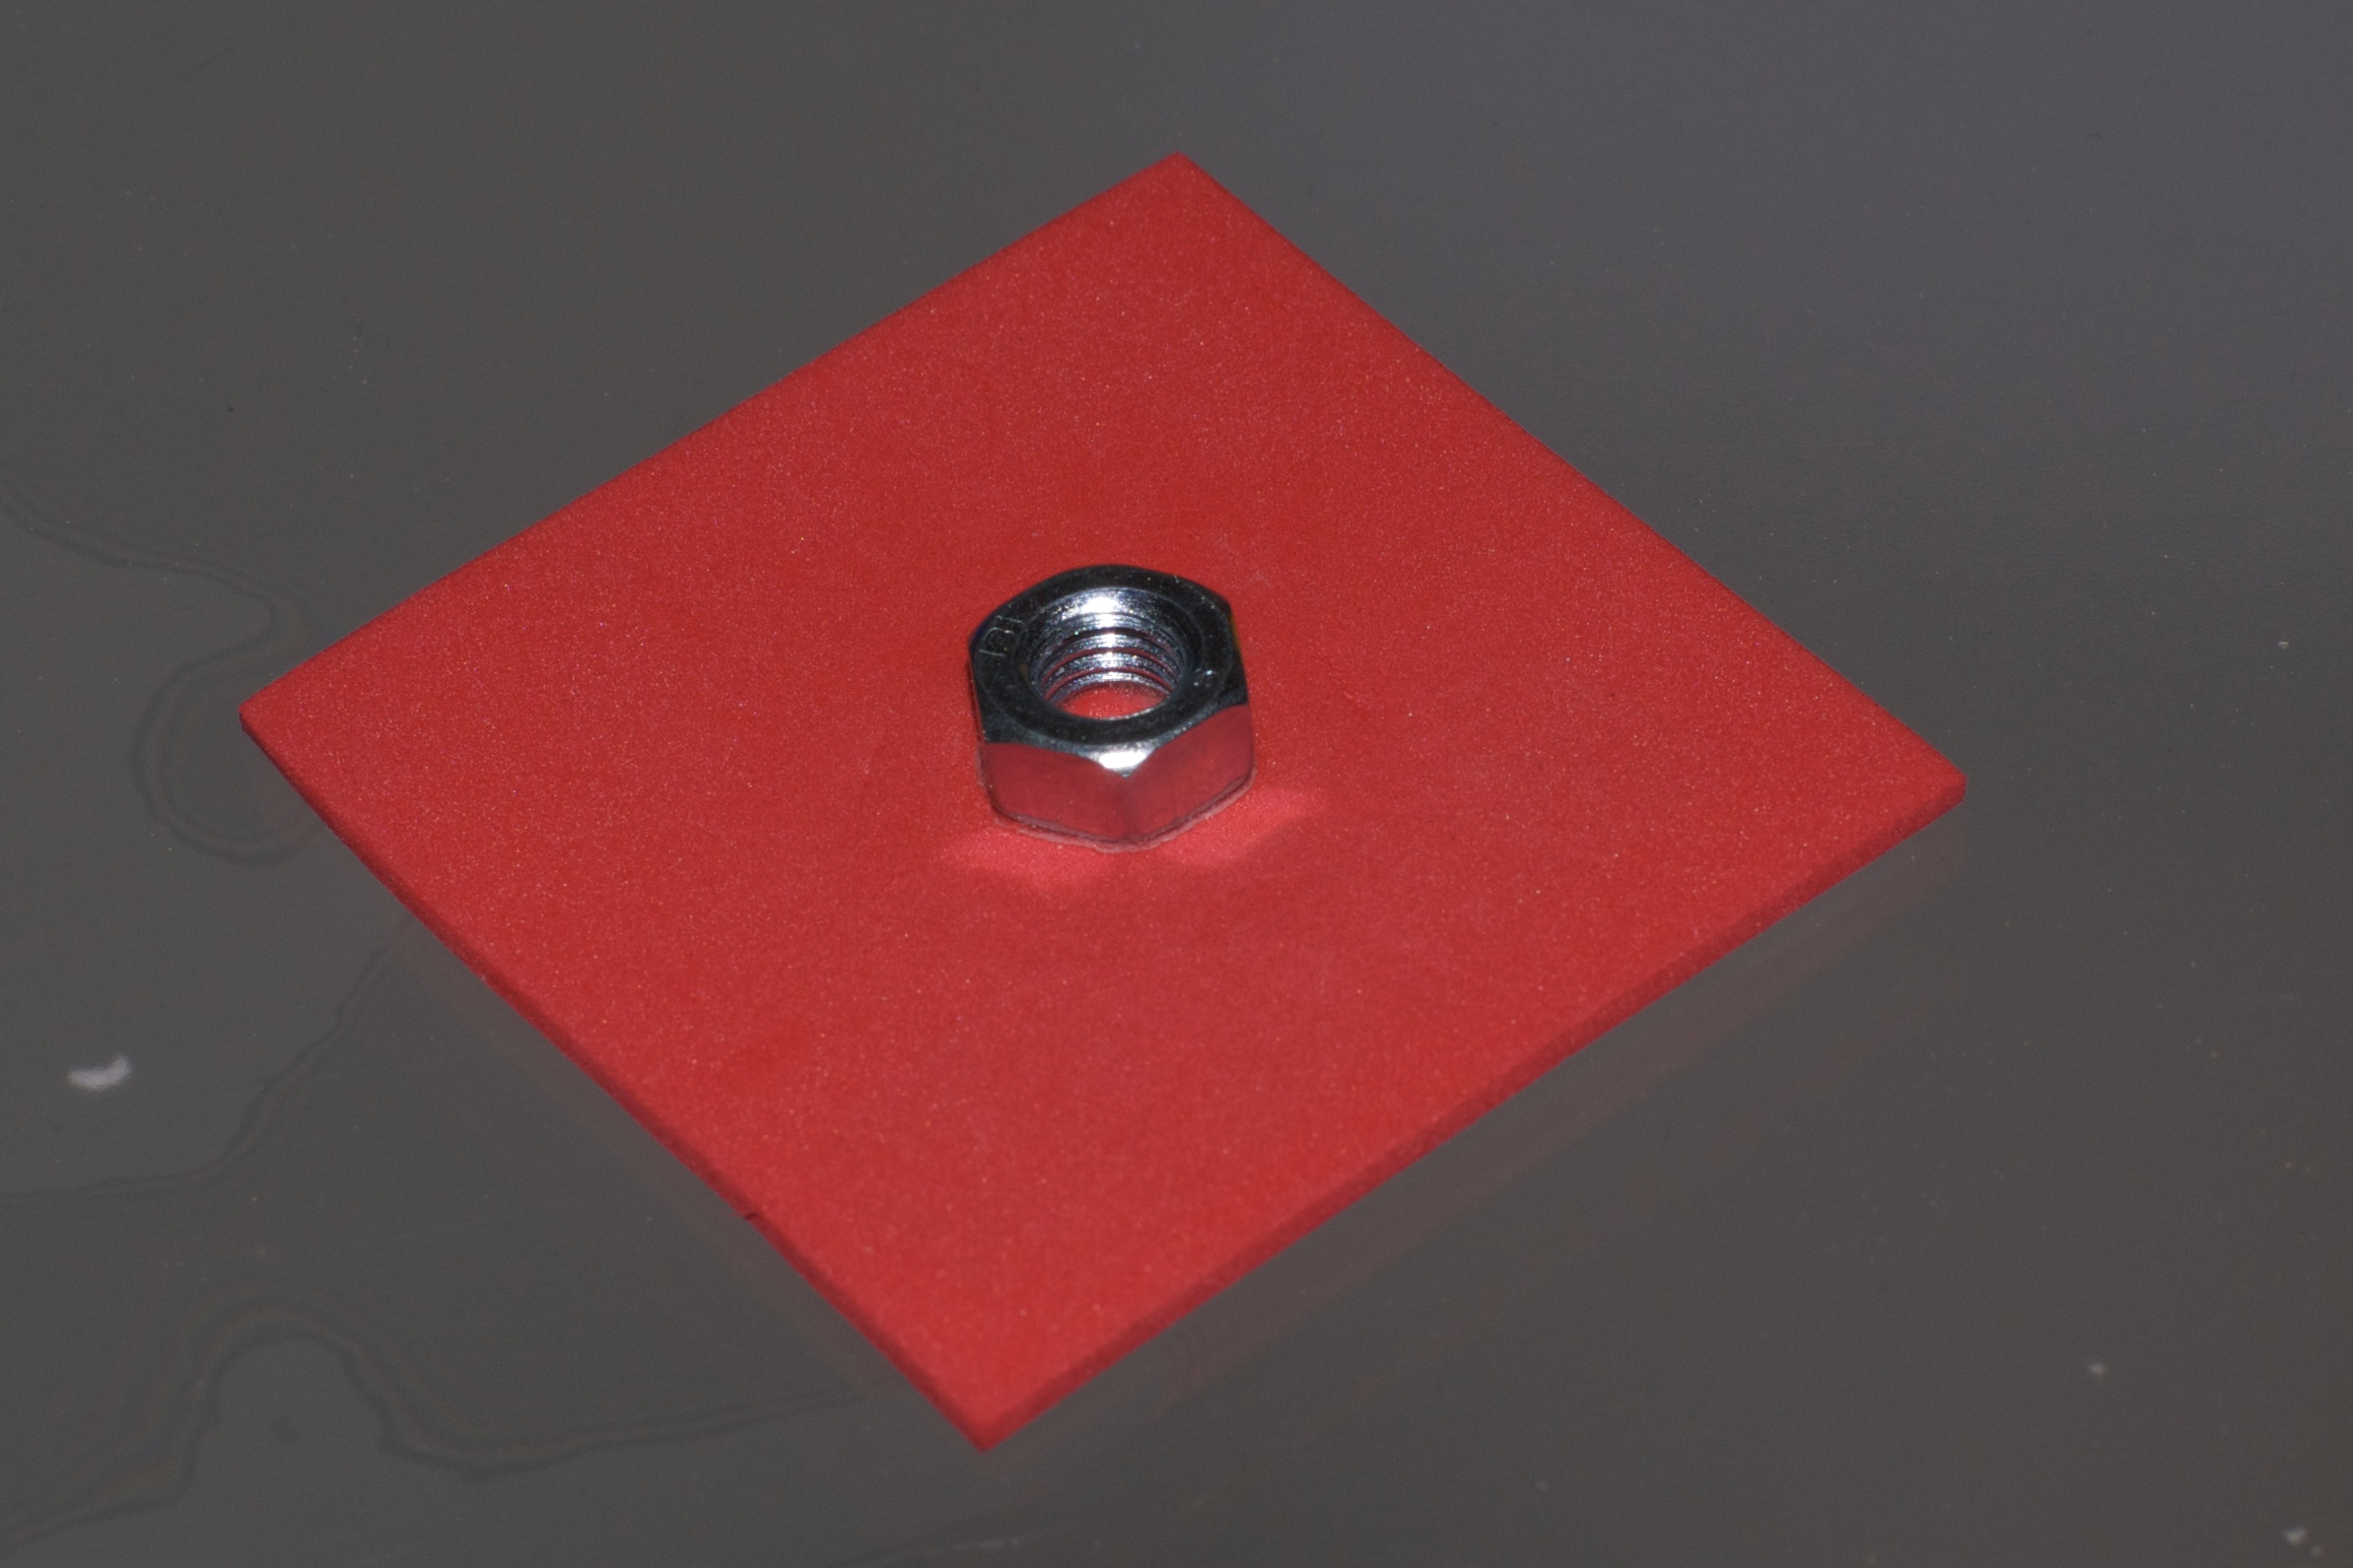
\includegraphics[height=2in]{img/SystemNeu/Snapshottoken.jpg}
	\caption{Snapshot-Token}
	\label{fig:img_SystemNeu_Snapshottoken}
\end{figure}

Neben der Speicherung von Modellzuständen können diese auch wieder abgerufen und in ihrer zeitlichen Sequenz dargestellt werden. Zur Aktivierung des Historien-Modus und zur Navigation in der Zeitlinie wurde ein weiteres Token eingeführt, das als einziges sowohl der zustandsverändernden als auch der ereignisauslösenden Token-Kategorie zuzuordnen ist. Zustandsverändernd wirkt das \emph{History-Token} insofern, als dass das Aufsetzen auf die Oberfläche das System in den Historienmodus schaltet und ein Entfernen die aktuelle Modell-Ansicht wieder herstellt. Durch Rotation des Token im bzw. gegen den Uhrzeigersinn kann nun durch die in ihrer zeitlichen Abfolge angeordneten gespeicherten Modellzustände navigiert werden. Die Rotation löst dabei jeweils nach einem bestimmten zurückgelegten Drehwinkel ein Ereignis aus, das den entsprechend vorhergehenden bzw. nachfolgenden Systemzustand abruft. Um die Rotation möglichst natürlich handhabbar zu machen, ist das Token mit runder Grundfläche etwa handflächengroß ausgeführt (siehe Abbildung \ref{fig:img_SystemNeu_Historytoken}). Auf der Unterseite der Grundfläche ist wiederum der ReacTIVision-Code angebracht.

\begin{figure}[htbp]
	\centering
		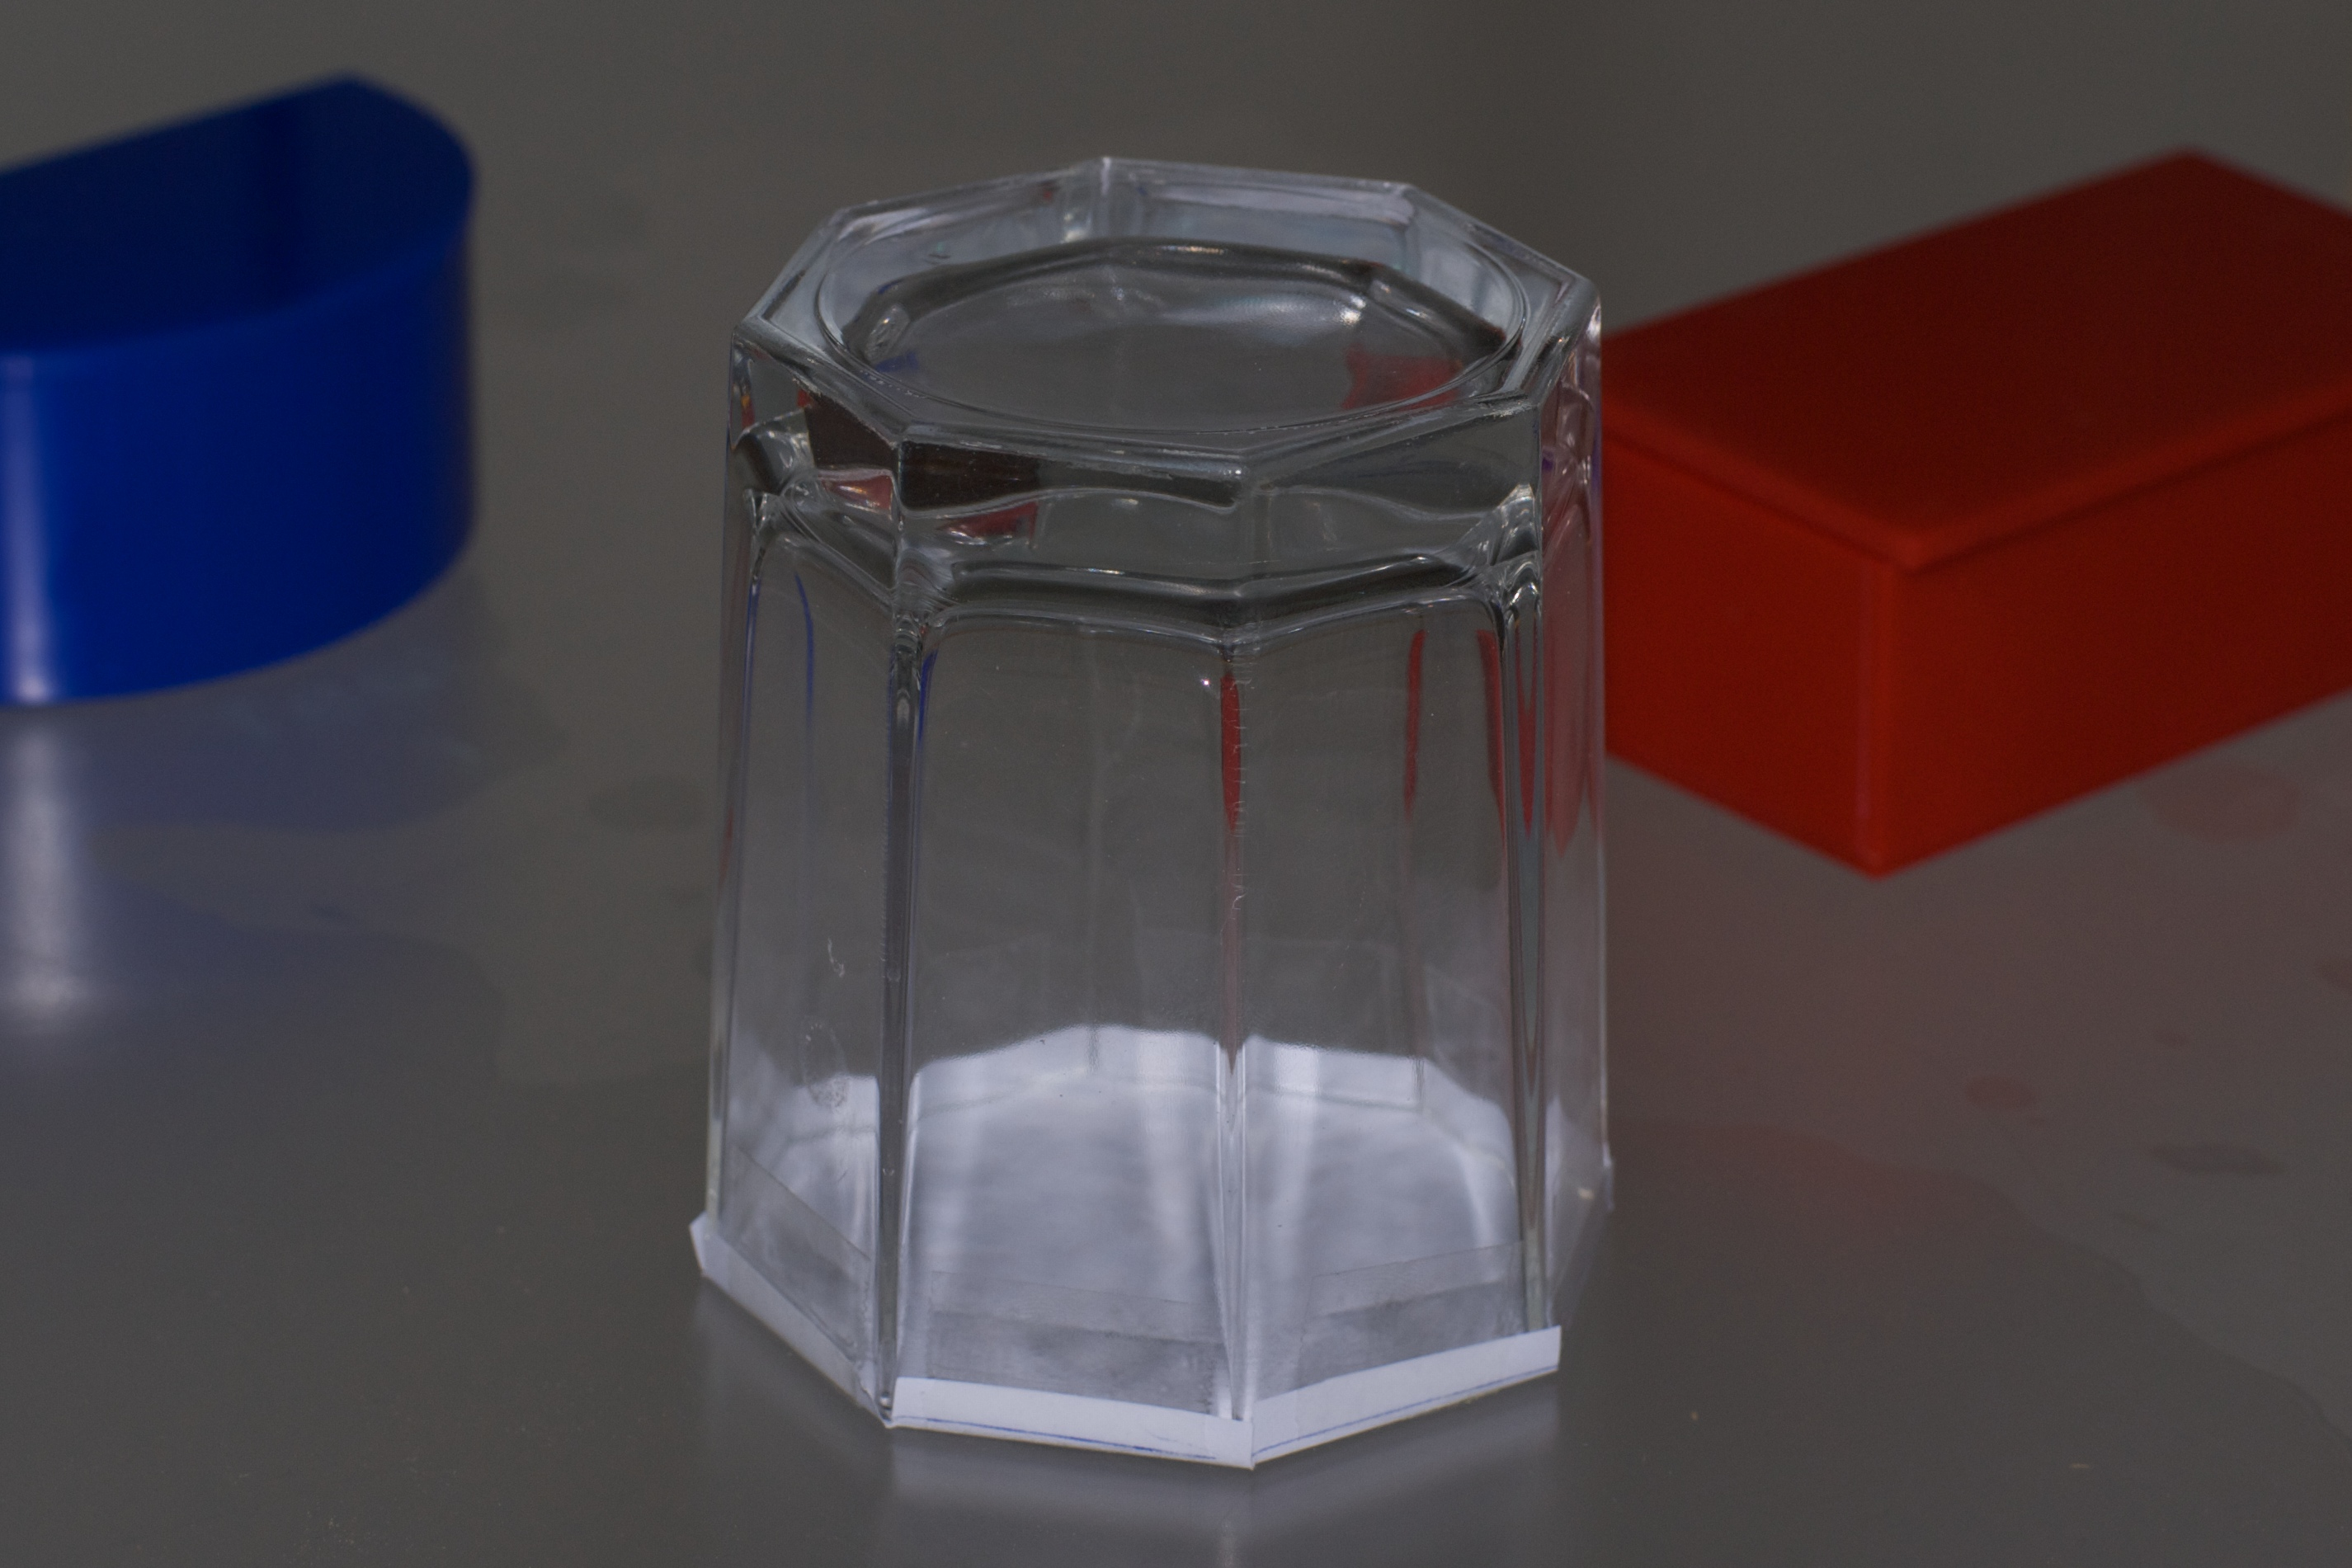
\includegraphics[height=2in]{img/SystemNeu/Historytoken.jpg}
	\caption{History-Token}
	\label{fig:img_SystemNeu_Historytoken}
\end{figure}

Das letze hier behandelte Token zur Steuerung einer Unterstützungsfunktion ist jenes, dass die in Kapitel XY als Anforderung definierte und in Kapitel XY im Detail beschriebene \emph{Wiederherstellungsunterstützung} auslöst. Die Verwendung dieses Tokens ist identisch mit jener des oben beschriebenen Snapshot-Tokens. Wie dieses ist es der ereignisauslösenden Kategorie zuzuordnen und aktiviert die Wiederherstellungsunterstützung wenn es bei aktivem Historien-Modus auf der Modellierungsoberfläche aufgesetzt wird. Die eigentliche Wiederherstellungsunterstützung ist dem Output-Kanal zuzuordnen und in ihrem Ablauf deshalb im Detail in Kapitel XY (Abschnitt XY) beschrieben.

% paragraph steuerung_von_unterstützungsfunktionen (end)
% subsubsection werkzeug_tokens (end)
% subsection tokens_&_input_werkzeuge (end)

\subsection{Eingabe auf der Tischoberfläche} % (fold)
\label{sub:input_auf_der_tischoberfläche}

Nachdem nun die Tokens beschrieben wurden, die den Benutzern unmittelbar zur Interkation mit dem System dienen, liegt der Fokus dieses Abschnitts nun auf der technischen Umsetzung der Erfassung der aktuell auf der Oberfläche sichtbaren ReacTIVision-Codes und damit der Tokens.

Wie bereits oben beschrieben, wurde bei der Umsetzung des optischen Tracking-Ansatzes eine Identifikation der Codes von der Unterseite gewählt, um etwaigen Erkennungsproblemen mit Verdeckungen vorzubeugen. Dies bedingt, dass die Modellierungsoberfläche für Kameras möglichst transparent sein muss um den Identifikationsvorgang nicht negativ zu beeinflussen. Grundsätzlich bietet sich dazu der Einsatz einer (Acryl-)Glasplatte an, die keinen Einfluss auf die Erfassung der auf ihr platzierten Codes hat. Der Einsatz einer (Acryl-)Glasplatte bringt jedoch zwei Probleme mit sich. Einerseits kann die Verwendung einer transparenten Oberfläche dazu führen, dass Modellierende durch den Einblick auf den inneren Aufbau des Systems von der Aufgabe abgelenkt bzw. irritiert werden. Andererseits verhindert eine transparente Oberfläche den Einsatz derselben als Rückkanal zur Darstellung von zusätzlicher Information durch einen Videoprojektor. Dies ist im konkreten Fall besonders schwerwiegend, da die a-priori unspezifischen Modellierungs-Tokens erst durch die Projektion der zusätzlichen Information explizit bedeutungstragend werden. Deswegen wurde eine semi-transparente Acrylglas-Oberfläche eingesetzt, die einerseits für die Erfassung der Codes ausreichend durchlässig ist, andererseits aber auch das projizierte Licht soweit bricht, dass die darzustellende Information auf der Oberfläche sichtbar ist.

Die Kamera -- eine AVT Guppy F080B \citep{AVT08}  -- sitzt wie in Abbildung \ref{fig:img_ImplementierungInput_TischSeitenansicht} schematisch dargestellt in der Mitte der Bodenplatte. Sie ist mit einem Weitwinkel-Objektiv ausgestattet, das es erlaubt, die gesamte Oberfläche zu erfassen, ohne dass der Tisch höher als 100 cm sein muss (Öffnungswinkel etwa 45°). Die Kamera bietet eine Auflösung von 1024 x 768 Bildpunkten und ist über eine Firewire-Schnittstelle (IEEE 1394 \citep{Bloks96}) mit dem Rechner verbunden. Die Kamera kann so bis zu 30 Bilder pro Sekunde an den Rechner senden. Das Weitwinkelobjektiv verursacht Verzerrungen in den Randbereichen, was trotz der Möglichkeit von ReacTIVision, das Bild softwareseitig zu entzerren, dazu führt, dass links und rechts etwa 10 cm der Tischoberfläche nicht zur Identifikation von Codes verwendet werden können. Dieser Problematik kann aufgrund der beschränkten Kameraauflösung nur durch größere Codes begegnet werden, was durch die beschränkte Größe der Tokens nicht möglich ist. Im Prototypen wurden deshalb die Randbereiche des Systems ausgespart und können zur Ablage von aktuell nicht eingesetzten Tokens verwendet werden. 

\subsubsection{Illumination und Umgebungslichtabhängigkeit} % (fold)
\label{sub:illumination_und_umgebungslichtabhängigkeit}

Optische Tracking-Systeme leiden generell unter ihrer Abhängigkeit von den Umgebungslichtbedingungen. Probleme, die in diesem Zusammenhang auftreten, hängen nicht nur mit der absoluten Stärke der Einstrahlung von Umgebungslicht zusammen (die zu schwach, aber auch zu stark sein kann), sondern auch mit der Änderung der Lichtbedingungen über die Zeit. Gegenstand dieses Abschnitts ist die genauere Erörterung dieser Problematik und die Darlegung von Möglichkeiten ihr zu begegnen.

Zu geringe Umgebungshelligkeit führt zu Erkennungsproblemen, da der Kamera nicht ausreichen Licht und damit Kontrast zur Verfügung steht, um ein Bild zu liefern, in dem die ReacTIVision-Codes zuverlässig identifiziert werden können (dies gilt im Übrigen auch für alle anderen optischen Identifikations-Ansätze). Das Problem wird zusätzlich verschärft, da zur Aufnahme des Bildes nicht das Spektrum des sichtbaren Lichts verwendet wird, sondern in den Infrarot-Bereich (“near infrared“, Wellenlänge etwa 550 nm) ausgewichen wird. Dies ist notwendig, da die Kamera andernfalls Reflexionen des auf die Oberfläche projizierten Output-Kanals (siehe Abschnitt XY) erfasst, was eine Identifikation der Codes unmöglich macht. Die meisten Kunstlicht-Quellen strahlen jedoch nicht ausreichend Licht im verwendeten Infrarot-Bereich ab, um eine ausreichende und gleichmäßige Ausleuchtung der Oberfläche zu gewährleisten. Dieser Problematik wurde dadurch begegnet, dass im betreffenden Infrarot-Bereich strahlende Beleuchtungsquellen in den Tisch (konkret in den Ecken der Bodenplatte) eingebaut wurden (siehe Abbildung \ref{fig:img_ImplementierungInput_TischSeitenansicht}). Um eine gleichmäßige, diffuse Ausleuchtung zu erreichen, wurde der Tisch rundum mit weißen Kunststoffplatten mit strukturierter Oberfläche verkleidet, die das vorhandene Licht streuen. Um Reflexionen der Lichtquellen (die nach oben abstrahlen) auf der Oberfläche zu vermeiden, wurden etwa 50 cm über den Lichtquellen Streuscheiben angebracht. So konnte eine diffuse Beleuchtungssituation geschaffen werden, deren Stärke ausreicht, um die Codes auch bei vollkommener Dunkelheit in der Umgebung zuverlässig zu erkennen.

Das zweite Problemfeld betrifft zu starke Lichteinstrahlung aus der Umgebung. Zu hohe Umgebungshelligkeit führt zu einem Überstrahlen des Kamerabildes in manchen Bereichen, womit in Teilen der Oberfläche keine Codes erkannt werden können. Dies liegt in dem von ReacTIVision eingesetzten adaptiven Code-Extraktions-Algorithmus begründet, der bei schwachen oder guten Beleuchtungsverhältnissen leichte Unterschiede in der Ausleuchtung korrigieren kann, bei starken Unterschieden oder großer Helligkeit jedoch nicht mehr zuverlässig funktioniert. Wie bereits erwähnt, arbeitet die Kamera im Infrarot-Bereich. Dies ist dann problematisch, wenn starke Sonneneinstrahlung vorhanden ist, da diese einen hohen Anteil an Lichts der relevanten Wellenlänge enthält. Auch bestimmte Kunstlichtquellen wie Leuchtstoffröhren, die unmittelbar über dem Tisch angebracht sind, verursachen Probleme. Während punktuelle Helligkeitszonen („Spotlights“) nicht durch die Software korrigiert werden können und vermieden werden müssen, kann eine generell zu hohe Umgebungshelligkeit durch die Kalibrierung der ReacTIVision-Software bzw. der ihr zugrunde liegenden Kamera-Treiber korrigiert werden. Im Konkreten ermöglicht ReacTIVision bei Firewire-Kameras eine Veränderung der Kamerablende (größere Blende -- weniger Licht am Sensor) sowie der Signalverstärkung (weniger Verstärkung -- dunkleres Bild). Durch Veränderung dieser beiden Parameter kann nahezu jede Beleuchtungssituation korrigiert werden, sofern sie über die Zeit stabil bleibt.

Bei Umgebungslicht-Bedingungen, die sich über die Zeit verändern (z.B. bei Tageslicht, das sich durch Wolkenbewegungen oder tageszeitabhängig verändert), kann die manuelle Konfiguration des ReacTIVision-Frameworks nicht sinnvoll durchgeführt werden. Leichte Veränderung der Helligkeit kann das ReacTIVision-Framework durch den adaptiven Erkennungs-Algorithmus noch selbst korrigieren, bei größeren Veränderungen funktioniert jedoch die Erkennung nicht mehr stabil. Dies äußert sich darin, dass Codes für einige Sekundenbruchteile von der Kamera nicht mehr erfasst werden, was wiederum zu unerwünschten von Framework gemeldeten Ereignissen führt (z.B. dass ein Container-Token verschwunden wäre, obwohl es sich physisch noch auf der Oberfläche befindet). Da diese Erkennungsausfälle im Grenzbereich gerade noch möglicher Erkennung zwar regelmäßig auftreten, in ihrer zeitlichen Ausdehnung aber eher kurz sind, wurde im Rahmen der Interpretation der vom ReacTIVision-Framework gemeldeten Ereignisse eine Stabilisierungsebene eingezogen, die versucht, Ausfälle und Fehlerkennungen zu identifizieren und dementsprechend nicht an die übergeordneten Software-Ebenen weiterzugeben. Die in dieser Ebene umgesetzten Maßnahmen sind in Abschnitt \ref{sub:stabilisierung_der_erkennungsleistung} beschrieben.

Durch die Kombination aller beschriebenen Maßnahmen ist es möglich, eine sehr weitgehende Einsetzbarkeit der Werkzeugs unabhängig von den herrschenden Umgebungslichtbedingungen zu gewährleisten. Lediglich bei extremen Verhältnissen wie direkter Einstrahlung von in der Stärke variierenden Lichtquellen verhindert einen stabilen Einsatz des Systems.  

% subsubsection illumination_und_umgebungslichtabhängigkeit (end)
% subsection input_auf_der_tischoberfläche (end)
% section konzeption_und_umsetzung_der_hardwarekomponenten (end)

\section{Benutzerinteraktion mit dem Werkzeug} % (fold)
\label{sec:benutzerinteraktion_mit_dem_werkzeug}

Bevor nun die Interpretation der Eingabedaten durch die Software beschrieben wird, muss vorab geklärt sein, auf welche Art und Weise Benutzer mit dem System interagieren können. Bisher wurde geklärt, wie die Eingabe technisch funktioniert und welche Elemente den Benutzern zur Interaktion mit dem System zur Verfügung stehen. Im Folgenden werden die einzelnen Aktionen, die Benutzer grundsätzlich im Kontext des Modellierungsablaufs setzen können, identifiziert und deren konkrete Umsetzung durch das vorgestellte System beschrieben.

Ein grundsätzliches Designziel war es, die Interaktion mit dem System so „natürlich“ wie technisch möglich zu gestalten. Unter „natürlich“ ist hier zu verstehen, dass 
\begin{itemize}
	\item die Eingabe von Information möglichst ausschließlich über direkte Aktionen der Hände der Benutzer (d.h. ohne Übersetzung in die digitale Welt durch Maus oder Tastatur) gestaltet werden kann, und
	\item dass diese Aktionen bzw. deren Ablauf nur durch inhaltliche Vorgaben der Modellierungsproblematik, nicht aber durch technische Einschränkungen, vorgegeben sind.
\end{itemize}
Wie bereits im letzen Abschnitt beschrieben, konnten diese Forderungen aufgrund der Eigenschaften des eingesetzten Tracking-Systems nicht vollständig umgesetzt werden. Wo noch Einschränkungen hinsichtlich der oben genannten Forderungen bestehen, wird in den folgenden Abschnitt darauf hingewiesen und ein möglicher Lösungsansatz skizziert.

\subsection{Hinzufügen und Verändern von Modellelementen} % (fold)
\label{sub:hinzufügen_und_verändern_von_modellelementen}

Um Elemente zu einem Modell hinzuzufügen müssen entsprechende Tokens auf der Modellierungsoberfläche platziert werden. Sofern sich diese im Erfassungsbereich der Kamera befinden, werden sie identifiziert und an der entsprechenden Stelle im Modell identifiziert. Beim erstmaligen Hinzufügen wird das Token dem Benutzern gegenüber mittels seiner Nummer (die durch den ReacTIVision-Code vorgegeben ist) dargestellt. Ist das Token bereits benannt und wird erneut hinzugefügt, wird die zuvor vergebene Benennung geladen und angezeigt.

Beim erstmaligen Hinzufügen eines Elementtyps (also eines roten, blauen oder gelben Tokens) fragt das System nach der Bedeutung dieses Elementtyps. Diese kann angegebenen werden, darf aber auch unspezifiziert bleiben und kann zu einem späteren Zeitpunkt festgelegt oder verändert werden. Diese Interaktion zu einem späteren Zeitpunkt muss explizit durch ausgelöst werden, indem ein Token des betreffenden Typs vor die Registrierungskamera gehalten wird.

Um die Position und Rotation eines Modellelements zu verändern, muss es entsprechend an einen anderen Ort verschoben oder gedreht werden. Dabei ist es nicht notwenig, dass das Token ständig von der Kamera erfasst wird. Kurze Aussetzer in der Erfassung, die durch schnelles Verschieben oder Abheben des Tokens und Aufsetzen an einem anderen Ort ausgelöst werden, werden von der Software ignoriert, das Element wird so behandelt, als wäre es nicht verschwunden gewesen (hinsichtlich der Auswirkungen des Verschwindens eines Tokens siehe Abschnitt \ref{sub:löschen_von_elementen}).

Eine simultane Erweiterung oder Veränderung des Modells durch mehrere Benutzer ist möglich, die Software schränkt die Anzahl der möglichen zeitgleich ablaufenden Interaktionen nicht ein. Da alle in diesem Abschnitt beschriebenen Interaktionen eindeutig einem Token zugeordnet werden können und dieses zu jedem Zeitpunkt eindeutig identifiziert werden kann, kann das System mit dieser Art von Eingaben umgehen. Die Erfassungsrate liegt in der derzeitigen Implementierung bei etwa 15 Bildern in der Sekunde, woraus sich ein Auswerteintervall von etwa 67 Millisekunden ergibt. In diesem Abstand wird jeweils die gesamte Oberfläche erfasst und etwaige Änderungen an die Applikationsschicht weitergemeldet.
 
% subsection hinzufügen_und_verändern_von_modellelementen (end)

\subsection{Benennen von Modellelementen} % (fold)
\label{sub:benennen_von_modellelementen}

Die Benennung von Modellelementen ist eine der wichtigsten Interaktionsformen im Modellierungsprozess. Modellelementen wird damit ein Name zugewiesen, der zur Identifikation des Elements gegenüber den Benutzern verwendet wird. Um der Anforderung nach möglichst direkter, unmittelbarer Interaktion mit dem System in der realen Welt (d.h. auf der Modellierungsoberfläche) nachzukommen, wurde ein auf der Verwendung von Haftnotizen basierender Interaktionsmodus eingeführt, der zur Benennung von Modellelementen eingesetzt wird. Alternativ kann die Benennung durch Eingabe der Bezeichnung über eine Tastatur erfolgen.

Im Falle der Benennung mittels Haftnotizen wird ein Werkzeugtoken eingesetzt, auf dem die Haftnotizen angebracht sind. Unmittelbar nach der Platzierung eines Elements wird eine neue Haftnotiz beschriftet und mittels der Registrierungskamera erfasst. Während die Haftnotiz nun auf dem Modellelement angebracht werden kann, wird im System das erfasste Bild ausgewertet, der geschriebene Text wird (als Grafik) extrahiert und dem zuletzt auf der Oberfläche platzierten Token zugeordnet. Soll ein Element nachträglich (um)benannt werden -- wenn also zwischenzeitlich ein weiteres Element platziert wurde -- muss das zu benennende Element mit dem Markierungstoken ausgewählt werden. Das Markierungstoken wird dazu in der Nähe des Elements auf die Oberfläche gesetzt. Visuelles Feedback auf der Oberfläche signalisiert eine erfolgreiche Auswahl. In der Folge kann die neue Benennung mittels des Registrierungstokens erfasst und am Element angebracht werden. Die Benennung mittels Haftnotizen ist insofern problematisch, als dass die Extraktion der handschriftlichen Benennung nur unzuverlässig funktioniert. Dies liegt vor allem an zu geringem Kontrast zwischen Haftnotiz und Schrift ( bei schlechten Lichtverhältnissen) und einer zu geringen Auflösung der Registrierungskamera. Außerdem werden keine Schrifterkennungs-Algorithmen eingesetzt, wodurch der Schriftzug für das System immer lediglich eine Menge von Bildpunken ohne weitere Bedeutung bleibt.

Um die Nachteile der Benennung mit Haftnotizen zu vermeiden, wurde ein alternativer Interaktionsmodus zur Benennung von Modellelementen eingeführt. Dieser läuft grundsätzlich identisch ab, setzt jedoch anstatt der Haftnotizen eine Tastatur ein, über die die Benutzer die Benennung dem System bekannt geben. Die eingegebene Information wird dann auf der Oberfläche unmittelbar unterhalb des Elements angezeigt (siehe Kapitel XY). Die Auswahl des zu benennenden Elements erfolgt wiederum durch das Markierungstoken. Die Vorteile dieses Systems liegen in der geringen Fehlerrate und der hohen Geschwindigkeit der Eingabe (etwa Faktor 10 schneller als die Eingabe mittels Haftnotiz). Der Nachteil dieses Ansatzes ist der exklusive Zugang zum Eingabemedium, der Tastatur. Während es beim Einsatz von Haftnotizen grundsätzlich möglich ist, diese simultan zu erstellen (auch wenn die Registrierung sequentiell erfolgen muss), kann bei der Verwendung der Tastatur zu einem Zeitpunkt immer nur ein Element bearbeitet werden.

Grundsätzlich sind die beiden Interaktionsmodi zur Benennenung von Elementen als Ergänzung zueinander zu sehen. Sie können grundsätzlich gleichzeitig eingesetzt werden und bieten den Benutzern eine Wahlmöglichkeit zwischen einer langsameren, dafür aber physisch existenten oder einer schnelleren, dafür nur über die Ausgabekanäle des Systems sichtbaren Benennung. Die Erkennungsprobleme der Haftnotizen-Variante (die zur Einführung des zweiten Interaktionsmodus geführt hatten) können durch eine Verbesserung der technischen Rahmenbedingung ausgemerzt werden, wozu aber bei der Erstellung des hier vorgestellten Prototypen keine Ressourcen vorhanden waren. Im Falle einer Verbesserung könnten den Benutzern zwei gleichwertige Eingabekanäle zur Verfügung gestellt werden. Vorerst bietet der Einsatz der Tastatur jedoch nicht vernachlässigbare Vorteile hinsichtlich der Zuverlässigkeit und der Genauigkeit der Erfassung von Benennungen.

% subsection benennen_von_modellelementen (end)

\subsection{Verbinden von Modellelementen} % (fold)
\label{sub:verbinden_von_modellelementen}

Das Verbinden von Modellelementen ist neben dem Hinzufügen und Benennen der dritte wesentliche Interaktionsmodus, der zum Aufbau eines Modells benötigt wird. Verbindungen werden nicht physisch gelegt sondern mit Werkzeugtokens erstellt und dann über die Outputkanäle visuell dargestellt. Die Entscheidung gegen eine physische Repräsentation der Verbindungen fiel zugunsten einer leichteren Veränderbarkeit des gesamten Modells -- das Verschieben eines Elements verursacht so keinen zusätzlichen Aufwand, wohingegen physische Verbinder nachgeführt werden müssten bzw. eine beliebige Neuanordnung verhindern würden.

Die Erstellung von Verbindern kann wie die Benennung auf zwei unterschiedliche Arten erfolgen, die sich aber ihrer Ausdrucksmächtigkeit bzw. Flexibiliät unterscheiden. Der flexiblere Interaktionsmodus ist jener, der unter Einsatz von zwei Markierungstokens durchgeführt wird. Dabei wird jeweils ein Markierungstoken neben einem der beiden zu verbindenden Modellelemente platziert, wodurch diese ausgewählt und anschließend verbunden werden. Das Verbindungskriterium ist, dass die beiden Modellelemente innerhalb von 3 Sekunden nacheinander ausgewählt werden. Dies erlaubt sowohl eine gleichzeitige Platzierung von zwei Markierungstokens als auch die Arbeit mit nur einem Token, das rasch hintereinander neben die zu verbindenden Elemente gesetzt wird. Die Arbeit mit den herkömmlichen Markierungstokens erzeugt ungerichtete Verbindungen. Werden gerichtete Verbindungen benötigt (deren Richtung mit einer oder im Falle einer bidirektionalen Verbindung mit zwei Pfeilspitzen angezeigt wird), müssen spezielle Markierungstokens verwendet werden, deren Grundfläche die Form einer Pfeilspitze hat und die neben dem entsprechend zu markierenden Modellelemente platziert werden müssen.

Der alternative Interaktionsmodus zur Herstellung einer Verbindung kommt ohne Werkzeugtokens aus und basiert ausschließlich auf der Manipulation der Modellelemente. Werden zwei Modellelement an ihren Längsseiten nahe zusammengeführt, so erstellt das System zwischen diesen beiden Elementen eine Verbindung. Im Interaktionsablauf bedeutet dies, dass ein Benutzer die beiden zu verbindenden Elemente ergreift und diese auf der Oberfläche von ihrer ursprünglichen Position aus kurz zusammenführt um sie danach sofort wieder an ihre Originalposition zurück zu stellen. Die so erstellten Verbindungen sind immer ungerichtet und werden nach der Erstellung gleich behandelt wie mit den Markierungstokens erstellte Verbindungen. Durch die Vermeidung der Verwendung von Werkzeugtokens ist dieser Weg zur Herstellung von Verbindungen schneller auszuführen als der zuvor beschriebene (etwa um den Faktor 5). Problematisch wird diese Art der Interaktion dann, wenn die Modellierungsoberfläche bereits sehr voll ist, so dass nur noch wenig Platz zur Zusammenführung von zwei Elementen vorhanden ist. Auch bei Bedarf nach gerichteten Verbindern muss auf Markierungstokens zurückgegriffen werden.

Markierungen können unabhängig von ihrem Erstellungsweg auch benannt werden. Da sie keine physische Repräsentation besitzen, kann der Benennungsmodus mit Haftnotizen nicht verwendet werden. Die Eingabe von Bezeichnungen erfolgt demnach ausschließlich über die Tastatur. Zur Benennung einer Verbindung muss unmittelbar nach deren Erstellung die Bezeichnung eingegeben werden, diese wird dann der zuletzt erstellten Verbindung zugewiesen. Um eine Bezeichnung zu ändern oder im Nachhinein zuzuweisen, muss der Verbinder mittels dem Markierungstoken ausgewählt werden. Durch nachträgliches Aufsetzen des Pfeilspitzen-Tokens auf eine existierende Verbindung wird am jeweils näheren Verbindungsende eine Pfeilspitze hinzugefügt oder entfernt werden.
% subsection verbinden_von_modellelementen (end)

\subsection{Löschen von Elementen und Verbindungen} % (fold)
\label{sub:löschen_von_elementen}

Beim Löschen muss zwischen dem Entfernen von Elementen und Verbindungen unterschieden werden. Beide Modellaspekte sind nicht nur hinsichtlich der Interaktion mit dem System unterschiedlich zu behandeln, es besteht vor allem eine Existenzbeziehung zwischen Elementen und Verbindungen, d.h. dass Verbindungen nicht ohne ihre als Endpunkte dienenden Elemente existieren können und beim Entfernen eines Elements ebenfalls gelöscht werden müssen.

Das Löschen eines Modellelements aus dem aktuellen Modell erfolgt durch Entfernen der zugehörigen Tokens auf der Oberfläche. Hier muss zwischen Entfernungsvorgängen unterschieden werden, die vom Benutzer intendiert sind und solchen, die durch die Manipulation des Modells unabsichtlich und kurzzeitig auftreten. Nur in ersterem Fall dürfen die Verbindungen, die an einem Element hängen, ebenfalls gelöscht werden. Die Unterscheidung zwischen den beiden Fällen wurde durch die Einführung eines Zeitintervalls von 5 Sekunden gelöst, nachdem die betroffenen Verbinder ebenfalls entfernt werden. Wird also ein Modellelement nur an eine andere Stelle verschoben (und verschwindet so kurzzeitig aus dem Blickfeld der Kamera), bleiben die Verbindungen erhalten. Wird das Element zur Seite gestellt, wird es und seine abhängigen Verbindungen zwar auf den Ausgabekanälen nicht mehr dargestellt, das tatsächliche Löschen erfolgt aber erst nach 5 Sekunden. Wird das Element innerhalb dieser Zeitspanne wieder auf der Oberfläche platziert, wird es und seine abhängigen Verbindungen so behandelt, als ob es nicht verschwunden gewesen wäre.

Das Löschen von Verbindern ist durch den Einsatz der Lösch-Tokens möglich, dass das System in den Lösch-Modus schaltet sobald es auf der Oberfläche platziert wird (und diesen wieder deaktiviert, wenn es entfernt wird). Im Lösch-Modus wird der Einsatz von Markierungstokens alternativ interpretiert. Anstatt der Herstellung einer Verbindung wird bei Markierung von zwei Modellelementen eine eventuell zwischen diesen vorhandene Verbindung endgültig entfernt. Dabei ist keine Unterscheidung zwischen gerichteten und ungerichteten Verbindungen notwendig, es können durchgängig die einfachen Markierungstokens eingesetzt werden.

% subsection löschen_von_elementen (end)

\subsection{Einbettung von Zusatzinformation} % (fold)
\label{sub:einbettung_von_zusatzinformation}

Der Interaktionsablauf zur Einbettung von Zusatzinformation setzt sich aus zwei Teilen zusammen, die sequentiell abzuarbeiten sind. Der erste Schritt ist der Vorgang des Bindens von Zusatzinformation an ein einbettbares Token. Im zweiten Schritt muss dieses Token in einem Container-Token eingebettet werden. Ein dritter Interaktionsablauf in diesem Zusammenhang ist das Abrufen  bzw. die Manipulation der eingebetteten Information, der in der Folge ebenfalls im Detail beschrieben wird.

Das Binden von Information an ein einbettbares Token ist ein Vorgang, der nicht ausschließlich in der physischen Welt durchgeführt werden kann. Die anzubindende Information liegt im Regelfall digital vor und muss damit am Rechner selektiert werden. Der zugehörige Informationsablauf beginnt mit der Auswahl eines einbettbaren Tokens, dessen Form die Art der einzubettenden Information bestimmt. Im konkreten Fall wurden drei Arten von einbettbaren Tokens erstellt, von denen eines der Umsetzung der Abstraktion von Modellen (also der Einbettung von Teilmodellen in ein Containerelement) dient und die anderen beiden exemplarisch die Anbindung von digitalen Ressourcen aus der Arbeitsumgebung demonstrieren. Im Sinne des Interaktionsablaufs sind diese Arten zum Teil unterschiedlich zu behandeln. Bei allen Token startet die Interaktion mit der Registrierung des Tokens mittels der Registrierungskamera. Handelt es sich dabei um ein Token, das der Einbettung von Teilmodellen dient, wird der aktuelle Modellzustand auf der Modellierungsoberfläche erfasst, gespeichert und an das Token gebunden. Der Vorgang der Informationsanbindung ist in diesem Fall abgeschlossen. Daneben existieren Tokens, an die beliebige digitale Ressourcen in der Form von Dateien gebunden werden können. Die Registrierung eines derartigen Tokens öffnet in diesem Fall eine Dialogbox am Rechner, in der die digitale Ressource ausgewählt werden kann. Die gewählte Datei wird dann über eine Referenz an das Token gebunden. Die dritte Art von einbettbaren Tokens demonstriert die Anbindung von spezialisierterer Information, die in einem Anwendungsfall sinnvoll sein können und ggf. auch gesondert behandelt werden müssen. Im konkreten Fall wurde die Anbindung von unmittelbar aufgenommenen Bildern implementiert, die so z.B. eine Abbildung eines Ausschnittes der realen Arbeitsumgebung in das Modell ermöglichen. Im Interaktionsablauf löst die Registrierung eines derartigen Tokens die Speichung eines Bildes, das aktuell von der Registrierungskamera erfasst wird, aus. Dieses Bild wird an das Token gebunden, der Interaktionsablauf ist damit ebenfalls wieder beendet.

Im zweiten Schritt, der zur Einbettung von Information notwendig ist, muss das einbettbare Token einem Containertoken zugeordnet werden. Dazu muss das betreffende Container-Token geöffnet werden. Das einbettbaren Token, an das bereits Information gebunden wurde, wird erneut mit der Registrierungskamera erfasst, was eine Zuordnung zwischen diesem Token und dem offenen Container auslöst. Visuelles Feedback über die Ausgabekanäle zeigt eine erfolgreiche Zuordnung an. Das einbettbare Token kann nun auch physisch in den Container gelegt werden und ist diesem damit auch in der realen Welt zugeordnet. Der Interaktionsvorgang endet mit dem Schließen des Containertokens. Der hier beschriebene Vorgang ist insofern als Hilfskonstrukt zu sehen, als das er nicht notwendig wäre, wenn die Containertoken in der Lage wären, ihren Inhalt selbst zu identifizieren. Wie in Abschnitt \ref{ssub:tokenzustand} argumentiert, wurde aber auf diese Funktionalität verzichtet. Dies ist für den prototypischen Einsatz akzeptabel, im Realbetrieb jedoch insofern problematisch, als dass durch den indirekten, mehrstufigen Zuordnungprozess ein inkonsistenter Zustand zwischen physischer und digitaler Modellrepräsentation nicht ausgeschlossen werden kann.

Um eingebettete Information wieder abrufen zu können, wurde ebenfalls ein Interaktionsablauf definiert. Dieser beginnt mit dem Öffnen des entsprechenden Container-Tokens. Durch Herausnehmen des informationstragenden Tokens und eine Erfassung desselben mit der Registrierungskamera wird die angebundene Information abgerufen. Handelt es sich um ein Token mit angebundenen Teilmodell, so wird dieses über die Output-Kanäle dargestellt. Angebundene digitale Ressourcen werden am Rechner geöffnet und dargestellt. Das eingebettete Token bleibt dem Container-Token zugeordnet, es muss also zur Konsistenzsicherung nach dem Abrufen der Information wieder in den Container gelegt werden. Um ein eingebettetes Token aus einem Container zu entfernen, muss bei der Erfassung dieses Tokens das Radierer-Werkzeug-Token eingesetzt werden und das System so in den Lösch-Modus versetzt werden. Die Information bleibt dabei an das einbettbare Token gebunden. Eine Veränderung der angebundenen Information während eines Modellierungsvorgangs ist nicht vorgesehen, es muss ggf. ein weiteres, noch unbelegtes einbettbares Token verwendet werden. 

% subsection einbettung_von_zusatzinformation (end)

\subsection{Kontrolle der Modellierungshistorie} % (fold)
\label{sub:kontrolle_der_modellierungshistorie}

Die Kontrolle der Modellierungshistorie umfasst im Wesentlich drei Interaktionsblöcke, die im Folgenden beschrieben werden. Der erste Block behandelt die Erfassung von Modellzuständen, im zweiten Block wird die Navigation durch die Modellierungshistorie behandelt und der dritte Block beschäftigt sich mit der Unterstützung der Wiederherstellung von gespeicherten Modellzuständen.

Die Erfassung von Modellzuständen erfolgt im Normalfall implizit und muss von den Benutzern nicht explizit ausgelöst werden. Wenn sich das Modell auf der Modellierungsoberfläche länger als 5 Sekunden in einem stabilen Zustand befinden (wenn also weder die Position, noch die Rotation oder die Benennung der Tokens geändert wurden und auch keine Verbindungen oder Einbettungen erstellt wurden), wird der aktuelle Modellzustand gespeichert. Sollen bestimmte Modellzustände aber aufgrund ihrer Relevanz für den Modellierungsverlauf explizit gespeichert und auch entsprechend gekennzeichnet werden, so kann das Snapshot-Token eingesetzt werden. Dieses löst sobald es auf der Modellierungsoberfläche aufgesetzt wird die Speicherung des aktuellen Modellzustandes aus. Das System quittiert die Speicherung mit visuellem Feedback über die Ausgabekanäle. Explizit erfasste Zustände werden im Gegensatz zu automatisch gespeicherten gekennzeichnet und in den weiterverarbeitenden Modulen (vor allem bei der Persistierung) speziell behandelt.

Die Navigation durch die Modellierungshistorie erfolgt mittels einem runden Werkzeug-Token, dass diese Navigation durch Rotation im oder entgegen dem Uhrzeigersinn ermöglicht. Das System wird durch das Aufsetzen dieses Tokens auf die Modellierungsoberfläche in den Historien-Modus geschaltet, was Auswirkungen auf die Darstellung des Modells in den Outputkanälen (siehe Abschnitt XY) hat. Bei Aktivierung des Historien-Modus wird der aktuellste gespeicherte Modellzustand geladen. Durch Drehen des Tokens gegen den Uhrzeigersinn kann in der Zeit zurück navigiert werden. Das Laden der nächstälteren Modellzustands erfolgt dabei in regelmäßigen Intervallen von jeweils 45 Grad (8 Modellzustände pro voller Umdrehung). Der absolute zeitliche Abstand zwischen den gespeicherten Modellzuständen, der sich aus dem Auftreten stabiler Modellzustände ergibt, wird bei der Navigation nicht berücksichtigt -- der zurückzulegende Winkel ist immer gleich groß. Gleiches gilt sinngemäß für das Drehen des Tokens im Uhrzeigersinn -- dabei wird in regelmäßigen Abständen der nächstjüngere Modellzustand geladen. Wird das Token entfernt, wird der Historien-Modus deaktiviert und wieder in der aktuelle Systemzustand an die Output-Kanäle übergeben.

Soll ein gespeicherter Modellzustand wiederhergestellt werden, so bietet das System Unterstützung für die dazu notwendige Interaktion. Da weder die Tokens noch der Tisch selbst über durch den Rechner steuerbare bewegliche Komponenten verfügen, die eine automatisierten Wiederherstellung eines Modellzustandes ermöglichen würden, kommt die Aufgabe der eigentlichen Wiederherstellung den Benutzern zu. Das System unterstützt dabei insofern, als das über die Ausgabekanäle Information an die Benutzer weitergegeben wird, die die korrekte Platzierung der Elemente anleitet (Details dazu sind in Abschnitt XY nachzulesen). Gespeicherte Modellzustände können dabei entweder aus dem Historienmodus oder aus an eingebettete Tokens gebundene Teilmodelle bezogen werden. Im ersten Fall wird die Wiederherstellungsunterstützung durch ein spezielles Token aktiviert, das auf die Oberfläche aufgesetzt wird während der alte Systemzustand über die Outputkanäle dargestellt wird. Im zweiten Fall muss das Teilmodell, das an das eingebettete Token gebunden ist, über die Registrierungskamera abgerufen werden, wodurch es ebenfall über die Outputkanäle dargestellt wird. Während der Darstellung wird die Wiederherstellungsunterstützung wiederum durch Aufsetzen des betreffenden Werkzeug-Tokens auf die Oberfläche aktiviert. In beiden Fällen läuft dann die Wiederherstellungsunterstüztung durch das System angeleitet automatisiert ab. Nach Abschluss der Wiederherstellung werden die Benutzer aufgefordert eventuell noch vorhandene Werkzeug-Tokens (wie das Historien-Navigations-Token) zu entfernen, wodurch das System wieder den aktuellen Modellzustand als Grundlage der Darstellung verwendet.
 
% subsection kontrolle_der_modellierungshistorie (end)
% section benutzerinteraktion_mit_dem_werkzeug (end)


\section{Erfassung der Benutzerinteraktion durch Software} % (fold)
\label{sec:erfassung_der_benutzerinteraktion_durch_softfware}

Das Software-System, das die Benutzereingaben von der Hardwareschnittstelle bis hin zur abstrahierten Modellierungsinformation aufbereitet, ist Gegenstand dieses Abschnitts. Die darüber hinausgehenden Komponenten sind Gegenstand der Kapitel X und Y. Die hier behandelten Software-Komponenten umfassen
\begin{itemize}
	\item jene Komponente, die die Rohdaten von ReacTIVision empfängt und sie hinsichtlich der Modellierungsinformation auswertet und interpretiert,
	\item die Komponente, die für die Stabilisierung der Erkennungsleistung sorgt, wenn Fehlerkennung oder Erkennungsausfälle auftreten, sowie
	\item jene Komponente, die für das Tracking des Modellzustandes und damit für die Nachvollziehbarkeit des Modellierungsablaufs zuständig ist. 
\end{itemize}
Wie in Abschnitt \ref{subs:vergleich_generische_frameworks} ausgeführt, soll zur Verknüpfung dieser Komponenten das TUIpist-Framework zum Einsatz kommen. Im vorliegenden Prototypen wurde das System jedoch zwar modular aber ohne Einsatz des TUIpist-Frameworks implementiert. Eine erste Umsetzung der Architektur auf die TUIpist-Strukturen liegt vor, ist jedoch noch nicht im produktiven Einsatz. An dieser Stelle wird deshalb der Aufbau der Komponenten in ihrer derzeitigen Implementierung beschrieben, da diese auch bei der Evaluierung des Werkzeugs eingesetzt wurde. Erste Umsetzungserfahrungen deuten darauf hin, dass der Aufwand zur Einbindung von TUIpist sich wie erwartet in Grenzen hält.

Die Systemarchitektur, wie sie sich in der derzeitigen Implementierung darstellt ist in Abbildung \ref{fig:img_ImplementierungInput_InputArchitecture} dargestellt. Die Komponenten des Interpretations-Moduls leiten sich aus den umzusetztenden Funktionen und zu erkennenden Interaktionsabläufen (siehe Abschnitt \ref{sec:benutzerinteraktion_mit_dem_werkzeug}) ab. Die Komponenten sowie die Verknüpfungen untereinander werden in den folgenden Abschnitten im Detail beschrieben, wobei die Struktur der Beschreibung im Gegensatz zum vorangegangenen Abschnitt nicht an der Funktionalität sondern an den involvierten Technologien orientiert ist und damit einen weiteren Detaillierungsschritt in der Beschreibung der Benutzereingabe im hier vorgestellten System darstellt.

\begin{figure}[htbp]
	\centering
		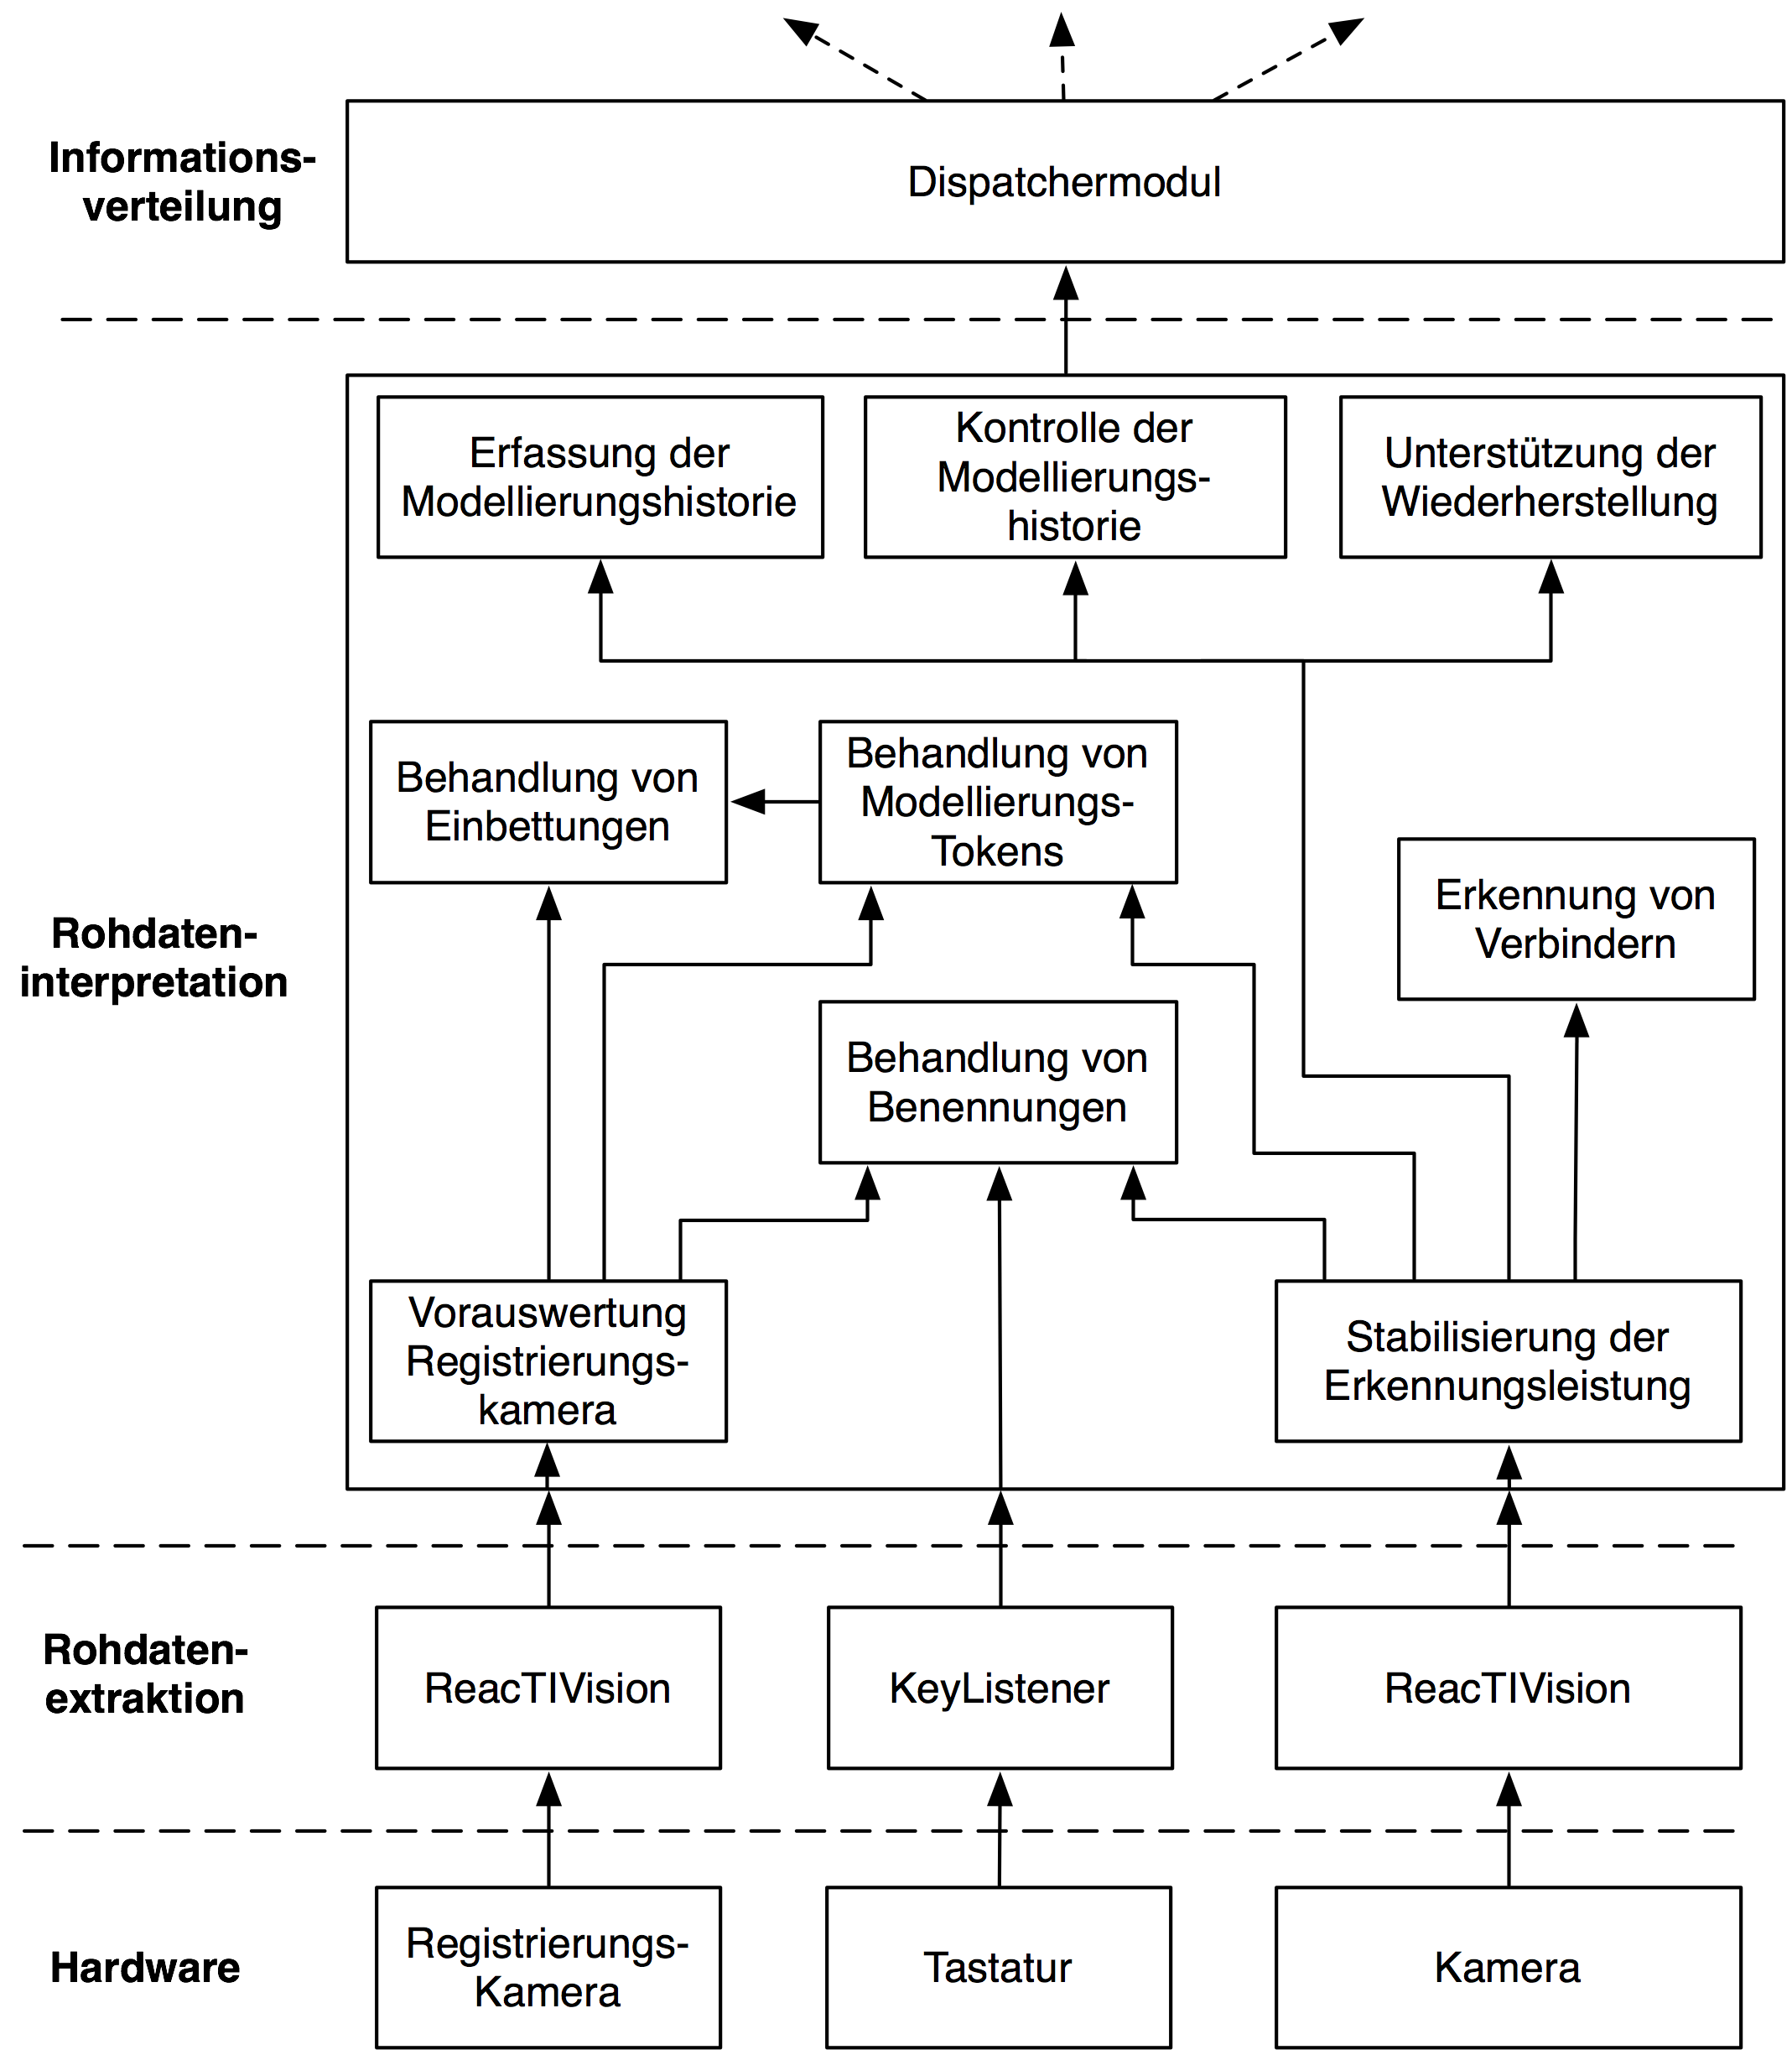
\includegraphics[width=15cm]{img/ImplementierungInput/InputArchitecture.png}
	\caption{Softwarearchitektur zur Erkennung von Benutzerinteraktion}
	\label{fig:img_ImplementierungInput_InputArchitecture}
\end{figure}

% section erfassung_der_benutzerinteraktion_durch_software (end)

\subsection{Interpretation der Rohdaten} % (fold)
\label{sub:interpretation_der_rohdaten}

Das ReacTIVision-Framework liefert wie in Abschnitt \ref{par:reactivision} beschrieben die aus dem Kamerabild extrahierten Informationen über die ausan. Für jeden erkennbaren Code wird eine separate Nachricht gesandt, sobald sich zumindest ein Parameter (also Position oder Rotation) verändert. Diese Nachrichten treffen über die UDP-Schnittstelle bei einem von ReacTIVision bereitgestellten Java-Objekt ein, das die Auswertung der Nachricht übernimmt und über einen Callback-Mechanismus\footnote{entsprechend dem in \citep{Gamma95} beschriebenen Beobachter-Muster (Observer), das bei der Entwicklung wiederverwendbarer objektorientierter Software als Entwurfsmuster zum Einsatz kommt} vom Anwendungsentwickler implementierte Methoden aufruft, die auf das jeweilige Ereignis reagieren. Die Ereignisse, die auftreten können, beschränken sich auf das Erscheinen eines Tokens, die Änderung der Parameter eines Tokens und das Verschwinden eines Tokens sowie die gleichen drei Ereignisse für die Behandlung eines Cursors (wie das Markierungs-Werkzeugtoken). Dazu werden jeweils die relevanten Parameter zur Verfügung gestellt (im Wesentlichen die ID des Tokens, seine Position, seine Rotation und einige weitere abgeleitete Parameter, die in der konkreten Anwendung nicht eingesetzt werden).

In den betreffenden Methoden wird im ersten Schritt ausgewertet, ob das identifizierte Token ein Modellierungs-Element oder ein Werkzeug ist. Im Falle eines Modellierungs-Elements wird im nächsten Schritt festgestellt, um welche Art von Token es sich handelt und ob es im aktuellen Modellierungsvorgang bereits im Einsatz war (ob z.B. bereits Information über die Benennung des Tokens oder dessen Inhalt vorhanden ist). Diese Information wird ggf. geladen und den weiterverarbeitenden Komponenten zu Verfügung gestellt. Im Falle eines Werkzeug-Tokens wird dieses identifiziert und an die für die Behandlung zuständige Methode weitergeleitet. Diese Methoden schalten das System je nach Art des eingesetzten Tokens in einen alternativen Zustand oder lösen eine Aktion auf den übergeordneten Ebenen aus.

Ist für die Interpretation einer Benutzerinteraktion mehr als ein Token notwendig (z.B. beim Ziehen von Verbindungen), werden die Kandidaten, die möglicherweise den Beginn einer derartigen Interaktionssequenz darstellen in einen Buffer geschrieben. Beim Auftreten eines Tokens, das möglicherweise den zweiten Teil dieser Interaktion darstellt, wird dieser Buffer geprüft und die Interpretation ggf. auf Basis der gespeicherten und aktuellen Token-Daten durchgeführt.

Manche Benutzereingaben müssen -- um eine komfortable Erstellung des Modells zu ermöglichen -- ggf. auch nach Entfernen eines Tokens für einen bestimmten Zeitraum gespeichert werden. Beispiele hierfür sind Markierungen, die auch nach Entfernen des Markierungstokens aktiv bleiben um Zeit für die Benennung oder die Herstellung einer Verbindung zu geben oder auch Modellierungstoken, die durch Manipulation temporär aus dem Erkennungsbereich der Kamera geraten und in diesem Fall nicht sofort als „entfernt“ interpretiert werden sollen. Auch in diesem Fall werden Buffer eingesetzt, die die entsprechende Information mit einem Zeitstempel versehen aufnehmen. Zur Sicherstellung der Modellkonsistenz (also der Übereinstimmung zwischen physischem und digitalem Modell) prüfen speziell dazu konzipiert Methoden, die von einem Timer in regelmäßigen Abständen aufgerufen werden, ob die vorgegebene Gültigkeitsdauer der Information bereits abgelaufen ist und entfernen diese ggf. endgültig aus dem Buffer und dem Modell (löschen also konkret eine Markierung oder entfernen ein Modellelement und alle abhängigen Verbindungen aus dem Modell). Die Zeitintervalle dieser Prüfungen sind auf den jeweiligen Anwendungsfall abgestimmt und bewegen sich im Bereich zwischen drei und fünf Sekunden.

% subsection interpretation_der_rohdaten (end)

\subsection{Stabilisierung der Erkennungsleistung} % (fold)
\label{sub:stabilisierung_der_erkennungsleistung}

Da wie bereits beschrieben beim Einsatz von ReacTIVision bei grenzwertigen Beleuchtungsbedingungen zu Erkennungsproblemen oder Fehlerkennungen neigt, wurden im Programmcode des Interpretationsmoduls Mechanismen verankert, die potentielle Fehlerkennungen und Erkennungsprobleme identifizieren und deren Auswirkungen ignorieren sollen. Im Folgenden werden häufige Fehlerquellen benannt und der jeweilige Lösungsansatz beschrieben.

\subsubsection{Bildrauschen} % (fold)
\label{ssub:bildrauschen}

Bei wenig vorhandenem Umgebungsumgebungslicht müssen die Kameraparameter wie oben bereits beschrieben soweit nachgeführt werden, bis wieder ausreichender Bildkontrast vorhanden ist. Zur Nachführung eignen sich die Blende der Kamera und die Signalverstärkung. Eine offene Blende erhöht den Lichteinfall auf den Sensor und verbessert damit die Bildhelligkeit und den Kontrast. Je weiter offen die Blende eingestellt ist, desto geringer ist jedoch auch die Tiefenschärfe des Kamerabilds, d.h. dass die Kamera sehr exakt auf die Modellierungsoberfläche fokussiert werden muss. Da der Abstand von der Kamera zu Mitte des Tisches geringer ist als zu den Randbereichen, kann bei offener Blende nie die gesamte Oberfläche scharf eingestellt werden. Da ein unscharfes Bild die Erkennungsleistung massiv mindert, sind der Nachführung des Blenden-Parameters Grenzen gesetzt. Die Signalverstärkung wirkt demhingegen nicht direkt auf die Kamera sondern auf das von ihr gelieferte Bild und ist deswegen keine physikalischen Beschränkungen unterworfen. Bei der Erhöhung der Signalverstärkung werden helle Bereiche im Bild heller, dunkle bleiben eher dunkel, der Kontrast wird also erhöht. Problematisch ist in diesem Kontext, dass nicht nur das Nutzsignal (also das eigentliche Bild) verstärkt wird, sondern auch das im Bild enthaltene Rauschen. Das Rauschen ist wiederum ein physikalisches Phänomen der digitalen Bilderfassung und hat seinen Ursprung im bildaufnehmenden Chip. Während das Rauschen bei guten Lichtverhältnissen im Vergleich zum Nutzsignal vernachlässigbar ist, wirkt es bei schlechten Lichtverhältnissen und dementsprechend starker Signalverstärkung störend. Generell ist die Kamera deshalb so zu kalibirireren, das der Spielraum bei der Blendeneinstellung maximal ausgenutzt wird (so dass die gesamte Oberfläche noch scharf erscheint) und erst danach die zu einer stabilen Erkennung notwendige Signalverstärkung eingestellt wird.

Ist trotz maximaler Blendenöffnung so wenig Licht vorhanden, dass es durch eine hohe notwendige Verstärkung zu Bildrauschen kommt, ergeben sich Probleme bei der Bilderkennung. Diese äußern sich teilweise im temporären Nicht-Erkennen von auf der Oberfläche platzierten Tokens (weil das den Code enthaltende Nutzsignal im Bildrauschen untergeht), vor allem aber im Auftreten von „Cursorflackern“. Mit „Cursorflackern“ wird hier das Phänomen bezeichnet, das der Bilderkennungsalgorithmus vermeintlich auf die Oberfläche aufgesetzte Cursor-Tokens (wie das Markierungstoken) erkennt und an das Interpretationsmodul weiterleitet. Es kann so vorkommen, das fehlerhafte Markierungen angezeigt werden oder sogar umgewollte Verbindungen entstehen. Diese Cursor haben eine sehr geringe Lebensdauer (im Bereich von unter 500 Millisekunden), da das Rauschen zufallsverteilt und dynamisch ist und eine als Cursor erkannte Konstellation dementsprechend nicht lange erhalten bleibt. 

Um das „Cursorflackern“ zu verhindern kann einerseits auf Seiten des ReacTIVision-Frameworks die Cursor-Größe erhöht werden, was die Wahrscheinlichkeit einer Fehlerkennung durch die größere notwenige Fläche, auf der das Rauschen in der richtigen Form auftreten muss, reduziert. Dementsprechend müssen aber auch etwaige Cursor-Tokens in ihrer Größe angepasst werden, was nur in Grenzen möglich ist. Der alternative Ansatz zur Kompensation von „Cursorflackern“ wurde im Interpretationsmodul implementiert und basiert auf der Messung der Lebensdauer des Cursors. Wird von ReacTIVision das Auftreten eines Cursors gemeldet, so wird dieser vom Interpretationsmodul nicht direkt ausgewertet sondern in einen Buffer geschrieben. Nach 600 Millisekunden wird geprüft, ob der Cursor noch vorhanden ist oder ob er bereits wieder entfernt wurde (ob also eine entsprechende Nachricht von ReacTIVision weitergegeben wurde). Im ersteren Fall kann von einem bewusst gesetzten Cursor ausgegangen werden und dieser zur Weiterverarbeitung freigegeben werden. Im zweiten Fall handelt es sich mit hoher Wahrscheinlichkeit um „Cursorflackern“, das ignoriert werden kann. 

Technisch ist diese Funktion so umgesetzt, dass eine Meldung über das Auftreten eines Cursors ein entsprechendes Objekt mit Zeitstempel in einen Buffer schreibt. Die Meldung über das Verschwinden eines Cursors entfernt dieses Objekt dementsprechend wieder aus dem Buffer. Ein Timer löst alle 300 Millisekunden eine Prüfung des Buffers aus, bei dem alle Cursor, die älter als 600 Millisekunden sind, zur Weiterverarbeitung frei gegeben werden. Alle jüngeren Cursor werden unverändert im Buffer belassen und -- sofern dann noch vorhanden -- im nächsten Durchlauf erneut geprüft und ggf. frei gegeben. Durch den potentiell simultanen Zugriff auf den Buffer (durch die Prüfungsroutine und den Cursor hinzufügenden oder entfernenden Methoden) müssen hier synchronisierte, dass heißt simultaner Veränderung gegenüber stabile Buffer-Klassen eingesetzt werden.

% subsubsection bildrauschen (end)

\subsubsection{Spotlights} % (fold)
\label{ssub:spotlights}

Bei ungleichmäßiger Umgebungsbeleuchtung treten auf der Modellierungsoberfläche häufig kleinere Bereiche auf, in denen die Helligkeit gegenüber der Umgebung erhöht ist. Derartige Bereiche entstehen unter anderem durch einfallendes Sonnenlicht, dass durch unzureichende Verdunkelungsmaßnahmen nur zum Teil abgeschirmt wird oder auch durch Reflexionen, die durch die die Lampe des Videoprojektors verursacht werden. In beiden Fällen führen diese Bereiche, die im Folgenden als „Spotlights“ bezeichnet werden, zur Fehlerkennung von Cursorn auf der Oberfläche. Im Gegensatz zum zuvor beschriebenen „Cursorflattern“ bleiben diese „Spotlights“ jedoch über die Zeit stabil und werden vom ReacTIVision-Framework als ständig vorhandene Cursor identifiziert. Bleibt diese Fehlerkennung unkompensiert, so wird ein Token, das im Bereich des „Spotlights“ aufgesetzt oder dorthin bewegt wird, ohne weitere Benutzerinteraktion markiert (also ob es mit dem Markierungstoken ausgewählt werden würde). Dies führt wie zuvor zu Problemen bei der Benennungen von Tokens bzw. zu unbeabsichtigten Verbindungen. 

Um die Fehlerkennung von Cursorn durch Spotlights zu verhindern, kann einerseits wiederum die Möglichkeit der oben bereits beschriebenen Konfiguration der Cursorgröße im ReacTIVision-Framework genutzt werden. Da diese jedoch den ebenfalls erwähnten Einschränkungen unterliegt, ist eine Behandlung im Interpretationsmodul notwendig. Der Lösungsansatz zur Kompensation beruht wiederum auf einer Messung der Lebensdauer des betreffenden Cursors. Im Gegensatz zur Behandlung des „Cursorflackerns“, bei dem eine minimale Lebensdauer festgelegt wurde, wird bei der Behandlung von „Spotlights“ eine maximale Lebensdauer definiert, nach deren Überschreitung ein Cursor ignoriert wird. Diese Grenze ist mit fünf Sekunden festgelegt -- jeder Cursor, der länger auf der Oberfläche identifiziert wird, wird ignoriert. Spotlights sind somit maximal fünf Sekunden nach ihrem Auftreten wirksam. Wenn sich in diesem Zeitraum kein Token in der Nähe des Spotlights befindet, bemerken die Benutzer die Fehlerkennung nicht. Befindet sich zum Zeitpunkt der Erkennung ein Token in der Nähe, so wird dieses einmalig markiert, wobei diese Markierung durch den in Abschnitt \ref{sub:verbinden_von_modellelementen} beschriebenen Mechanismus zur Begrenzung der Lebensdauer von Markierungen nach spätentens drei Sekunden wieder verschwindet.

Technisch wurde diese Kompensationsmaßnahme als Erweiterung des oben beschriebenen Buffer-Ansatzes umgesetzt. Bei der Prüfung der Gültigkeit eines Cursor im Buffer wird nun neben der minimalen Lebensdauer auch die maximale Lebensdauer miteinbezogen. Ist die maximale Lebensdauer überschritten, so wird der Cursor aus dem Buffer entfernt und damit so behandelt, als ob er von den Oberfläche verschwunden wäre. Diese Maßnahme ist dann wirksam, wenn die „Spotlights“ tatsächlich über die Zeit stabil erkannt werden -- setzt die Erkennung eines „Spotlights“ kurzfristig aus, so beginnt mit der Wiedererkennung desselben die oben beschriebene 5-Sekunden-Frist bis zum Ignorieren des erkannten Cursors von neuem. Um diese potentiellen Problematik zu begegnen, der die Positionen von bereits erkannten Spotlights ebenfalls in einem Buffer abgelegt. Tritt ein neuer Cursor an der Stelle eines bereits bekannten Spotlights auf, wird dieser sofort ignoriert. Dabei kann die Applikation über die Laufzeit theoretisch zu restriktiv bei der Akzeptanz von Cursorn umgehen, vor allem wenn Markierungstokens regelmäßig länger als fünf Sekunden auf der Oberfläche belassen werden und die zugehörigen Cursor dadurch als Spotlights erkannt und deren Positionen gesperrt werden. In der Praxis ist dieses Vorgehen jedoch kein Problem, da manuell platzierte Token kaum oder nur zufällig so positionsstabil auf der Oberfläche platziert werden können, dass exakt die gleiche (und demnach gesperrte) Position getroffen wird. „Spotlights“ sind demhingegen hoch positionsstabil und werden dadurch durch diese Maßnahme erfasst.

Ein weiteres Problem, das durch „Spotlights“ verursacht wird, die von unten auf die Oberfläche geworfen werden (also z.B. durch den Videoprojektor verursacht werden) ist eine potentielle Verdeckung von Teilen eines ReacTIVision-Codes, wodurch das betroffene Token nicht mehr erkannt werden kann. Das die Störung permanent ist, kann diese durch Software nicht kompensiert werden und muss durch physische Maßnahmen kompensiert werden. Im konkreten Fall wurde das Spotlight, dass durch den Videoprojektor verursacht wurde, durch eine punktuelle Abdeckung am Umlenkspiegel (siehe Abbildung \ref{fig:img_ImplementierungInput_TischSeitenansicht}) verhindert. Diese Maßnahme verhindert zwar auch eine Projektion im betroffenen Bereich, diese Beeinträchtigung ist aber insofern akzeptabel, als dass auf der Oberfläche ein Bereich von lediglich 0,5 cm im Durchmesser betroffen ist.
% subsubsection spotlights (end)

\subsubsection{Überstrahlte Bereiche} % (fold)
\label{ssub:überstrahlung}

Überstrahlte Bereiche können auftreten, wenn sich externe Lichtquellen direkt über der Tischoberfläche befinden oder bei internen (im Werkzeug eingebauten) Lichtquellen keine Streuscheiben verwendet werden. Außerdem kann auch durch direkte Sonneneinstrahlung ein Überstrahlen auftreten. In Abgrenzung zu „Spotlights“ sind überstrahlte Bereiche großflächiger (potentiell die gesamte Oberfläche) und werden nicht als Cursor erkannt. Überstrahlte Bereiche verursachen jedoch andere Probleme, die im Folgenden behandelt werden.

Das größte Problem bei überstrahlten Bereichen ist die Verhinderung der Erkennung von Codes im betroffenen Teil der Oberfläche. Überstrahlte Bereiche erscheinen am Kamerabild rein weiß, unabhängig von den aktuell aufgesetzten Tokens. Dabei ist es unwesentlich, das externe Lichtquellen von Tokens teilweise verdeckt werden -- die Überstrahlungseffekte beeinflussen den adaptiven Erkennungsalgorithmus negativ und verhindern so trotzdem eine Erkennung. Von Seiten der Interpretationsschicht können keine Gegenmaßnahmen ergriffen werden, da auch über die Zeit hinweg im Normalfall keine Daten vorliegen, aus denen der Systemzustand im Falle von Fehlerkennungen extrapoliert werden könnte. Softwareseitig ist damit nur eine Beeinflussung über die Kalibrierungsparameter des ReacTIVision-Frameworks möglich. Auch hier ist der Spielraum insofern eingeschränkt, als das eine Veränderung der Signalverstärkung keine Verbesserung bringt, da überstrahlte Bereiche bereits den Bilderfassungschip der Kamera übersteuern und damit im betroffenen Bereich keine Information vorhanden ist, die durch Reduzierung der Bildverstärkung sichtbar gemacht werden könnte. Der einzige Parameter, dessen Veränderung in diesem Zusammenhang sinnvoll ist, ist die Blendenöffnung der Kamera. Durch Schließen der Blende fällt weniger Licht auf den Sensorchip -- das Bild wird dunkler. Jedoch werden auch nicht überstrahlte Bereiche abgedunkelt, was die Erkennung von Codes in diesen Teilen der Oberfläche schwieriger macht. Hier kann wiederum eine Erhöhung der Signalverstärkung Abhilfe schaffen, die aber exakt mit den Grenzwerten der Erkennbarkeit in den ehemals überstrahlten Bereichen abgestimmt werden muss.

Ein zweites Problem, dass bei nicht vollkommen überstrahlten Bereichen auftreten kann, ist das zuvor bereits beschriebene „Cursorflackern“. Dessen Auftreten liegt in der Funktionsweise des adaptiven Erkennungsalgorithmus von ReacTIVision begründet, der in Bereichen mit geringem Kontrast (wie es nicht vollkommen aber beinahe überstrahlte Bereiche sind) auf geringe Strukturunterschiede im Bild relativ stark reagiert. Als Gegenmaßnahmen kommt auf Seite von ReacTIVision die wiederum die Veränderung der Blende oder der Signalverstärkung in Frage, auf Seiten des Interpretationsmoduls werden die Maßnahmen wirksam, die auch bei herkömmlichen „Cursorflackern“ zum Einsatz kommen (siehe oben).

% subsubsection überstrahlung (end)

\subsubsection{Bildverzerrungen} % (fold)
\label{ssub:bildverzerrungen}

Bildverzerrungen werden durch das eingesetzte Objektiv der Kamera ausgelöst. Je größer der Öffnungswinkel des Objektivs, desto höher sind bei Standardobjektiven die Verzerrungseffekte im Randbereich des erfassten Gebietes. Im konkreten System kommt ein Objektiv mit starkem Weitwinkel zum Einsatz, das die Erfassung der gesamtem Oberfläche aus relativ geringem Abstand (und damit geringerer Tischhöhe) ermöglicht. Verzerrungseffekte führen im Normalfall zu einer Fehlpositionierung von Token im Randbereich, da das Kamerabild im Vergleich zur realen Welt gestaucht erscheint. ReacTIVision bietet dazu die Möglichkeit, mit Hilfe eines Kalibirierungs-Musters eine Entzerrungsmatrix zu erfassen, die zur Kompensation dieses Fehlers verwendet werden kann. Da die Bildverzerrung sich zeitlich nicht verändert, ist keine weitergehende Kompensation dieser Fehlerkennung in höheren Softwareebenen (wie dem Interpretationsmodul) notwendig.

Problematischer wird die Bildverzerrung dann, wenn durch sie in den Randbereich soviel Bildinformation (durch die Stauchung des Bildes) verloren geht, das eine Erkennung von in diesen Randbereichen platzierten Tokens nicht mehr möglich ist. Dies tritt auf, wenn die Stauchung so stark wird, dass die schwarzen und weißen Bereich des Codes nicht mehr trennscharf voneinander zu unterscheiden sind und ineinander fließen. Je kleiner der Code im Bild dargestellt ist (also je weiter entfernt er ist, je kleiner er physisch ist oder je geringer die Kameraauflösung ist), desto eher tritt dieser Effekt auf. Da im gegebenen System sowohl die Entfernung zwischen Kamera und Oberfläche als auch die Kameraauflösung vorgegeben sind, ist der einzige zu variierende Faktor die physische Größe des Codes. Diese wird jedoch von den Dimensionen der Tokens bestimmt, die im konkreten System im Interesse der Handhabbarkeit der Modellierungselemente eher gering gewählt wurden. Der nicht erkennbare Bereich kann nur durch Einsatz einer höher auflösenden Kamera oder durch größere Tokens erschlossen werden. Im ersten Fall würde der Auswertungsaufwand und damit die notwendige Rechenleistung massiv erhöht, im zweiten Fall wird die Handhabbarkeit negativ beeinflusst und die Anzahl der gleichzeitig einsetzbaren Tokens reduziert. Softwareseitig kann aufgrund der fehlenden Information in den Quelldaten keine Kompensation vorgenommen werden.

% subsubsection bildverzerrungen (end)
% subsection stabilisierung_der_erkennungsleistung (end)

\subsection{Erkennung von Markierungen und Verbindungen} % (fold)
\label{sub:erkennen_von_verbindungen}

Wie im Abschnitten \ref{sub:benennen_von_modellelementen} und \ref{sub:verbinden_von_modellelementen} beschrieben, werden ReacTIVision-Cursor verwendet, um eine oder mehrere Elemente auf der Tischoberfläche im Zuge eines Interaktionsablaufs zu markieren. ReacTIVision-Cursor sind helle, kreisrunde Bildbereiche eines bestimmten Durchmessers. Diese Bildbereiche können durch Marker erzeugt werden, in dem ein leerer weißer Kreis von einem schwarzen Ring umschlossen wird. Alternativ erzeugt auch das Aufsetzen von Fingern derartige Bereiche auf der Oberfläche, wodurch grundsätzlich die Realisierung eines (Multi-)Touch-Displays möglich wäre. Da durch variierende Fingergrößen und verschiedene Arten des Aufsetzens des Fingers (und damit verschiedenen Abdrücken auf der Oberfläche) bei unterschiedlichen Modellierern die Erkennung von Fingern nur teilweise stabil und zuverlässig funktioniert, wurde im konkreten System die Marker-Variante zur Realisierung von Cursorn gewählt. Diese ist aufgrund der definierten Größe des hellen Bildbereichs und der damit einhergehenden exakteren Konfigurierbarkeit auch unempfindlicher gegenüber Störungen.

Im Gegensatz zu vollwertigen ReacTIVision-Markern, die ein Token zu jedem Zeitpunkt eindeutig identifizieren, können mehrere gleichzeitig eingesetzte Cursor grundsätzlich nicht unterschieden werden (da sie alle den gleichen Code aufweisen). ReacTIVision löst dieses Problem, indem für Cursor eine nach der Reihenfolge des Auftretens vergebene eindeutige Session-ID zugeordnet wird, der einen Cursor bis zum Zeitpunkt des Verschwindens eindeutig identifiziert (diese Session-ID wird im übrigen auch vollwertigen Markern zugeordnet, hat aber in der hier vorgestellten Anwendung keine Bedeutung). Potentiell problematisch ist die Zuordnung einer Session-ID zu einem Cursor dann, wenn die Beleuchtungsbedingungen schlecht sind, so dass das Cursor-Token nicht durchgängig erkannt wird. In diesem Fall wird bei jeder (Wieder)-Erkennung des betreffenden Tokens eine neue Session-ID zugeordnet, was gleichbedeutend mit dem Auftreten eines neuen Cursors ist. Zur Kompensation können die bereits beschriebenen Mechanismen eingesetzt werden, vor allem das Ignorieren von zeitnah nach dem Verschwinden eines Cursors auftretenden neuen Cursorn an exakt der gleichen Position verhindert derartige Fehlerkennungen weitgehend.

Wird ein Cursor-Token auf der Oberfläche aufgesetzt und von ReacTIVision erkannt, werden die in Abschnitt \ref{ssub:bildrauschen} beschriebenen Prozesse zur Stabilisierung der Erkennungsleistung ausgeführt. Sobald der Cursor entsprechend lange stabil auf der Oberfläche erkannt wird, so dass eine Fehlerkennung weitgehend ausgeschlossen werden kann, wird im Umkreis der Cursorposition (Radius etwa 5 Zentimeter) nach aktuell auf der Oberfläche vorhandenen Modellierungs-Tokens gesucht. Das dem Cursor am nächsten liegende Token wird ausgewählt (insofern es innerhalb der Grenze von 5 Zentimetern liegt). Den Benutzern wird diese Auswahl über die Ausgabekanäle rückgemeldet. Damit ist der Markierungsvorgang grundsätzlich abgeschlossen.

In der Verarbeitung von Cursor sind noch zwei Spezialfälle zu betrachten, die im Kontext der Herstellung von Verbindungen auftreten. Im ersten Fall muss das Auftreten von zwei Cursorn erkannt werden, die die zu verbindenden Modellelemente markieren. Eine Verbindung wird dann hergestellt, wenn die beiden Cursor innerhalb von 3 Sekunden jeweils in der Nähe eines Modellierungs-Tokens erkannt werden. Die grundlegende Erkennung einer Markierung läuft für beide Cursor wie im letzten Absatz beschrieben ab. Zusätzlich wird nach jeder erkannten Markierung geprüft, ob auf der Oberfläche eine weitere aktive Markierung vorhanden ist (also eine, die in den letzten drei Sekunden gesetzt wurde). Ist dies der Fall und wird die andere Markierung nicht bereits für andere Zwecke (z.B. einen gerade laufenden Benennungsvorgang) verwendet, werden beide Markierungen gelöscht und anstelle derer eine Verbindung zwischen den markierten Modellelementen eingefügt. Der zweite Spezialfall ist die Erkennung von gerichteten Verbindungen, also das Auftreten von Werkzeug-Tokens, die einen Verbindungsendpunkt mit Pfeilspitze kennzeichnen. Wie in Abschnitt \ref{par:manipulation_des_modells} beschrieben, unterscheiden sich diese Tokens von den anderen Markierungstokens durch einen zweiten Cursor-Marker, der unmittelbar neben dem ersten angebracht ist. Tritt nun ein zweiter Cursor auf der Oberfläche auf, der sich nahe eines bereits erkannten Cursors befindet (die Benachrichtigung über Erkennung erfolgt ereignisgesteuert und damit sequentiell, auch wenn beide Cursor-Marker gleichzeitig auf der Oberfläche auftreten), muss die bereits erstellte Markierung für das nächstliegende Modellierungs-Token semantisch umgedeutet werden und von einem Endpunkt einer ungerichteten Verbindung auf den einer gerichteten Verbindung konvertiert werden.

Softwareseitig erfolgen die betreffenden Prüfungen im jenem Algorithmus, der auch die Herstellung von Verbindungen prüft. Wenn also ein Cursor auf der Oberfläche auftaucht und gleichzeitig schon ein weiterer aktiver Cursor vorhanden ist, wird neben den oben beschriebenen Prüfungen zur Verbindungsherstellung auch eine Prüfung auf Nähe zu bereits vorhandenen Cursorn durchgeführt und ggf. die Markierung des betroffenen Modellelements umgewandelt. Diese Veränderung der Markierung wird auch den Benutzern über die Ausgabekanäle visuell kommuniziert.

% subsection erkennen_von_verbindungen (end)

\subsection{Erkennung von geöffneten Tokens} % (fold)
\label{sub:erkennung_von_geöffneten_tokens}

In den Abschnitten \ref{subs:modellierungs_tokens} und \ref{sub:einbettung_von_zusatzinformation} wurde bereits die Erkennung des Öffnungszustandes eines Modellierungs-Tokens konzeptionell beschrieben. Diese wird durch das Kamerasystem und ReacTIVision festgestellt. Dazu ist auf der beweglichen Rückwand der Modellierungs-Tokens ein ReacTIVision-Code angebracht, der beim Öffnen auf der Modellierungsoberfläche zu liegen kommt und dadurch von der Kamera erfasst wird. Technisch sind dazu eine strukturelle Maßnahme und die Implementierung einer entsprechenden Interpretationsroutine notwendig.

Die strukturelle Maßnahme betrifft die Erkennung des auf der Rückwand angebrachten ReacTIVision-Codes. Aufgrund der geringen Größe der Rückwand (10 cm x 4 cm) kann kein herkömmlicher ReacTIVision-Code in ausreichender Größe angebracht werden. ReacTIVision erlaubt jedoch wie in Abschnitt \ref{par:reactivision} beschrieben die Erstellung von eigenen Codes beliebiger Form. Die abgebildete Code-Topologie muss lediglich im Mapping-File vermerkt werden, um eine Abbildung auf einen eindeutigen Identifikationsnummer zu ermöglichen. Wie in Abbildung \ref{fig:img_ImplementierungInput_ContainerRueckseite} zu erkennen ist, wurde diese Möglichkeit im vorliegenden Fall genutzt. Auf den Rückwänden der Modellierungs-Tokens ist ein einfacher, länglicher Code angebracht, dessen Identifikationsnummer im Interpretationsmodul die Routinen zur Beeinflussung des Öffnungszustands eines Tokens aufruft.

Im Interpretationsmodul wird beim Eingehen der Meldung über das Auftauchen eines entsprechenden Markers dessen Position in Relation mit den Positionen der auf der Modellierungsoberfläche vorhandenen Modellierungs-Tokens gesetzt. Da auf allen Tokens die gleichen Marker zur Identifikation des Öffnungszustands angebracht sind, muss das betroffene Token über die Nähe zum erkannten Marker identifiziert werden. Befindet sich also der Marker eines Modellierungstokens in unmittelbarer Nähe zum aufgetauchten Token (Radius etwa 2,5 cm), so wird dessen Zustand auf „offen“ gesetzt. Befinden sich mehrere Modellierungs-Tokens in diesem Radius, was bei sehr eng gesetzten Modellen möglich ist, so wird das nächstliegende ausgewählt (außer in einigen seltenen Ausnahmekonstellationen ist das jenes Token, zu dem der erkannte Öffnungs-Marker gehört). In der Weiterverarbeitung wird das das betreffende Modellelemente repräsentierende Objekt (im objektorientierten Sinn) über die Änderung seines Öffnungszustandes benachrichtigt. Dieses wechselt seinen Zustand und löst visuelles Feedback über die Ausgabekanäle aus. Außerdem reagiert es nun auf Anfragen bezüglich der Einbettung von Zusatzinformation bzw. deren Abruf.

Sobald das Öffnungs-Token wieder von der Oberfläche verschwindet (das zugehörige Modellierungs-Token also geschlossen wurde), wird im Umkreis des verschwundenen Markers nach nach geöffneten Modellierungs-Tokens gesucht. Das am nächsten liegende Element wird geschlossen, was wiederum durch eine entsprechende Benachrichtigung des das Modellelement repräsentierende Objekt realisiert wird. Grundsätzlich könnte eine Zuordnung zwischen Öffnungs-Marker und Modellierungs-Token auch über die Session-ID des Öffnungs-Markers durchgeführt werden, die im Öffnungsvorgang dem entsprechenden Modellierungs-Token zugeordnet werden könnte. Von dieser Vorgehensweise wurde jedoch Abstand genommen, da im Falle von Fehlerkennungen des Öffnungs-Markers (kurzfristige Ausfälle, die zur Zuweisung einer anderen Session-ID führen) zu Zuordnung nicht mehr korrekt vorgenommen werden kann. Deshalb wurde ein zustandsloser („state-less“) Algorithmus eingesetzt, der durch die erneut durchgeführte Suche nach dem betroffenen Modellierungs-Token nicht von einer früher gespeicherten Session-ID abhängig ist.

\subsubsection{Einbetten und Abrufen von zusätzlicher Information} % (fold)
\label{ssub:einbetten_und_abrufen_von_eingebetteter_information}

Im Zusammenhang mit der Erkennung von geöffneten Tokens kann auch die software-seitige Behandlung von eingebetteter Information beschrieben werden. Diese wurde konzeptionell bereits in Abschnitt \ref{sub:einbettung_von_zusatzinformation} beschrieben. Anhand der nun folgenden Beschreibung aus software-technischer Sicht kann nun auch die Einbindung der Registrierungs-Kamera beschrieben werden.

Die Registrierungskamera dient in diesem Kontext der Erkennung von einbettbaren Tokens, wobei bei der Erkennung drei Fälle unterschieden werden müssen (in Klammer jeweils die Bedingungen, die zur Auswahl eines der Fälle führen):
\begin{enumerate}
	\item Information anbinden (noch keine Information angebunden)
	\item Token einbetten (Information angebunden, Token noch nicht eingebettet, Container-Token geöffnet)
	\item Information abrufen (Information angebunden, Token noch nicht eingebettet oder Token eingebettet und Container-Token geöffnet)
\end{enumerate}
Technisch können Fall 1 und 2 auch gleichzeitig auftreten, wenn Information an ein Token gebunden wird, während gleichzeitig ein Container-Token geöffnet wird. In diesem Fall erfolgt die Einbettung unmittelbar nach dem Anbinden der Information.

Software-seitig beginnt der Prozess der Behandlung eines einbettbaren Tokens immer gleich mit dem Schritt der Erfassung des einbettbaren Tokens durch die Registrierungskamera. Diese ist konzeptionell als weiterer Eingabekanal zu sehen, die wie die Hauptkamera Daten an das Interpretationsmodul liefert (siehe Abbildung \ref{fig:img_ImplementierungInput_InputArchitecture}), die dieses kontextsensitiv (also abhängig vom aktuellen Modellzustand) auswerten muss. Das Signal der Registrierungskamera wird von einer zweite ReacTIVision-Instanz aufgenommen und ausgewertet. Diese ist mittels eines Brückenobjekts an das Interpretationsmodul angebunden. Dieses Brückenobjekt nimmt eine Vorauswertung statt und liefert bereits höherwertige Information an das Interpretationsmodul. So ist jegliche Benutzerinteraktion, die nicht unmittelbar Information über den aktuellen Modellzustand benötigt, in diesem Objekt gekapselt (z.B. das Anbinden digitaler Information an ein einbettbares Token). Interaktion, die verteilt über die Registrierungskamera und die Tischoberfläche abläuft, wird an definierten Schnittstellen an das die zuständigen Komponenten im Interpretationsmodul übergeben.

Im konkreten Fall bedeutet dies, dass nach der Erfassung des Tokens durch die Registrierungskamera die oben getroffene Fallunterscheidung wirksam wird, die -- wie eben angedeutet -- je nach Art des einbettbaren Tokens noch zusätzliche Unterscheidungen erfährt. Bei Tokens an die noch keine Information gebunden wurde, wird diese zusätzliche Unterscheidung wirksam. Bei blauen einbettbaren Tokens wird eine Auswahlbox geöffnet, mittels der eine anzubindende digitale Ressource im lokalen Dateisystem ausgewählt werden kann. Ein gelbes Token löst die Aufnahme eines Fotos aus. Dieses wird wiederum im lokalen Dateisystem gespeichert und an das Token gebunden. Diese beiden Arten werden vollständig im Brückenobjekt abgehandelt, den übrigen Komponenten wird lediglich ein Datenobjekt übergeben, das der Weiterverarbeitung (also z.B. der eigentlichen Einbettung) dient. Die Behandlung eines roten Tokens kann nicht im Brückenobjekt verarbeitet werden, da es der Speicherung von Submodellen dient und dementsprechend auf Information über den aktuellen Modellzustand auf der Modellierungsoberfläche angewiesen ist. Ein rotes Token löst deshalb einen Modellerfassungsvorgang wie in Abschnitt \ref{sub:tracking_des_modellzustandes} weiter unten beschrieben aus. Das erfasste Submodell wird danach an das rote Token gebunden.

Ist bereits Information an ein Token gebunden, kann die Erfassung durch die Registierungskamera der Startpunkt für die Fälle 2 oder 3 sein. Fall 2 tritt dann ein, wenn das einbettbare Token noch keinem Container zugeordnet ist und ein Container geöffnet ist. In diesem Fall wird das Objekt, das die einzubettende Information repräsentiert, an das Modell-Objekt des Container-Tokens übergeben und ab diesem Zeitpunkt von diesem verwaltet. Die erfolgreiche Zuordnung wird über die Ausgabekanäle visuell rückgemeldet, das Token kann in der Folge auch physisch eingebettet werden (siehe Abschnitt \ref{sub:einbettung_von_zusatzinformation}). Fall 3 tritt ein, wenn entweder kein Container geöffnet ist oder das betreffende Token bereits einem Container zugeordnet ist. Hier tritt wiederum die Unterscheidung nach Art des einbettbaren Tokens in Kraft. Bei roten Token wird der gespeicherte Modellzustand über die Ausgabekanäle dargestellt. Bei gelben oder blauen Tokens wird die angebundene digitale Ressource -- wenn möglich -- mittels der Standardapplikation des Betriebssystems, die dem betreffenden Dateitypen zugeordnet ist, geöffnet und dargestellt.

% subsubsection einbetten_und_abrufen_von_eingebetteter_information (end)
% subsection erkennung_von_geöffneten_tokens (end)

\subsection{Benennung von Modellelementen} % (fold)
\label{sub:benennung_von_modellelementen}

Abschnitt \ref{sub:benennen_von_modellelementen} beschreibt die zur Benennung von Modellelementen und Verbindungen notwendige Interaktion. Wie dort angegeben, existieren zwei Eingabemodalitäten für diese Funktionalität, die sich in ihrer technischen Umsetzung stark unterscheiden. Gemeinsam ist beiden, das sie die angegebene Benennung dem jeweils markierten Element zuweisen. Ist aktuell kein Modellierungs-Token markiert, wird die Benennung dem zuletzt hinzugefügten Token zugeordnet. Die Verwaltung der Benennung obliegt dem Modellobjekt -- sie wird jedoch auch im Interpretationsmodul zwischengespeichert, um die letzte Benennung eines zwischenzeitlich von der Modellierungsoberfläche entfernten Objekts (dessen digitale Repräsentation bereits entfernt wurde) wiederherstellen zu können. Dies ist notwendig, um die Wiederherstellung von eingebetteten Submodellen gewährleisten zu können, dessen Modellierungstokens sich während der Modellerstellung auf einer anderen Ebene nicht auf der Oberfläche befinden. 

\subsubsection{Benennung mittels Tastatur} % (fold)
\label{ssub:benennung_mittels_tastatur}

Die Benennung mittels Tastatur ist die einzige Interaktion mit den Benutzern, die die Verwendung eines herkömmlichen Eingabemediums bedingt. Um die Eingabe trotz des „Medienbruchs“ möglichst nahtlos zu gestalten, wurde die Möglichkeit geschaffen, nach der Auswahl eines Modellierungs-Tokens ohne weitere Interaktion über die graphische Benutzungsschnittstelle des Systems mit der Eingabe beginnen zu können. Mit dem ersten Tastendruck öffnet sich am Bildschirm eine Eingabemaske, mittels der die Benennung durchgeführt werden kann. Eine Bestätigung mit der Eingabe-Taste schließt die Eingabemaske und weist die Benennung dem ausgewählten Element zu. Beginnt ein Benutzer ohne vorhergehender Auswahl mit der Informationseingabe, so wird diese dem zuletzt hinzugefügten Element (Modellelement oder Verbinder) zugewiesen.

Technisch ist die Eingabe mittels einem KeyListener implementiert, der das Beobachtermuster \citep{Gamma95} in Java in Bezug auf Tastatureingaben benachrichtigt. Das Interpretationsmodul wird also über jeden Tastendruck informiert und muss über dessen Auswirkungen entscheiden. Ist der Tastendruck nicht dem Systemkonfigurationsmodus (siehe Abschnitt \ref{ssub:kalibrierung_der_ausgabe}) zuzuordnen, wird die Eingabemaske aktiviert, die dann alle weiteren Tastatureingaben abfängt, bis sie wieder geschlossen wird. Die Eingabe wird in der Folge an die zuständigen Komponenten bzw. das betroffene Modell-Objekt zur Weiterverarbeitung übergeben.

% subsubsection benennung_mittels_tastatur (end)

\subsubsection{Benennung mittels Haftnotiz} % (fold)
\label{ssub:benennung_mittels_haftnotiz}

Die Benennung mittels Haftnotiz ermöglicht die handschriftliche Benennung eines Modellelements oder Verbinders. Technisch wird sie über die Registrierungskamera abgewickelt. Die Haftnotiz muss dazu beschriftet werden und in der Folge mittels dem Registrierungstoken (siehe Abschnitt \ref{par:manipulation_des_modells}) der Registrierungskamera zur Verfügung gestellt. Die Erkennung des Registrierungstokens löst die Aufnahme eines Bildes aus, aus dem in weiterer Folge die Beschriftung extrahiert wird. Dazu sind am Registrierungstoken zwei ReacTIVision-Marker angebracht, die an definierten Positionen links und rechts von der Haftnotiz sitzen. Durch diese beiden bekannten Position ist eine Ausrichtung des Bildes möglich, so dass sich die Haftnotiz an einer definierten Position befindet, an der sie schließlich ausgeschnitten wird. Dazu ist es notwendig, das Bild soweit zu rotieren, dass sich die beiden Marker auf einer horizontalen Achse befinden und der physisch linke Marker links im Bild dargestellt wird. Danach wird das Bild soweit skaliert, bis der Abstand der beiden Marker einem vorab definierten Wert entspricht. Damit sind die Ausmaße der Haftnotiz in horizontaler und vertikaler Richtung bekannt. Wird das Bild nun soweit verschoben, dass sich die beiden Marker an vordefinierten Positionen befinden, kann auch die Haftnotiz im Bild lokalisiert werden. Durch einen Ausschneidevorgang wird die Haftnotiz extrahiert. Das Bild wird nun mit einem adaptiven Algorithmus in eine Schwarz-Weiß-Grafik umgewandet. Der Algorithmus identifiziert dazu die hellsten Bereiche (die Haftnotiz) und die dunkelsten Bereiche (der Schriftzug) im Bild. Die hellsten Bereiche werden weiß, die dunkelsten Bereiche werden schwarz gesetzt. Die dazwischenliegenden Werte mittels einem Schwellwert der bei 2/3 der Differenz zwischen hellstem und dunkelstem Wert liegt, auf weiß oder schwarz gesetzt. Das Resultat wird den weiterverarbeitenden Komponenten als Pixelgrafik zur Verfügung gestellt (wie bei der Benennung mittels Tastatur). Durch die Bildverarbeitung ist die Position des Registrierungstokens im Bild der Registrierungskamera irrelevant, da diese weitgehend kompensiert werden können. Durch die adaptive Umrechnung in eine Schwarz-Weiß-Grafik kann diese Art der Benennung auch bei schlechten Beleuchtungsbedingungen eingesetzt werden.

% subsubsection benennung_mittels_haftnotiz (end)
% subsection benennung_von_modellelementen (end)

\subsection{Festlegung der Bedeutung von Modellelementen} % (fold)
\label{sub:festlegung_der_bedeutung_von_modellelementen}

Durch die Möglichkeit der Festlegung der Bedeutung eines bestimmten Modelltyps (siehe Abschnitt \ref{sub:hinzufügen_und_verändern_von_modellelementen}) wird die Forderung nach semantisch flexibler Modellierung umgesetzt. Die Arten von Modellelementen sind semantisch nicht vorbelegt sondern werden während des Modellierungsvorgangs spezifiziert. Die Frage nach der  Angabe des Bedeutungstyps wird ausgelöst, wenn eine Tokenart erstmals auf der Oberfläche erkannt wird. Über eine Eingabemaske und die Tastatur kann dann die Bedeutung textuell eingegeben werden. Wird dieser Vorgang von den Benutzern abgebrochen, besteht die Möglichkeit die aktive Nachfrage bezüglich der Bedeutungszuordnung für den laufenden Modellierungsvorgang auszuschalten, um im Erstellungsprozess nicht unterbrochen zu werden. Die Bedeutungszuordnung kann aber immer ausgelöst werden, wenn ein Token in den Erfassungsbereich der Registrierungskamera gehalten wird. Das System fragt dann nach der Zuordnung der Bedeutung zum jeweiligen Elementtypen.

Auf den Modellierungsvorgang selbst hat die Festlegung der Bedeutung technisch keine Auswirkungen. Für die Persistierung des Modells ist sie jedoch von Bedeutung, da neben dem eigentlichen Modell auch das Metamodell (und damit die Arten von verwendeten Modellelementen und deren Bedeutung) gespeichert werden (siehe Kapitel XY).

% subsection festlegung_der_bedeutung_von_modellelementen (end)

\subsection{Tracking des Modellzustandes} % (fold)
\label{sub:tracking_des_modellzustandes}

Das Tracking des Modellzustandes läuft von den Benutzern unbemerkt immer im Hintergrund, kann jedoch auch explizit mit dem Snapshot-Token ausgelöst werden. Auch die Speicherung von Submodellen auf einbettbare Token greift auf die gleichen Routinen zurück. Die Speicherung von stabilen Modellzuständen basiert auf der Verfolgung des Zeitpunkts der letzten Änderung im Modell. Dazu wird ein Zeitstempel mitgeführt, der bei jeder Modelländerung aktualisiert, also auf die aktuelle Systemzeit gesetzt wird. Änderungen sind das Platzieren, Verschieben oder Entfernen von Modellierungs-Tokens, das Herstellen oder Löschen einer Verbindung, das Benennen eines Modellelements oder einer Verbindung und das Einbetten von Zusatzinformation. In regelmäßigen Abständen wird (durch einen Timer ausgelöst) geprüft, wieviel Zeit seit der letzten Modelländerung vergangen ist. Sind mehr als fünf Sekunden vergangen, wird der aktuelle Systemzustand gespeichert und die Prüfung gestoppt, bis die nächste Änderung auftritt. Damit wird verhindert, das in von langen Phasen ohne Änderung mehr als eine Aufnahme angefertigt wird.

Bei der Speicherung des Modellzustandes (egal ob automatisiert oder explizit ausgelöst) wird eine Kopie der digitalen Modellrepräsentation angefertigt. Diese beinhaltet im Sinne einer „Deep Copy“ Kopien aller Informationen die im Modell abgelegt sind, so dass keine Referenzen mehr auf das aktuelle Modell zeigen. Damit wird sichergestellt, dass laufende Änderungen am Modell keine Auswirkungen auf den gesicherten Zustand haben. Technisch wurde dies gelöst, indem die „clone“-Methode aller datentragenden Objekte (Modellobjekte und Verbindungsobjekte) so überladen wurden, dass sämtliche referenzierten Objekte (etwa Benennungen, eingebettete Objekte, ...) dupliziert werden und im kopierten Objekt Referenzen auf die erstellten Duplikate eingefügt werden. Dieses Vorgehen ist bei großen Modellen und langer Modellierungszeit durchaus speicherintensiv und bedarf einer ausreichenden Größe des Heaps (der ggf. durch Kommandozeilen-Parameter beim Start des Systems angepasst werden muss).

\subsubsection{Navigation in der Modellierungshistorie} % (fold)
\label{ssub:navigation_durch_die_modellierungshistorie}

Die Navigation in der Modellierungshistorie wird mittels des in den Abschnitten \ref{par:steuerung_von_unterstützungsfunktionen} und \ref{sub:kontrolle_der_modellierungshistorie} beschriebenen runden Tokens durchgeführt. Die Erkennung der Rotation erfolgt durch den von ReacTIVision übergebenen Rotationswert des Tokens, der in Radiant geliefert wird. Das Interpretationsmodul schaltet dementsprechend bei jeweils bei Vielfachen von $\frac{\pi}{4}$ (also alle $45^\circ$) einen gespeicherten Schritt weiter oder zurück (je nach Drehrichtung).

Zur Verwaltung der Modellierungshistorie wird ein Objekt benutzt, das alle gespeicherten Zustände in der Reihenfolge ihrer Speicherung referenziert, den aktuell ausgewählten Zustand speichert und den Abruf von sowie die Navigation durch die gespeicherten Zustände ermöglicht. Dieses Objekt wird durch das Interpretationsmodul kontrolliert und gesteuert -- für übergeordnete Software-Module ist das Umschalten zwischen dem aktuellen Modellzustand und einem gespeicherten Zustand transparent. Das Format, in dem die gespeicherten Zustände ausgeliefert werden, entspricht jenem in dem auch die aktuellen Modell-Daten verwaltet werden -- dadurch wird auch das Umschalten auf einen gespeicherten Zustand im Zuge einer Wiederherstellung einer vergangenen Modellversion erleichtert.
% subsubsection navigation_durch_die_modellierungshistorie (end) 

\subsubsection{Wiederherstellung eines Modellzustandes} % (fold)
\label{ssub:wiederherstellung_eines_modellzustandes}

Der Ablauf der Wiederherstellungsunterstützung wird -- wie in Abschnitt \ref{sub:kontrolle_der_modellierungshistorie} bereits erwähnt -- erst in Kapitel XY im Detail beschrieben, da er vorrangig die Ausgabekanäle betrifft. Da die Modellierungshistorie konzeptionell jedoch im Interpretationsmodul angesiedelt ist und der Vorgang der Wiederherstellung auch durch dieses ausgelöst wird (nach Erkennung des entsprechenden Tokens), werden die technischen Details hier besprochen. 

Im Zuge der Wiederherstellungsunterstützung müssen die Unterschiede zwischen dem aktuellen Modell und wiederherzustellenden gespeicherten Zustand erkannt werden, um die Benutzer schrittweise bei der Wiederherstellung anleiten zu können. Da nur die physischen Bausteine durch den Benutzer manipuliert werden müssen, beschränkt sich die Differenzbildung zwischen den Modellen auf diese. Rein digitale Information -- wie die Verbinder -- können am Ende des Wiederherstellungsvorgangs geladen und über die Ausgabekanäle dargestellt werden. Bei den physischen Bausteine, also im wesentlichen den Modellierungs-Tokens sind im ersten Schritt drei Fälle zu unterscheiden:
\begin{itemize}
	\item Tokens, die im aktuellen Modell enthalten sind und im wiederherzustellenden Modell nicht vorhanden waren
	\item Tokens, die sich im aktuellen Modell an einer anderen Position befinden als im wiederherzustellenden Modell
	\item Tokens, die im aktuellen Modell nicht vorhanden sind, im wiederherzustellenden Modell aber vorhanden waren
\end{itemize}
Im ersten und dritten Fall reicht für die Erkennung eine Differenzbildung zwischen den beiden Modellobjekt-Mengen aus, wobei im ersten Fall die Menge der wiederherzustellenden Modellobjekte von der aktuellen Menge der Modellobjekt abgezogen werden muss um die zu entfernenden Tokens zu identifizieren, im dritten Fall umgekehrt die Menge der aktuellen Modellobjekte von der Menge der wiederherzustellenden Modellobjekte abgezogen wird um die hinzufügenden Tokens zu identifizieren. Im zweiten Fall muss für jedes Token dessen aktuelle und gespeicherte Position verglichen werden, um die zu verschiebenden Tokens zu identifizieren. Zusätzlich muss noch der Inhalt der Tokens (also deren eingebetteten Tokens) abgeglichen werden, um auch hier Differenzen identifizieren zu können.

Zur Durchführung der Wiederherstellungsunterstützung wird das System in einen speziellen Zustand geschaltet, in dem es aufgabengesteuert arbeitet. Jede vorzunehmende Änderung im Modell wird auf eine Aufgabe abgebildet. Eine Aufgabe ist ein spezielles Objekt, das neben der vorzunehmenden Änderung auch eine Methode enthält, die prüft, ob die Aufgabe erfolgreich abgeschlossen wurde (wobei die Bedingungen von der konkreten Aufgabe abhängen). Befindet sich das System im Wiederherstellungsmodus, wird bei jeder von ReacTIVision gemeldeten Änderung auf der Modellierungsoberfläche geprüft, ob mit dieser Änderung die Aufgabe erfüllt wurde. Ist dies nicht der Fall, bleibt die Aufgabe aktiv. Wurde die Aufgabe erfüllt, wird durch einen erneuten Vergleich zwischen Ist- und Soll-Zustand die nächste Aufgabe identifiziert und aktiv gesetzt. Dazu wird entsprechendes Feedback auf den Ausgabekanälen ausgegeben. Sobald Ist- und Soll-Zustand gleich sind, werden die rein digitalen Teile des Modells geladen, womit das aktuelle Modell dem gespeicherten Zustand vollständig entspricht. 

% subsubsection wiederherstellung_eines_modellzustandes (end)
% subsection tracking_des_modellzustandes (end)

\subsection{Verteilung des Modellzustandes} % (fold)
\label{sub:verteilung_des_modellzustandes}

Die Verteilung der darzustellenden Modellinformation an die übergeordneten Softwaremodule ist Gegenstand des letzten Abschnitts in diesem Kapitel. Die interpretierten und aggregierten Informationen werden jenen Softwaremodulen zur Verfügung gestellt, die bisher in ihrer Gesamtheit als „Ausgabekanäle“ bezeichnet wurden. Diese Ausgabekanäle sind in der vorgestellten Anwendung mehrere grafische Oberflächen, die den Systemzustand visuell wiedergeben (siehe dazu Details in Kapitel \ref{cha:visualisierung}). 

Wichtig im Kontext dieses Kapitels ist dabei, dass die Ausgabekanäle frei definierbar und erweiterbar sein sollen. Um dieser Anforderung auch vor dem Einsatz eines Frameworks wie TUIpist gerecht zu werden, wurde eine Verteilungskomponente implementiert, die auf dem bereits oben mehrmals erwähnten Besuchermuster von \citet{Gamma95} basiert. Dabei registrieren sich Ausgabekanäle beim Interpretationsmodul und werden danach über eine definierte Schnittstelle mit der entsprechenden Modellinformation versorgt. Die Schnittstelle ist Teil des Interpretationsmoduls und muss von jedem Ausgabekanal vollständig implementiert werden, auch wenn dieser die betreffende Information nicht benötigt (in diesem Fall bleibt die ausgabeseitig aufgerufene Methode leer). 

% subsection verteilung_des_modellzustandes (end)

\section{Zusammenfassung} % (fold)
\label{sec:input_zusammenfassung}

In diesem Kaptitel wurde jener Teil des Werkzeugs im Detail beschrieben, der sich mit der Erfassung und der Interpretation der Benutzereingaben beschäftigt. Im ersten Teil wurden in Frage kommende technologische Ansätze zur Erfassung der Benutzeraktivität betrachtet und einander gegenübergestellt. Nach der Entscheidung für den Einsatz eines optischen Ansatzes wurden für diesen Zweck geeignete Frameworks betrachtet. Dabei wurden Framework zur optischen Identifikation von physischen Tokens sowie generische Frameworks, die als Middleware für Tabletop Interfaces geeignet sind, beschrieben und vergleichen. Die Entscheidung fiel hier zugunsten ReacTIVision \citep{Kaltenbrunner07} als optisches Erkennungsframework und TUIpist \citep{Furtmuller07a} als Middleware.

Im zweiten Teil wurde die Umsetzung des Hardwarekomponenten beschrieben, die maßgeblich von den zuvor getroffenen Technologie-Entscheidungen abhängig ist. Dabei wurde die Infrastruktur des Werkzeugs beschrieben (der „Tisch“), wobei in diesem Kapitel der Fokus auf jenen Komponenten lag, die die Erfassung von Benutzerinteraktion dienen. Zusätzlich wurden die eigentlichen Tokens, mit denen die Benutzer mit dem System interagieren, beschrieben. Hier ist zwischen Modellierungs-Tokens und Werkzeug-Tokens zu unterscheiden, wobei erstere der eigentlichen Modellbildung dienen und zweitere das Systemverhalten kontrollieren.

Die eigentliche Interaktion der Benutzer mit dem System ist Gegenstand des dritten Teils. Hier wurde die Verwendung der Tokens bei der Modellbildung und zur Steuerung des Systems skizziert und damit jene Interaktionsabläufe definiert, die vom System erkannt und korrekt interpretiert werden müssen. Die Unterabschnitte dieses Teils entsprechen im Wesentlichen den Anforderungen, die die das Werkzeug erfüllen muss, und beschreiben deren Umsetzung.

Nach der Definition der Interaktionsabläufe konnte im vierten Teil die software-technische Behandlung der durch das ReacTIVision-Framework erkannten Eingabedaen beschrieben werden. Die ersten beiden Abschnitt behandeln allgemein die Systemarchitektur und der Kompensation eventueller Erkennungsprobleme der Tokens auf der Modellierungsoberfläche. Zweiteres ist notwendig, weil optische Frameworks generell sensibel auf Änderung der Beleuchtungsbedingungen reagieren und es dementsprechend zu (temporären) Fehlfunktionen bei der Erkennung kommen kann. Dazu wurden die möglichen Fehlerquellen aufgelistet und die umgesetzten sowie zusätzlich mögliche Kompensationsansätze beschrieben. In den übrigen Abschnitten wird die software-technische Erkennung und Behandlung der im vorhergehenden Teil definierten Interaktionsabläufe beschrieben. Der Fokus lag hier auf den konzeptionellen Implementierungsdetails und der Beschreibung der Lösung spezifischer Herausforderungen, die durch durch die gewählte Technologiekonstellation auftreten. Im letzen Abschnitt wurde als Brücke zu den weiteren Kapiteln jene Komponente beschrieben, die für die Verteilung der Information an die weiterverarbeitenden Software-Module zuständig ist.

% section zusammenfassung (end)

% chapter input_&_interpretation (end)
